\documentclass[
a4paper,                        % paper size
11pt,                           % font size
twoside,                        % two sided
footsepline,                    % add a line to separate the footer
headsepline,                    % add a line to separate the header
headexclude,                    % header does not belong to the text
footexclude,                    % footer does not belong to the text
pagesize,                       % set the pagesize in a DVI document
bibtotocnumbered,               % add the bibliography to the TOC
idxtotoc                        % add the index to the TOC
%openright,                      % start a new chapter on the right page
%,DIV12
%,draft
]{scrreprt}

\usepackage[draft]{varioref}    % defines \vref
\usepackage{hyperref}                      % automatically creates links when
                                % using pdflatex, defines \url
\usepackage{ifpdf}              % defines \ifpdf
\usepackage{graphicx}           % handles graphics
\usepackage{makeidx}            % creates the index
\usepackage{color}              % use colors

\usepackage{amsmath}

\usepackage{verbatim}           % required for \verbatim and \endverbatim
\usepackage{fancyvrb}
\usepackage{tocloft}            % required for the quickref
\usepackage{calc}               % compute length
\usepackage{ifthen}             % provide ifthen
\usepackage{xspace}
\usepackage{units}
\usepackage[numbers]{natbib}

% Make '_' a normal character (from http://www.tug.org/TeXnik/mainFAQ.cgi)
\usepackage{underscore}
% \begingroup
%   \lccode`\~=`\_
% \lowercase{\endgroup
%   \pdfstringdefDisableCommands{\let~\relax}%
% }
%%%%%%%%%%%%%%%%%%%%%%%%%%%%%%%%%%%%%%%%%%%%%%%%%%
%%%%%%%%%%%%%%%%%%%%%%%%%%%%%%%%%%%%%%%%%%%%%%%%%%
%%%%%%%%% New Commands and Environments %%%%%%%%%%
%%%%%%%%%%%%%%%%%%%%%%%%%%%%%%%%%%%%%%%%%%%%%%%%%%
%%%%%%%%%%%%%%%%%%%%%%%%%%%%%%%%%%%%%%%%%%%%%%%%%%
\newcommand{\es}{\mbox{\textsf{ESPResSo}}\xspace}
\newcommand{\ie}{\textit{i.e.}\xspace}
\newcommand{\eg}{\textit{e.g.}\xspace}
\newcommand{\etal}{\textit{et al.}\xspace}

\newcommand{\codebox}[1]%
{\texttt{#1}}

\DefineVerbatimEnvironment{code}{Verbatim}%
{commandchars=\\\{\}}
\makeatletter
\newenvironment{tclcode}
{%
  \addtolength{\linewidth}{-2em}% set the line length
  \@minipagetrue%%%DPC%%%
  \@tempswatrue%%%DPC%%%
  \hsize=\linewidth%
  \setbox0=\vbox\bgroup\verbatim
}{\endverbatim
  \unskip\setbox0=\lastbox%%%DPC%%%
  \egroup
  \par%
  \noindent\hspace{1em}%
  \codebox{\box0}%
  \par\noindent%
}
\makeatother

% required so that we can set index numbers bold
% \index{Some example|mainindex}
\newcommand*{\mainindex}[1]{\textbf{\hyperpage{#1}}}

\newcommand{\todo}[1]{
  \marginpar{%
    \setlength{\fboxrule}{1pt}
    \fcolorbox{red}{yellow}{%
      \parbox{\marginparwidth-2\fboxrule-2\fboxsep}{%
        \bf\raggedright\scriptsize #1%
      }%
    }%
  }%
}

\makeatletter
\renewcommand{\minisec}[1]{\@afterindentfalse \vskip 1.5ex
  {\parindent \z@
    \raggedsection\normalfont\sffamily\itshape\nobreak#1\par\nobreak}%
  \@afterheading}
\makeatother

%%%%%%%%%%%%%% Syntax Description %%%%%%%%%%%%%%%

%%%%%% SYNTAX DEFINITION LAYOUT
%% Defines environments and commands to be used when defining the
%% syntax of a Tcl command.
% typesetting inside a command definition
% keywords/literals
\newcommand{\lit}[1]{\mbox{\texttt{#1}}}
\newcommand{\keyword}[1]{\mbox{\texttt{#1}}}
% variables
\newcommand{\var}[1]{\ensuremath{\mathrm{\mathit{#1}}}}
% option
\newcommand{\opt}[1]{\mbox{\textrm{[}#1\textrm{]}}}
\newcommand{\optlong}[1]{\textrm{[}#1\textrm{]}}
% alternatives
\newcommand{\alt}[1]{\textrm{(} #1 \textrm{)}}
\newcommand{\asep}{$|$\xspace}
% variant
% \rawvariant is required, as the command is changed during the
% essyntax environment
\newcommand{\rawvariant}[1]{\mbox{\textnormal{(#1)}}\xspace}
\newcommand{\variant}[1]{\rawvariant{#1}}
\newcommand{\fmark}[1]{%
  \raisebox{1ex}{%
    \textrm{\footnotesize #1}%
  }%
}
% feature
\newcommand{\feature}[1]{\texttt{\MakeUppercase{#1}}}

\newcommand{\require}[2]{%
  \mbox{#2\,\fmark{#1}}%
}
\newcommand{\required}[2][]{%
  \ifthenelse{\equal{#1}{}}{#2}{%
    \mbox{\fmark{#1}\,\feature{#2}}%
  }
}
\newenvironment{features}{%
  \par\smallskip%
  \small%
  \textrm{Required\hspace{1ex}features:}%
  \raggedright%
}{}

%% Layout thesyntax description box
\newsavebox{\theessyntaxbox}
\newlength{\essyntaxboxheight}
\newlength{\essyntaxboxdepth}
\newenvironment{essyntaxbox}{%
  \par\noindent%
 \begin{lrbox}{\theessyntaxbox}%
   \begin{minipage}{\linewidth-5em}%
     \ttfamily%
     \setlength{\parindent}{-3em}%
   }{%
   \end{minipage}%
 \end{lrbox}%
 \settoheight{\essyntaxboxheight}{\usebox{\theessyntaxbox}}%
 \settodepth{\essyntaxboxdepth}{\usebox{\theessyntaxbox}}%
 \hspace{1.5em}%
 \rule[-\essyntaxboxdepth]{1pt}{\essyntaxboxheight+\essyntaxboxdepth}%
 \hspace{3.5em}%
 \usebox{\theessyntaxbox}%
}

%% Environment for syntax descriptions
\newcounter{essyntaxcounter}
\setcounter{essyntaxcounter}{0}
\newenvironment{essyntax}{%
  \stepcounter{essyntaxcounter}%
  \label{essyntax:\arabic{essyntaxcounter}}
  % Create headings
  \minisec{Syntax}\nopagebreak%
  \smallskip\nopagebreak%
  \renewcommand{\variant}[1]{\par\rawvariant{##1}}
  \begin{essyntaxbox}%
  }{%
  \end{essyntaxbox}%
  \renewcommand{\variant}[1]{\rawvariant{##1}}
  \minisec{Description}%
}
% Define the starred environment (identical to unstarred, only it is
% not copied to the Quick reference)
\newenvironment{essyntax*}{\essyntax}{\endessyntax}

%% List-environment for the description of the arguments of a command
\newenvironment{arguments}{
  \minisec{Arguments}
  \begin{list}{}{
      \setlength{\rightmargin}{1em}
      \setlength{\leftmargin}{2em}
      \setlength{\partopsep}{0pt}
      \setlength{\topsep}{1ex}
      \setlength{\parsep}{0.5ex}
      \setlength{\listparindent}{-1em}
      \setlength{\labelwidth}{0.5em}
      \setlength{\labelsep}{0.5em}
      \renewcommand{\makelabel}[1]{\textbullet\,\texttt{##1}}
    }
  }{
  \end{list}
}

%%%%%%%%%%%%%%%%%%%%%%%%%%%%%%%%%%%%%%%%%%%%%%%%%%
%%% Declare new features/commands/analyze subcommands
%%%%%%%%%%%%%%%%%%%%%%%%%%%%%%%%%%%%%%%%%%%%%%%%%%
% Feature declaration
\newcommand{\newfeature}[1]{%
  \index{features!{\scriptsize #1}|mainindex}%
  \hypertarget{#1}{\texttt{\textbf{#1}}}%
}

% Create label and index entries for an Espresso tcl command
\newcommand{\newescommand}[2][NONE]{%
  \ifthenelse{\equal{#1}{NONE}}%
  {\label{tcl:#2}}%
  {\label{tcl:#1}}%
  \index{#2@\texttt{#2} (Tcl-command)|mainindex}%
  \index{Tcl-commands!#2@\texttt{#2}|mainindex}%
}

% Create index entries for analysis functions
\newcommand{\analyzeindex}[1]{%
  \index{#1|mainindex}%
  \index{analysis!#1|mainindex}%
}

%%%%%%%%%%%%%%%%%%%%%%%%%%%%%%%%%%%%%%%%%%%%%%%%%%
%%%%%%%%%%%%%%%%%%%%%%%%%%%%%%%%%%%%%%%%%%%%%%%%%%
%%%%%%%%%%%%%%%% Other Settings %%%%%%%%%%%%%%%%%%
%%%%%%%%%%%%%%%%%%%%%%%%%%%%%%%%%%%%%%%%%%%%%%%%%%
%%%%%%%%%%%%%%%%%%%%%%%%%%%%%%%%%%%%%%%%%%%%%%%%%%
\makeindex

%%%%%%%%%%%%%%%%%%%%%%%%%%%%%%%%%%%%%%%%%%%%%%%%%%
%%%%%%%%%%%%%%%%%%%%%%%%%%%%%%%%%%%%%%%%%%%%%%%%%%
%%%%%%%%%%%%%%%%% Main Document %%%%%%%%%%%%%%%%%%
%%%%%%%%%%%%%%%%%%%%%%%%%%%%%%%%%%%%%%%%%%%%%%%%%%
%%%%%%%%%%%%%%%%%%%%%%%%%%%%%%%%%%%%%%%%%%%%%%%%%%
\begin{document}
\titlehead{
  \begin{center}
    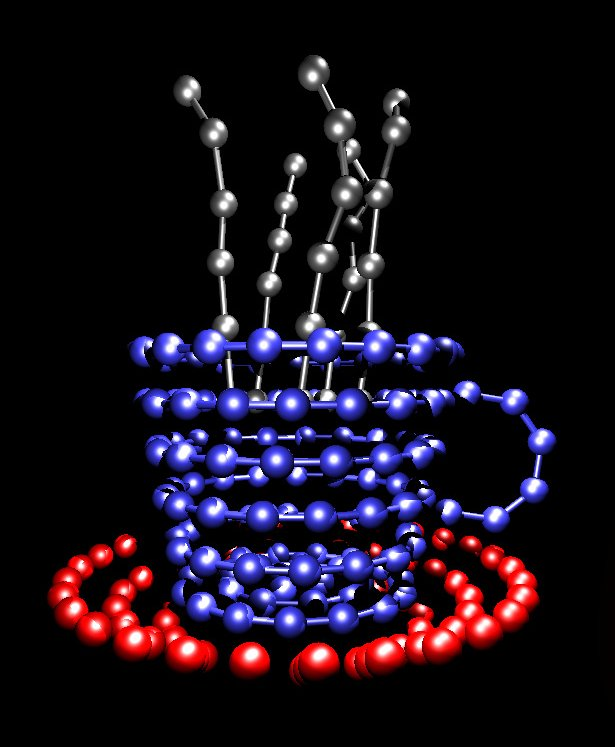
\includegraphics[width=5cm]{figures/logo}
  \end{center}
}
%\subject{}
\title{\es{} User's Guide}
%\author{}
%\date{\today}
\maketitle

\pdfbookmark{Contents}{toc}
\tableofcontents

\chapter{Introduction}
\label{chap:intro}

(new)

\begin{itemize}
\item \es{} is a generic soft matter simulation packages
\item for molecular dynamics simulations in soft matter research
\item focussed on coarse-grained models
\item employs modern algorithms (Lattice-Boltzmann, DPD, P3M, \ldots)
\item written in C for maximal portability
\item Tcl-controlled
\item parallelized
\end{itemize}

\section{Guiding principles}
\label{sec:ideas}

(from paper: 2.1 Goals and principles)

\es
\begin{itemize}
\item does \emph{not} do the physics for you!
\item requires you to understand what you do (can not be used as a
  black box)
\item gives you maximal freedom (flexibility)
\item is extensible
\item integrates system setup, simulation and analysis, as this can't
  be strictly separated in soft matter simulations
\item has no predefined units
\item sets as few defaults as possible
\end{itemize}

\section{Algorithms contained in \es}

The following algorithms are implemented in \es{}:

\begin{itemize}
\item ensembles: NVE, NVT, NpT
\item charged systems:
  \begin{itemize}
  \item P3M for fully periodic systems
  \item ELC and MMM-family of algorithms for charged systems with
    non-periodic boundary conditions
  \item Maggs algorithm 
  \end{itemize}
\item Hydrodynamics:
  \begin{itemize}
  \item DPD (as a thermostat)
  \item Lattice-Boltzmann
  \end{itemize}
\end{itemize}

\section{Basic program structure}
\label{sec:structure}

(from paper: 2.2 Basic program structure)

\begin{itemize}
\item Control level: \texttt{Tcl}
\item ``Kernel'' written in \texttt{C}
\item This user's guide will focus on the control level
\end{itemize}

\section{On units}
\label{sec:units}
\index{units}
\index{physical units}
(new)

\begin{itemize}
\item Reduced units
\item comparison to ``real units''
\item three examples on different length scales
  \begin{itemize}
  \item some atomistic model?
  \item coarse-grained model (\eg lipid bilayer)
  \item billards?
  \end{itemize}
\end{itemize}

\section{Requirements}
\label{sec:requirements}
\index{requirements}

The following libraries and tools are required to be able to compile
and use \es:

\begin{description}
\item[Tcl/Tk] \index{Tcl/Tk} \es{} requires the Toolkit Command
  Language Tcl/Tk \footnote{\url{http://www.tcl.tk/}} in the version
  8.3 or later.  Some example scripts will only work with Tcl 8.4. You
  do not only need the interpreter, but also the header files and
  libraries.  Depending on the operating system, these may come in
  separate development packages. If you want to use a graphical user
  interface (GUI) for your simulation scripts, you will also need Tk.
  
\item[FFTW] \index{FFTW} In addition, \es{} needs the FFTW library
  \footnote{\url{http://www.fftw.org/}} for Fourier transforms.
  ESPResSo can work with both the 2.1.x and 3.0.x series. Again, the
  header files are required.
  
\item[MPI] \index{MPI} Finally, if you want to use \es{} in parallel,
  you need a working MPI environment (version 1.2). Currently, the
  following MPI implementations are supported:
  \begin{itemize}
  \item LAM/MPI is the preferred variant
  \item MPICH, which seems to be considerably slower than LAM/MPI in
    our benchmarks.
  \item On AIX systems, \es{} can also use the native POE parallel
    environment.
  \item On DEC/Compaq/HP OSF/Tru64, \es{} can also use the native
    dmpirun MPI environment.
  \end{itemize}
\end{description}


\section{Syntax description}
\label{sec:syntax}

Throughout the user's guide, formal definitions of the syntax of
several Tcl- and shell-commands can be found. The following
conventions are used in these decriptions:
\begin{itemize}
\item Keywords and literals of the command that have to be typed
  exactly as given are written in \lit{typewriter} font.
\item If the command has variable arguments, they are set in
  \var{italic font}. The description following the syntax definition
  should contain a detailed explanation of the argument and its
  type.
\item \texttt{[\var{argument}]} specifies, that \var{argument} is
  optional, \ie{} it can be omitted.
\item \texttt{<\var{alt1}|\var{alt2}>} specifies, that one of the
  alternatives \var{alt1} or \var{alt2} can be used.
\end{itemize}

\minisec{Example}
\begin{code}
writevsf \var{file} [<short|verbose>] [<\var{radii}|auto>] [typedesc \var{typedesc}]
\end{code}


%%% Local Variables: 
%%% mode: latex
%%% TeX-master: "ug"
%%% End: 


\chapter{First steps}
\label{chap:firststeps}

\section{Quick installation}

\index{configure}\index{make}

If you have the requirements (see section \vref{sec:requirements})
installed, in many cases, to compile \es{}, it is enough to execute
the following sequence of two steps in the directory where you have
unpacked the sources:
\begin{code}
configure
make
\end{code}

\todo{Mention minimal configuration without myconfig.h}
In some cases, \eg{} when \es{} needs to be compiled for several
different platforms or when different versions with different sets of
features are required, it might be useful to execute the commands not
in the source directory itself, but to start \texttt{configure} from
another directory (see section \vref{sec:builddir}). Furthermore, many
features of \es{} can be selectively turned on or off in the local
configuration header of \es{} (see section \vref{sec:myconfig}) before
starting the compilation with \texttt{make}.

The shell script \texttt{configure} prepares the source code for
compilation. It will determine how to use and where to find the
different libraries and tools required by the compilation process, and
it will test what compiler flags are to be used.  The script will find
out most of these things automatically.  If something is missing, it
will complain and give hints how to solve the problem.  The
configuration process can be controlled with the help of a number of
options that are explained in section \vref{sec:configure}.

The command \texttt{make} will compile the source code. Depending on
the options passed to the program, \texttt{make} can also be used for
a number of other things:
\begin{itemize}
\item It can install and uninstall the program to some other
  directories. However, normally it is not necessary to actually
  \textit{install} \es{} to run it.
\item It can test the \es{} program for correctness.
\item It can build the documentation.
\end{itemize}
The details of the usage of \texttt{make} are described in section
\vref{sec:make}.

When these steps have successfully completed, \es{} can be started
with the command (see section \vref{sec:run})
\begin{code}
Espresso
\end{code}

\section{Running \es}

\footnote{\url{http://www.tcl.tk/man/tcl8.5/tutorial/tcltutorial.html}}

\es{} is implemented as an extension to the Tcl script language. This means that you need to write a
script for any task you want to perform with \es. To learn about the Tcl script language and
especially the \es{} extensions, this chapter offers two tutorial scripts. The first will guide you
step by step through creating your first simulation script, while the second script is a well
documented example simulation script. Since the latter is slightly more complex and uses more
advanced features of \es{}, we recommend to work through both scripts in the presented order.

\section{Creating the first simulation script}

This section introduces some of the features of \es\ by
constructing step by step a simulation script for a simple salt crystal.
We cannot give a full Tcl tutorial here; however, most of the constructs
should be self--explanatory. We also assume that the reader is familiar with the
basic concepts of a MD simulation here. The code pieces can be copied step by
step into a file, which then can be run using \verb|Espresso <file>| from the
\es source directory.

Our script starts with setting up the initial configuration.  Most conveniently,
one would like to specify the density and the number of particles of the system
as parameters:
\begin{tclcode}
set n_part 200; set density 0.7
set box_l [expr pow($n_part/$density,1./3.)]
\end{tclcode}
These variables do not change anything in the simulation engine, but are just
standard Tcl variables; they are used to increase the readability and
flexibility of the script. The box length is not a parameter of this simulation;
it is calculated from the number of particles and the system density. This
allows to change the parameters later easily, e.~g.\ to simulate a bigger
system.

The parameters of the simulation engine are modified by the \verb|setmd|
command. For example
\begin{tclcode}
setmd box_l $box_l $box_l $box_l
setmd periodic 1 1 1
\end{tclcode}
defines a cubic simulation box of size \verb|box_l|, and periodic boundary
conditions in all spatial dimensions. We now fill this simulation box with
particles
\begin{tclcode}
set q 1; set type 0
for {set i 0} { $i < $n_part } {incr i} {
  set posx [expr $box_l*[t_random]]
  set posy [expr $box_l*[t_random]]
  set posz [expr $box_l*[t_random]]
  set q [expr -$q]; set type [expr 1-$type]
  part $i pos $posx $posy $posz q $q type $type 
}
\end{tclcode}
This loop adds \verb|n_part| particles at random positions, one by one.  In this
construct, only two commands are not standard Tcl commands: the random
number generator \verb|t_random| and the \verb|part| command, which is used to
specify particle properties, here the position, the charge \verb|q| and the
type. In \es\ the particle type is just an integer number which allows to group
particles; it does not imply any physical parameters. Here we use it to tag the
charges: positive charges have type 0, negative charges have type 1.

Now we define the ensemble that we will be simulating. This is done using the
\verb|thermostat| command. We also set some integration scheme parameters:
\begin{tclcode}
setmd time_step 0.01; setmd skin 0.4
set temp 1; set gamma 1
thermostat langevin $temp $gamma
\end{tclcode}
This switches on the Langevin thermostat for the NVT ensemble, with temperature
\verb|temp| and friction \verb|gamma|. The skin depth \verb|skin| is a parameter
for the link--cell system which tunes its performance, but cannot be discussed
here.

Before we can really start the simulation, we have to specify the
interactions between our particles.  We use a simple, purely repulsive
Lennard-Jones interaction to model the hard core repulsion
\citep{grest86a}, and the charges interact via the Coulomb potential:
\begin{tclcode}
set sig 1.0; set cut   [expr 1.12246*$sig]
set eps 1.0; set shift [expr 0.25*$eps]
inter 0 0 lennard-jones $eps $sig $cut $shift 0
inter 1 0 lennard-jones $eps $sig $cut $shift 0
inter 1 1 lennard-jones $eps $sig $cut $shift 0
inter coulomb 10.0 p3m tunev2 accuracy 1e-3 mesh 32
\end{tclcode}
The first three \verb|inter| commands instruct \es\ to use the same purely
repulsive Lennard--Jones potential for the interaction between all combinations
of the two particle types 0 and 1; by using different parameters for different
combinations, one could simulate differently sized particles.  The last line sets
the Bjerrum length to the value 10, and then
instructs \es\ to use P$^3$M for the Coulombic interaction and to try to find
suitable parameters for an rms force error below $10^{-3}$, with a fixed mesh
size of 32. The mesh is fixed here to speed up the tuning; for a real
simulation, one will also tune this parameter.

If we want to calculate the temperature of our system from the kinetic energy,
we need to know the number of the degrees of freedom of the particles.
In \es\ these are usually 3 translational plus 3 rotational degrees of freedom
(if ROTATION is compiled into the code). You can get this number
in the following way \footnote{Note: there also exists a predefined tcl function {\it degrees_of_freedom} which does the same.}:

\begin{tclcode}
   if { [regexp "ROTATION" [code_info]] } { 
     set deg_free 6
   } else { set deg_free 3 }
\end{tclcode}

Now we can integrate the system:
\begin{tclcode}
set integ_steps 200
for {set i 0} { $i < 20 } { incr i} {
  set temp [expr [analyze energy kinetic]/($deg_free/2.0)*$n_part)]
  puts "t=[setmd time] E=[analyze energy total], T=$temp"
  integrate $integ_steps 
}
\end{tclcode}
This code block is the primary simulation loop and runs
$20\times$\verb|integ_steps| MD steps. Every \verb|integ_steps| time steps, the
potential, electrostatic and kinetic energies are printed out (the latter one as
temperature). However, the simulation will crash: \es\ complains about particle
coordinates being out of range. The reason for this is simple: Due to the
initial random setup, the overlap energy is around a million kT, which we first
have to remove from the system. In \es, this is can be accelerated by capping
the forces, i.~e.\ modifying the Lennard--Jones force such that it is constant
below a certain distance. Before the integration loop, we therefore insert this
equilibration loop:
\begin{tclcode}
for {set cap 20} {$cap < 200} {incr cap 20} {
  puts "t=[setmd time] E=[analyze energy total]"
  inter ljforcecap $cap; integrate $integ_steps 
}
inter ljforcecap 0
\end{tclcode}
This loop integrates the system with a force cap of initially 20 and finally
200.  The last command switches the force cap off again. With this
equilibration, the simulation script runs fine.

However, it takes some time to simulate the system, and one will probably like
to write out simulation data to configuration files, for later analysis. For
this purpose \es\ has commands to write simulation data to a Tcl stream
in an easily parsable form.  We add the following lines at end of integration
loop to write the configuration files ``config\_0'' through ``config\_19'':
\begin{tclcode}
set f [open "config_$i" "w"]
blockfile $f write tclvariable {box_l density}
blockfile $f write variable box_l
blockfile $f write particles {id pos type}
close $f
\end{tclcode}
The created files ``config\_...'' are human--readable and look like
\begin{tclcode}
{tclvariable
        {box_l 10}
        {density 0.7}
}
{variable  {box_l 10.0 10.0 10.0} }
{particles {id pos type}
        {0 3.51770181433 4.3208975936 5.30529948918 0}
        {1 3.93145531704 6.58506447035 6.95045147034 1}
        ...
}
\end{tclcode}
As you can see, such a \emph{blockfile} consists of several Tcl lists,
which are called \emph{blocks}, and can store any data available from the
simulation. Reading a configuration is done by the following simple script:
\begin{tclcode}
set f [open $filename "r"]
while { [blockfile $f read auto] != "eof" } {}
close $f
\end{tclcode}
The \verb|blockfile read auto| commands will set the Tcl variables \verb|box_l|
and \verb|density| to the values specified in the file when encountering the
\verb|tclvariable| block, and set the box dimensions for the simulation when
encountering the \verb|variable| block. The particle positions and types of all
216 particles are restored when the \verb|particles| block is read. Note that it
is important to have the box dimensions set before reading the particles, to
avoid problems with the periodic boundary conditions.

\begin{figure}[tb]
  \centering
  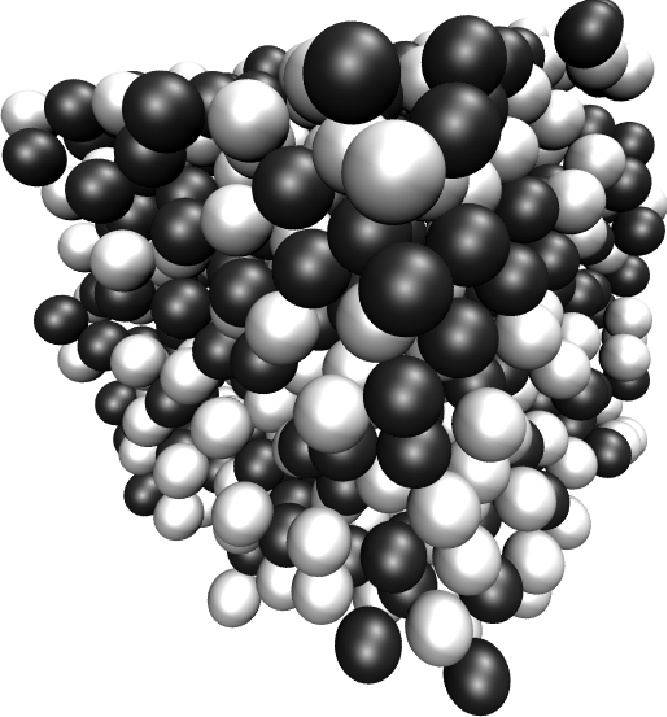
\includegraphics[width=0.4\textwidth]{figures/salt.png}
  \caption{VMD Snapshot of the salt system}
  \label{fig:snapshot}
\end{figure}

With these configurations, we can now investigate the system. As an example, we
will create a second script which calculates the averaged radial distribution
functions $g_{++}(r)$ and $g_{+-}(r)$. The radial distribution function for a
the current configuration can be obtained using the \verb|analyze| command:
\begin{tclcode}
set rdf [analyze rdf 0 1 0.9 [expr $box_l/2] 100]
set rlist ""
set rdflist ""
foreach value [lindex $rdf 1] {
  lappend rlist   [lindex $value 0]
  lappend rdflist [lindex $value 1] 
}
\end{tclcode}
The shown \verb|analyze rdf| command returns the distribution function of
particles of type 1 around particles of type 0 (i.~e.\ of opposite charges) for
radii between $0.9$ and half the box length, subdivided into $100$ bins.
Changing the first two parameters to either ``0 0'' or ``1 1'' allows to
determine the distribution for equal charges. The result is a list of $r$ and
$g(r)$ pairs, which the following foreach loop divides up onto two lists
\verb|rlist| and \verb|rdflist|.

To average over a set of configurations, we put the two last code snippets into
a loop like this:
\begin{tclcode}
set cnt 0
for {set i 0} {$i < 100} {incr i} { lappend avg_rdf 0}
foreach filename $argv {
  set f [open $filename "r"]
  while { [blockfile $f read auto] != "eof" } {}
  close $f
  set rdf [analyze rdf 0 1 0.9 [expr $box_l/2] 100]
  set rlist ""
  set rdflist ""
  foreach value [lindex $rdf 1] {
     lappend rlist   [lindex $value 0]
     lappend rdflist [lindex $value 1] }
  set avg_rdf [vecadd $avg_rdf $rdflist]
  incr cnt 
}
set avg_rdf [vecscale [expr 1.0/$cnt] $avg_rdf]
\end{tclcode}
Initially, the sum of all $g(r)$, which is stored in \verb|avg_rdf|, is set to
0.  Then the loops over all configurations given by \verb|argv|, calculates
$g(r)$ for each configuration and adds up all the $g(r)$ in \verb|avg_rdf|.
Finally, this sum is normalized by dividing by the number of
configurations. Note the ``1.0/\$cnt''; this is necessary, since ``1/\$cnt'' is
interpreted as an integer division, which results in 0 for $\text{cnt}>1$.
\verb|argv| is a predefined variable: it contains all the command line
parameters. Therefore this script should be called like
\begin{code}
Espresso \var{script} [\var{config}... ]
\end{code}

\begin{figure}[tb]
  \centering
  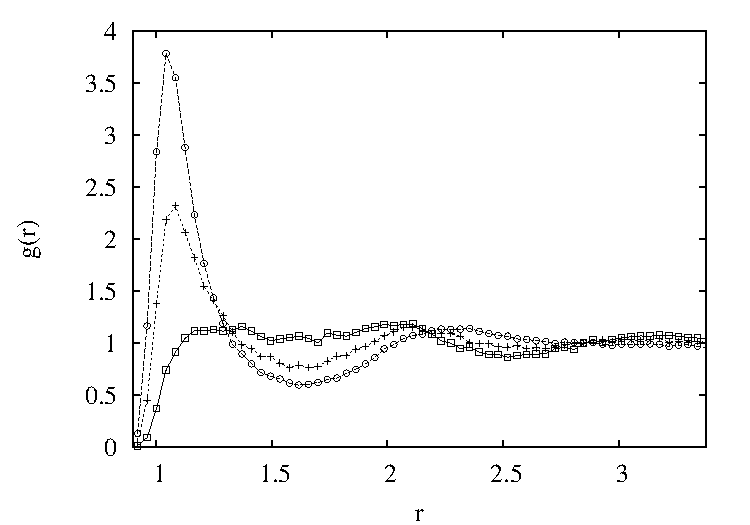
\includegraphics[width=0.7\textwidth]{figures/nacl-rdf.pdf}
  \caption{Radial distribution functions $g_{++}(r)$ between equal charges
    (rectangles) and $g_{+-}(r)$ for opposite charges (circles). The plus
    symbols denote $g(r)$ for an uncharged system.}
  \label{fig:rdf}
\end{figure}

The printing of the calculated radial distribution functions is simple. Add to the end of the
previous snippet the following lines:
\begin{tclcode}
set plot [open "rdf.data" "w"]
puts $plot "\# r rdf(r)"
foreach r $rlist rdf $avg_rdf { puts $plot "$r $rdf" }
close $plot
\end{tclcode}
This instructs the Tcl interpreter to write the \verb|avg_rdf| to the file \verb|rdf.data| in
gnuplot--compatible format. Fig.~\ref{fig:rdf} shows the resulting radial distribution functions,
averaged over 100 configurations. In addition, the distribution for a neutral
system is given, which can be obtained from our simulation script by simply
removing the command \verb|inter coulomb ...| and therefore not turning on P$^3$M.

The code example given before is still quite simple, and the reader is
encouraged to try to extend the example a little bit, e.~g. by using differently
sized particle, or changing the interactions. If something does not work, \es\
will give comprehensive error messages, which should make it easy to identify
mistakes. For real simulations, the simulation scripts can extend over thousands
of lines of code and contain automated adaption of parameters or online
analysis, up to automatic generation of data plots.  Parameters can be changed
arbitrarily during the simulation process, as needed for e.~g.\ simulated
annealing. The possibility to perform non--standard simulations without the need
of modifications to the simulation core was one of the main reasons why we
decided to use a script language for controlling the simulation core.

\section{\texttt{tutorial.tcl}}

In the directory \texttt{samples/} of the es{} sources, you will find
a well documented simulation script \texttt{tutorial.tcl}, which takes
you step by step through a slightly more complicated simulation of a
polyelectrolyte system. The basic structure of the script is however
the same as in the previous example and probably the same as the
structure of most \es{} simulation scripts.

Initially, some parameters and global variables are set, the
interactions are initialized, and particles are added. For this, the
script makes use of the \verb|polymer| command, which provides a
faster way to set up chain molecules.

The actual simulation falls apart again into two loops, the warmup
loop with increasing force capping, and the final simulation loop.
Note that the electrostatic interaction is only activated after
equilibrating the excluded volume interactions, which speeds up the
warmup phase. However, depending on the problem, this splitted warmup
may not be possible due to physical restrictions. \es{} cannot detect
these mistakes and it is your responsibility to find simulation
procedure suitable to your specific problem.

%%% Local Variables: 
%%% mode: latex
%%% TeX-master: "ug"
%%% End: 

\chapter{Installation}
\label{chap:install}
\index{Installation|textbf}

\begin{itemize}
\item Compiling \es{} is a necessary evil
\item Features can be compiled in or not
\item For maximal efficiency, compile in only the features that you
  use
\item \es{} can be obtained from the \es{} home page
  \footnote{\url{http://www.espresso.mpg.de}}.
\end{itemize}



\section{Requirements}
\label{sec:requirements}
\index{requirements}

\begin{description}
\item[Tcl/Tk] \index{Tcl/Tk} \es{} requires the Toolkit Command
  Language Tcl/Tk \footnote{\url{http://www.tcl.tk/}} in the version
  8.3 or later.  Some example scripts will only work with Tcl 8.4. You
  do not only need the interpreter, but also the header files and
  libraries.  Depending on the operating system, these may come in
  separate development packages. If you want to use a graphical user
  interface (GUI) for your simulation scripts, you will also need Tk.
  
\item[FFTW] \index{FFTW} In addition, \es{} needs the FFTW library
  \footnote{\url{http://www.fftw.org/}} for Fourier transforms.
  ESPResSo can work with both the 2.1.x and 3.0.x series. Again, the
  header files are required.
  
\item[MPI] \index{MPI} Finally, if you want to use ESPResSo in
  parallel, you need a working MPI environment (version 1.2). ESPResSo
  currently supports the following MPI implementations:
  \begin{itemize}
  \item LAM/MPI is the preferred variant
  \item MPICH, which seems to be considerably slower than LAM/MPI in
    our benchmarks.
  \item On AIX systems, \es{} can also use the native POE parallel
    environment.
  \item On DEC/Compaq/HP OSF/Tru64, \es{} can also use the native
    dmpirun MPI environment.
  \end{itemize}
\end{description}

\section{Quick start}

\index{configure}\index{make}

In many cases, to compile \es{}, it is enough to execute the following
sequence of two steps in the directory where you have unpacked the
sources:
\begin{verbatim}
> configure
> make
\end{verbatim}

In some cases, \eg{} when \es{} needs to be compiled for several
different platforms or when different versions with different sets of
features are required, it might be useful to execute the commands not
in the source directory itself, but to start \texttt{configure} from
another directory (see section \vref{sec:builddir}). Furthermore, many
features of \es{} can be selectively turned on or off in the local
configuration header of \es{} (see section \vref{sec:myconfig}) before
starting the compilation with \texttt{make}.

The shell script \texttt{configure} prepares the source code for
compilation. It will determine how to use and where to find the
different libraries and tools required by the compilation process, and
it will test what compiler flags are to be used.  The script will find
out most of these things automatically.  If something is missing, it
will complain and give hints how to solve the problem.  The
configuration process can be controlled with the help of a number of
options that are explained in section \vref{sec:configure}.

The command \texttt{make} will compile the source code. Depending on
the options passed to the program, \texttt{make} can also be used for
a number of other things:
\begin{itemize}
\item It can install and uninstall the program to some other
  directories. However, normally it is not necessary to actually
  \textit{install} \es{} to run it.
\item It can test the \es{} program for correctness.
\item It can build the documentation.
\end{itemize}
The details of the usage of \texttt{make} are described in section
\vref{sec:make}.

When these steps have successfully completed, \es{} can be started
with the command (see section \vref{sec:run})
\begin{verbatim}
> Espresso
\end{verbatim}

\section{Source and build directory}
\label{sec:builddir}
\index{build directory} \index{source directory}

If you plan to use \es{} with a single configuration, you can skip the
rest of this section. If then you have problems finding the \es{}
binary or you come upon a reference to the \emph{build directory} in
the documentation, you might have to read it, anyway. In this case,
you might also want to focus on section
\vref{sec:compiling_in_srcdir}.

Usually, when a program is compiled, the resulting binary files are
put into the same directory as the sources of the program. In \es{},
the \emph{source directory} that contains all the source files can be
completely separated from the \emph{build directory} where the files
created by the build process are put. As the source directory is not
touched during the compilation process, it is possible to compile more
than one binary version of \es{} from the same set of source files.
This is useful in cases when \es{} is to be used on different computer
hardware or with a different configuration.

The source directory is the directory that contains the source files.
The location of the build directory is determined when the
\texttt{configure}-script is called.  Usually, the build directory is
assigned to the current working directory when the
\texttt{configure}-script was called. All further commands concerning
compiling and running \es{} have to be called from this directory.

\paragraph{Example}
When the source directory is \texttt{\$srcdir} (\ie{} the files where
unpacked to this directory), then the build directory can be set to
\texttt{\$builddir} by calling the \texttt{configure}-script from
there:
\begin{verbatim}
> cd $builddir
> $srcdir/configure
> make
> Espresso
\end{verbatim}

\subsection{Compiling in the source directory}
\label{sec:compiling_in_srcdir}

It is possible to run the commands \texttt{configure}, \texttt{make}
and \texttt{Espresso} directly in the source directory. In this case,
the \es{} build system is also prepared to handle different platforms.

When \texttt{configure} is from the source directory, a new
subdirectory is created and \texttt{configure} is recursively called
from this directory, making the subdirectory the build directory.  The
directory is called \texttt{obj-}\textit{platform}\texttt{/}, where
\textit{platform} is a descriptor of the CPU type where the script was
started, \eg{} \texttt{obj-Athlon\_64-pc-linux}.

Furthermore, the option \texttt{--enable-chooser} will be set in the
recursive call of \texttt{configure}, that influences how the
installed \es{} binary is found.

\section{The configuration header \texttt{myconfig.h}}
\label{sec:myconfig}

\index{myconfig.h} \index{configuration header} \es{} has a great
number of features that can be compiled into the binary (see chapter
\vref{chap:features}).  However, it is not recommended to actually
compile in all possible features, as this will negatively affect \es's
performance. Instead, compile in only the features that are actually
required. For the developers, it is also possible to turn on or off a
number of debugging messages. The features and debug messages can be
controlled via a configuration header file that contains
C-preprocessor declarations.

By default, the configuration header is called \texttt{myconfig.h}.
The name of the configuration header can be either changed when the
\texttt{configure}-script is called with the option
\texttt{--with-myconfig} (see section \vref{sec:configure}), or when
\texttt{make} is called with the setting
\texttt{myconfig=}\textit{myconfig\_header} (see section
\vref{sec:make}).

The configuration header can be put in the build directory, or in the
source directory. When a configuration header is found in both
directories, the one in the build directory will be used. If both
directories do not contain a configuration header, a default header
will be used that turns on the default features.

The file \texttt{myconfig-sample.h} in the source directory contains
an example configuration header.

\paragraph{Example}
The configuration header can be used to compile different versions
from the same source directory. Suppose that you have a source
directory \texttt{\$srcdir} and two build directories
\texttt{\$builddir1} and \texttt{\$builddir2} that contain different
configuration headers:

\begin{itemize}
\item \texttt{\$builddir1/myconfig.h}:
\begin{verbatim}
#define ELECTROSTATICS
#define LENNARD-JONES
\end{verbatim}

\item \texttt{\$builddir2/myconfig.h}:
\begin{verbatim}
#define LJCOS
\end{verbatim}
\end{itemize}

\noindent Then you can simply compile two different versions of \es{} via
\begin{verbatim}
cd $builddir1
$srcdir/configure
make

cd $builddir2
$srcdir/configure
make
\end{verbatim}

\section{Running configure}
\label{sec:configure}

\texttt{configure} will save the assembled information in the
different \texttt{Makefile}s, the header file \texttt{acconfig.h}, and
some other shell scripts required later on.

The following options are recognised by \texttt{configure}:
\begin{verbatim}
--prefix=PREFIX (Default: $HOME/Espresso)
--exec-prefix=EXEC_PREFIX (DEFAULT: PREFIX)

--enable-chooser (Default: depends on current directory)
--with-myconfig=MYCONFIG_HEADER (Default: myconfig.h)
--enable-config=KNOWN_CONFIG (Default: no)
--enable-debug (Default: off)
--enable-profiling (Default: off)
--disable-processor-optimization (Default: enabled)
--enable-xlc-qipa (Default: yes)

--with-mpi=MPI (Default: guess)
--with-efence (Default: no)
--with-tcl=VERSION (Default: guess)
--with-tk[=VERSION] (Default: no)
--with-fftw=VERSION (Default: guess)
\end{verbatim}

The following variables have an influence on the compilation:

\begin{verbatim}
CC	gives the compiler to use. Note that MPI environments often need special
	compilers rsp. wrapper scripts.
CFLAGS	flags used in the object file compilation pass. Typically you will specify
	additional include paths here, e.g. "-I/home/me/include", but also other
	compiler flags such as "-O5" are possible. In the latter case, you will
	probably want to disable the automated CPU optimization detection via
	"--disable-processor-optimization".
LDFLAGS the same as CFLAGS for the linking pass. Note that you should NOT
	specify libraries here, since for some compilers they have to appear at
	the end of the line, only additional library paths, e.g. "-L/home/me/lib".
LIBS	Use this variable to specify additional libraries to link against, e.g.
	"-lmycoollib".
\end{verbatim}

\section{Compiling, testing and installing \es}
\label{sec:make}

\begin{verbatim}
> make [all] [myconfig=MYCONFIG_HEADER]

  Compiles Espresso. 

  Variables:
  ----------
  myconfig=MYCONFIG_HEADER
    Sets the name of the local configuration header file where you can
    turn on the different features and debug messages.
    This can be useful if you want to compile Espresso with different
    sets of features from the same sources.
    WARNING:
    If you use this when compiling Espresso, it is necessary to use
    the same setting when you recompile Espresso or to call "make
    clean" before. Otherwise, you will end up with an inconsistent
    version of Espresso.
    DO NOT USE THIS WHEN YOU WORK ON THE SOURCE CODE! 
    USE configure --with-myconfig instead!

> make check [processors=PROC] [tests=TESTS]

  Runs the Espresso testsuite.

  Variables:
  ----------
  processors=PROC (Default: "1 2 3 4 6 8")
    Sets the list of processor numbers that are to be tested,
    e.g. 'make check processors="1 2"' will run the testsuite on only
    one and two processors. 

  tests=TESTS (Default: all tests)
    Sets the tests of the testsuite that are run, e.g. 
    'make check tests="madelung.tcl"' will run only the test
    madelung.tcl.

> make clean

  Deletes the files that were created during the compilation.

> make mostlyclean

  Deletes most files that were created during the compilation. Will
  keep for example the built doxygen documentation and the Espresso
  binary.

> make dist [internal=1]

  Creates a .tar.gz-file of the Espresso sources. This will include all
  source files of Espresso as they currently are in the source
  directory, i.e. it will include local changes.
  This is useful to give your version of Espresso to other people.

  Variables:
  ----------
  internal=1
    When this is give, include the "internal" directory into the
    distribution file.

> make dist-internal

  Same as "make dist internal=1"

> make install [prefix=DIR] [exec-prefix=DIR]

  Installs Espresso.

  Variables:
  ----------
  prefix=PREFIX (Default: configure option --prefix)
    Sets the directory where to install Espresso. This
    defaults to the directory given to configure.

  exec-prefix=PREFIX (Default: configure option --exec-prefix)
    Sets the directory where to install the executable files of
    Espresso. This is only required, when the executable files are to
    be installed into some architecture-specific directory. Otherwise,
    it is identical to the prefix.

> make uninstall [prefix=DIR] [exec-prefix=DIR]

  Uninstalls Espresso. The variables are identical to the variables of
  "make install".
\end{verbatim}

\section{Running \es}
\label{sec:run}

A number of wrapper scripts are used in running \es{}:
\begin{itemize}
\item The script \texttt{Espresso} in the source and build directory
  will try to run the compiled version of \es. If it is called from
  the source directory, it assumes that \es{} was also configured in
  the source directory and will try to recursively start the script in
  the corresponding \texttt{obj-PLATFORM} build directory. If it is
  called in the build directory, it will start the \es-binary with the
  right MPI implementation.
\item The chooser script \texttt{Espresso} 
  \begin{itemize}
  \item installed when \verb!--enable-chooser! was given
  \item installed to bindir
  \item tries to run the correct version of the MPI-wrapper
    \texttt{Espresso}
  \end{itemize}
\item The MPI-wrapper \texttt{Espresso}
  \begin{itemize}
  \item installed next to \es{} binary
  \item starts the binary with the right MPI implementation
  \end{itemize}
\item The \es{} binary \texttt{Espresso-bin} can also be started
  directly, however, it requires that the environment variable
  \verb!ESPRESSO_SCRIPTS! is set to the directory where the scripts
  are installed (usually \verb!$(prefix)/lib/espresso/scripts! or
  \verb!$(prefix)/share/espresso/scripts!).
\end{itemize}

\es{} can be run via
\begin{syntax}
$>$ Espresso \var{tcl\_script} \var{N\_processors} \var{args}
\end{syntax}

Note that depending on your MPI installation, MPI jobs can only be run
in the queueing system, so that ESPResSo will not run from the command
line. In that case, you may not be able to run the testsuite, or have
to directly submit the testsuite script \verb!testsuite/test.sh! to
the queueing system.


%%% Local Variables: 
%%% mode: latex
%%% TeX-master: "ug"
%%% End: 


\chapter{Setting up particles}
\label{chap:part}

\section{\texttt{part}: Creating single particles}
\newescommand{part}

\subsection{Defining particle properties}

\begin{essyntax}
  part
  \var{particle_number}
  \opt{pos \var{x} \var{y} \var{z}}
  \opt{type \var{particle_type_number}}
  \opt{v \var{vx} \var{vy} \var{vz}}
  \opt{f \var{fx} \var{fy} \var{fz}}
  \opt{bond \var{bond_type_number} \var{partner} \dots}
  \require{1}{\opt{q \var{charge}}}
  \require{2}{\opt{quat \var{q1} \var{q2} \var{q3} \var{q4}}}
  \require{2}{\opt{omega \var{x_value} \var{y_value} \var{z_value}}}
  \require{2}{\opt{torque \var{x_value} \var{y_value} \var{z_value}}}\\
  \require{3}{\opt{\opt{un}fix \var{x} \var{y} \var{z}}}
  \require{3}{\opt{ext_force \var{x_value} \var{y_value} \var{z_value}}}
  \require{4}{\opt{exclude \var{exclusion_partner}\dots}}
  \require{4}{\opt{exclude delete \var{exclusion_partner}\dots}}
  \require{5}{\opt{mass \var{mass}}}
  \require{6}{\opt{dipm \var{moment}}}
  \require{6}{\opt{dip \var{dx} \var{dy} \var{dz}}}
  \begin{features}
    \required[1]{ELECTROSTATICS} 
    \required[2]{ROTATION}
    \required[3]{EXTERNAL_FORCES}
    \required[4]{EXCLUSION}
    \required[5]{MASS}
    \required[6]{DIPOLES}
  \end{features}
\end{essyntax}

This command modifies particle data, namely position, type (monomer,
ion, \dots), charge, velocity, force and bonds. Multiple properties can
be changed at once. If you add a new particle the position has to be
set first because of the spatial decomposition.

\begin{arguments}
\item[\var{particle_number}]
\item[\opt{pos \var{x} \var{y} \var{z}}] Sets the position of this
  particle to $(x,y,z)$.
\item[\opt{type \var{particle_type_number}}] Restrictions:
  $\var{particle_type_number} \geq 0$.\\ The
  \var{particle_type_number} is used in the \keyword{inter} command
  (see section \vref{tcl:inter}) to define the parameters of the non
  bonded interactions between different kinds of particles.
\item[\opt{v \var{vx} \var{vy} \var{vz}}] Sets the velocity of
this particle to $(vx,vy,vz)$. The velocity remains variable and will be changed
during integration.
\item[\opt{f \var{fx} \var{fy} \var{fz}}] Set the force acting on this particle
to $(fx,fy,fz)$. The force remains variable and will be changed during integration.
\item[\opt{bond \var{bond_type_number} \var{partner}+}]
  Restrictions: \var{bond_type_number} $\geq 0$; \var{partner} must
  be an existing particle.  The \var{bond_type_number} is used for
  the inter command to define bonded interactions.
\item[bond delete] Will delete all bonds attached to this particle.
\item[\opt{q \var{charge}}] Sets the charge of this praticle to $q$.
\item[\opt{quat \var{q1} \var{q2} \var{q3} \var{q4}}] \todo{Docs required (JC?).} 
  \item[\opt{omega \var{x_value} \var{y_value} \var{z_value}}] \todo{Docs
  required (JC?).} 
  \item[\opt{torque \var{x_value} \var{y_value} \var{z_value}}] \todo{Docs
  required (JC?).}
\item[\opt{fix \var{x} \var{y} \var{z}}] Fixes the particle in space.
  By supplying a set of 3 integers as arguments it is possible to fix
  motion in \var{x}, \var{y}, or \var{z} coordinates independently. For
  example \var{fix 0 0 1} will fix motion only in z. Note that
  \var{fix} without arguments is equivalent to \var{fix 1 1 1}.
\item[\opt{ext_force \var{x_value} \var{y_value} \var{z_value}}]
  An additional external force is applied to the particle.
\item[\opt{unfix}] Release any external influence from the particle.
\item[\opt{exclude \var{exclusion_partner}+}] Restrictions:
  \var{exclusion_partner} must be an existing particle.  Between the
  current particle an the exclusion partner(s), no nonbonded
  interactions are calculated. Note that unlike bonds, exclusions are
  stored with both partners.  Therefore this command adds the defined
  exclusions to both partners.
\item[\opt{exclude delete \var{exclusion_partner}+}] Searches for the
  given exclusion and deletes it. Again deletes the exclusion with
  both partners.
  \item[\opt{mass \var{mass}}] Sets the mass of this particle to $mass$. If not
  set, all particles have a mass of 1 in reduced units.
  \item[\opt{dipm \var{moment}}] Sets the dipol moment of this particle to $moment$.
  \item[\opt{dip \var{dx} \var{dy} \var{dz}}] Sets the orientation of the
  dipol axis to $(dx,dy,dz)$.
 
  \end{arguments}
\subsection{Getting particle properties}

\begin{essyntax}
  \variant{1}
  part \var{particle_number} print
  \optlong{\alt{id \asep pos \asep type \asep folded_position \asep type \asep
      q \asep v \asep f \asep fix \asep ext_force \asep bond \asep
      \mbox{connections \opt{\var{range}}}}}\dots
  \variant{2} part
\end{essyntax}

Variant \variant{1} will return a list of the specified properties of
particle \var{particle_number}, or all properties, if no keyword is
specified.  Variant \variant{2} will return a list of all properties
of all particles.

\minisec{Example}
\begin{code}
part 40 print id pos q bonds
\end{code}
will return a list like
\begin{tclcode}
40 8.849 1.8172 1.4677 1.0 {}
\end{tclcode}
This routine is primarily intended for effective use in Tcl scripts.

When the keyword \keyword{connection} is specified, it returns the
connectivity of the particle up to \var{range} (defaults to 1). For
particle 5 in a linear chain the result up to \var{range} = 3 would
look like:
\begin{tclcode}
{ { 4 } { 6 } } { { 4 3 } { 6 7 } } { {4 3 2 } { 6 7 8 } } 
\end{tclcode}
The function is useful when you want to create bonded interactions to
all other particles a certain particle is connected to. Note that this
output can not be used as input to the part command. Check results if
you use them in ring structures.

If none of the options is specified, it returns all properties of the
particle, if it exists, in the form
\begin{tclcode}
  0 pos 2.1 6.4 3.1 type 0 q -1.0 v 0.0 0.0 0.0 f 0.0 0.0 0.0
  bonds { {0 480} {0 368} ... } 
\end{tclcode}
which may be used as an input to this function later on. The first
integer is the particle number.

Variant \variant{2} returns the properties of all stored particles in
a tcl-list with the same format as specified above:
\begin{tclcode}
{0 pos 2.1 6.4 3.1 type 0 q -1.0 v 0.0 0.0 0.0 f 0.0 0.0 0.0
 bonds{{0 480}{0 368}...}} 
{1 pos 1.0 2.0 3.0 type 0 q 1.0 v 0.0 0.0 0.0 f 0.0 0.0 0.0
 bonds{{0 340}{0 83}...}} 
{2...{{...}...}}
{3...{{...}...}}
...
\end{tclcode}

\subsection{Deleting  particles}
\label{tcl:part:delete}

\begin{essyntax}
  \variant{1} part \var{particle_number} delete
  \variant{2} part deleteall
\end{essyntax}

In variant \variant{1}, the particle \var{particle_number} is deleted
and all bonds referencing it.  Variant \variant{2} will delete all
particles currently present in the simulation. Variant \variant{3}
will delete all currently defined exclusions.

\subsection{Exclusions}

\begin{essyntax}
  \variant{1} part auto_exclusions \opt{\var{range}}
  \variant{2} part delete_exclusions
\end{essyntax}

Variant \variant{1} will create exclusions for all particles pairs
connected by not more than \var{range} bonds (\var{range} defaults to
2). This is typically used in atomistic simulations, where nearest and
next nearest neighbour interactions along the chain have to be omitted
since they are included in the bonding potentials. For example, if the
system contains particles $0$ \dots $100$, where particle $n$ is
bonded to particle $n-1$ for $1 \leq n \leq 100$, then it will result
in the exclusions:
\begin{itemize}
  \item particle 1 does not interact with particles 2 and 3
  \item particle 2 does not interact with particles 1, 3 and 4
  \item particle 3 does not interact with particles 1, 2, 4 and 5
  \item ...
\end{itemize}

Variant \variant{2} deletes all exclusions currently present in the
system.

\section{Creating groups of particle}

\subsection{\texttt{polymer}: Setting up polymer chains}

\newescommand{polymer}
\begin{essyntax}
  polymer 
  \var{num_polymers} \var{monomers_per_chain}
  \var{bond_length}\\
  \opt{start \var{part_id}} 
  \opt{pos \var{x} \var{y} \var{z}}
  \opt{mode \alt{RW \asep SAW \asep PSAW} 
    \opt{\var{shield} \opt{\var{max_try}}}} 
  \require{1}{\opt{charge \var{val_charged_monomer}}} 
  \require{1}{\opt{distance \var{dist_charged_monomer}}}
  \opt{types \var{type_neutral_monomer}
    \opt{\var{type_charged_monomer}}} 
  \opt{bond \var{type_bond}} 
  \opt{angle \var{phi} \opt{\var{theta} \opt{\var{x} \var{y}
        \var{z}}}}
  \require{2}{\opt{constraints}}
  \begin{features}
    \required[1]{ELECTROSTATICS}
    \required[2]{CONSTRAINTS}
  \end{features}
\end{essyntax}

This command will create \var{num_polymers} polymer or
polyelectrolyte chains with \var{monomers_per_chain} monomers per
chain. The length of the bond between two adjacent monomers will be
set up to be \var{bond_length}.

\begin{arguments}
\item[\var{num_polymers}] Sets the number of polymer chains.
\item[\var{monomers_per_chain}] Sets the number of monomers per
  chain.
\item[\var{bond_length}] Sets the initial distance between two adjacent
  monomers. The distance during the course of the simulation depends on the
  applied potentials. For fixed box length please refer to the SHAKE algorithm.
  \todo{Link to rattle/shake.}
\item[\opt{start \var{part_id}}] Sets the particle number of the
  start monomer to be used with the \keyword{part} command. This
  defaults to 0.

\item[\opt{pos \var{x} \var{y} \var{z}}] Sets the position of the
  first monomer in the chain to \var{x}, \var{y}, \var{z} (defaults to
  a randomly chosen value)
  
\item[\opt{mode \alt{RW  \asep  PSAW  \asep  SAW} \opt{\var{shield}
      \opt{\var{max_try}}}}]
  Selects the setup mode:
  \begin{description}
  \item[\keyword{RW} (Random walk)] The monomers are
    randomly placed by a random walk with a steps size of
    \var{bond_length}.
  \item[\keyword{PSAW} (Pruned self-avoiding walk)] The position of a
    monomer is randomly chosen in a distance of \var{bond_length} to
    the previous monomer. If the position is closer to another
    particle than \var{shield}, the attempt is repeated up to
    \var{try_max} times. Note, that this is not a real self-avoiding
    random walk, as the particle distribution is not the same. If you
    want a real self-avoiding walk, use the \keyword{SAW} mode.
    However, \keyword{PSAW} is several orders of magnitude faster than
    \keyword{SAW}, especially for long chains.
  \item[\keyword{SAW} (Self-avoiding random walk)] The positions of
    the monomers are chosen as in the plain random walk. However, if
    this results in a chain that has a monomer that is closer to
    another particle than \var{shield}, a new attempt of setting up
    the whole chain is done, up to \var{max_try} times.
  \end{description}
  The default for the mode is \keyword{RW}, the default for the
  \var{shield} is $1.0$, and the default for \var{max_try} is
  $30000$, which is usually enough for \keyword{PSAW}. Depending on
  the length of the chain, for the \keyword{SAW} mode, \var{max_try}
  has to be increased by several orders of magnitude.
\item[\opt{charge \var{val_charged_monomer}}] Sets the valency of
  the charged monomers.  If the valency of the charged polymers
  \var{val_charged_monomer} is smaller than $10^{-10}$, the charge
  is assumed to be zero, and the types are set to
  \var{type_charged_monomer} = \var{type_neutral_monomer}. If charge is not set,
  it defaults to 0.0.

\item[\opt{distance \var{dist_charged_monomer}}] Sets the stride
  between the indices of two charged monomers. This defaults defaults
  to 1, meaning that all monomers in the chain are charged.
  
\item[\opt{types \var{type_neutral_monomer}
    \var{type_charged_monomer}}] Sets the type numbers of the
  neutral and charged monomer types to be used with the \keyword{part}
  command. If \var{type_neutral_monomer} is defined,
  \var{type_charged_monomer} defaults to 1. If the option is
  omitted, both monomer types default to 0.
  
\item[\opt{bond \var{type_bond}}] Sets the type number of the bonded
  interaction to be set between the monomers. This defaults to 0. Any bonded
  interaction, no matter how many bonding-partners needed, is stored with the
  second particle in this bond. \todo{Link to
  bonded interactions}
  
\item[\opt{angle \var{phi} [\var{theta} [\var{x} \var{y} \var{z}]]}]
  Allows for setting up helices or planar polymers: \var{phi} sets
  the angle $\phi$ and \var{theta} sets the angle $\theta$ between
  adjacent bonds. \var{x}, \var{y} and \var{z} set the position of the
  second monomer of the first chain.
  \item[\opt{constraints}] If this option is specified, the particle setup-up
  tries to obey previously defined constraints (see Section \vref{sec:constraint}).
\end{arguments}

\subsection{\texttt{counterions}: Set up counterions}
\newescommand{counterions}
\begin{essyntax}
  counterions
  \var{N_CI} 
  \opt{start \var{part_id}} 
  \opt{mode \alt{SAW \asep RW} \opt{\var{shield} \opt{\var{max_try} }}} 
  \require{1}{\opt{charge \var{val_CI}}}
  \opt{type \var{type_CI}}
  \begin{features}
    \required[1]{ELECTROSTATICS}
  \end{features}
\end{essyntax}
This command will create \var{N_CI} counterions in the simulation box.
\begin{arguments}
  \item[\var{N_CI}] Sets the number of counterions to setup.
  \item[\opt{start \var{part_id}}] Sets the particle id of the first counterion.
  It defaults to the current number of particles, \ie counterions are placed
  after all previously defined particles.
  \item[\opt{mode \alt{SAW \asep RW} \opt{\var{shield} \opt{\var{max_try} }}}]
  Specifies the setup method to place the counterions. It defaults to
  \texttt{SAW}. See the \texttt{polymer} command for a detailed description.
  \item[\opt{charge \var{val_CI}}] Specifies the charge of the counterions. If not
  set, it defaults to -1.0.
  \item[\opt{type \var{type_CI}}] Specifies the particle type of the counterions. It
  defaults to 2.
\end{arguments}

\smallskip
\subsection{\texttt{salt}: Set up salt ions}
\newescommand{salt}
\begin{essyntax}
  salt 
  \var{N_pS} \var{N_nS} 
  \opt{start \var{part_id}} 
  \opt{mode \alt{SAW \asep RW} \opt{\var{shield} \opt{\var{max_try}}}}
  \require{1}{\opt{charges \var{val_pS} \opt{\var{val_nS}}}} 
  \opt{types \var{type_pS} \opt{\var{type_nS}}}
  \opt{rad \var{radius}}
  \begin{features}
    \required[1]{ELECTROSTATICS}
  \end{features}
\end{essyntax}

Create \var{N_pS} positively and \var{N_nS} negatively charged salt
ions of charge \var{val_pS} and \var{val_nS} within the simulation
box.
\begin{arguments}
  \item[\var{N_pS}] Sets the number of positively charged salt ions.
  \item[\var{N_nS}] Sets the number of negatively charged salt ions.
  \item[\opt{start \var{part_id}}] Sets the particle id of the first
  (positively charged) salt ion. It defaults to the current number of particles.
  \item[\opt{mode \alt{SAW \asep RW} \opt{\var{shield} \opt{\var{max_try} }}}]
  Specifies the setup method to place the counterions. It defaults to 
  \texttt{SAW}. See the \texttt{polymer} command for a detailed description.
  \item[\opt{charge \var{val_pS} \opt{\var{val_nS}}}] Sets the charge of the
  positive salt ions to \var{val_pS} and the one of the negatively charged salt
  ions to \var{val_nS}. If not set, the values default to 1.0 and -1.0.
  \item[\opt{type \var{type_pS} \opt{\var{type_nS}}}] Specifies the particle type of the
  salt ions. It defaults to 3 for positive ions and 4 for negative ions.
  \item[\opt{rad \var{radius}}] When working within the cell model, the salt
  ions are only placed in a sphere with radius \var{radius} around the origin. 
\end{arguments}


\subsection{\texttt{diamond}: Setting up diamond polymer networks}
\newescommand{diamond}
\begin{essyntax}
  diamond 
  \var{a} \var{bond_length} \var{MPC} 
  \opt{counterions \var{N_CI}} 
  \require{1}{\opt{charges \var{val_nodes} \var{val_cM} \var{val_CI}}}
  \require{1}{\opt{distance \var{cM_dist}}}
  \opt{nonet}
  \begin{features}
    \required[1]{ELECTROSTATICS}
  \end{features}
\end{essyntax}

Creates a diamond-shaped polymer network with 8 tetra-functional nodes
connected by $2*8$ polymer chains of length \var{MPC} in a unit cell of length
\var{a}. For inter-particle bonds interaction 0 is taken which must be a
two-particle bond. \todo{A picture would be helpful.}

\begin{arguments}
  \item[\var{a}] Determines the size of the of the unit cell.
  \item[\var{bond_length}] Specifies the bond length of the polymer chains
  connecting the 8 tetra-functional nodes.
  \item[\var{MPC}] Sets the number of chain monomers between the funtional
  nodes.
  \item[\opt{counterions \var{N_CI}}] Adds \var{N_CI} counterions to the system.
  
  \item[\opt{charges \var{val_nodes} \var{val_cM} \var{val_CI}}] Sets the
  charges of the nodes to \var{val_nodes}, the charge of the connecting monomers
  to \var{val_cM}, and the charge of the counterions to \var{val_CI}.
  \item[\opt{distance \var{cM_dist}}] Specifies the distance between charged
  monomers along the interconnecting chains. If $\var{cM_dist} > 1$ the remaining
  chain monomers are uncharged.
  \item[\opt{nonet}] \todo{Define what \var{nonet} does.}
\end{arguments}


\subsection{\texttt{icosaeder}: Setting up an icosaeder}
\newescommand{icosaeder}
\begin{essyntax}
  icosaeder 
  \var{a} \var{MPC} 
  \opt{counterions \var{N_CI}} 
  \require{1}{\opt{charges \var{val_cM} \var{val_CI}}}
  \require{1}{\opt{distance \var{cM_dist}}}
  \begin{features}
    \required[1]{ELECTROSTATICS}
  \end{features}
\end{essyntax}

Creates a modified icosaeder to model a fulleren (or soccer ball). The edges are
modeled by polymer chains connected at the corners of the icosaeder. For 
inter-particle bonds interaction 0 is taken which must be a two-particle bond.
\todo{A picture would be helpful}

\begin{arguments}
  \item[\var{a}] Defines the size of the icosaeder.
  \item[\var{MPC}] Specifies the number of chain monomers along one edge.
  \item[\opt{counterions \var{N_CI}}] Specifies the number of counterions to be
  placed into the system.
  \item[\opt{charges \var{val_cM} \var{val_CI}}] Set the charges of the monomers
  to \var{val_cM} and the charges of the counterions to \var{val_CI}.
  \item[\opt{distance \var{cM_dist}}] Specifies the distance between two charged
  monomer along the edge. If $\var{cM_dist} > 1$ the remaining monomers are uncharged.
\end{arguments}

\subsection{\texttt{crosslink}: Cross-linking polymers}
\newescommand{crosslink}
\begin{essyntax}
  crosslink 
  \var{N_P} \var{MPC} 
  \opt{start \var{part_id}} 
  \opt{catch \var{r_catch}}
  \opt{distLink \var{link_dist}} 
  \opt{distChain \var{chain_dist}} 
  \opt{FENE \var{type_FENE}} 
  \opt{trials \var{max_try}} 
\end{essyntax}

Attempts to end-crosslink the current configuration of \var{N_P}
equally long polymers with \var{MPC} monomers each, returning how many
ends are successfully connected. 

\begin{arguments}
  \item[\var{N_P}] The number of polymers in the current configuration to be
  linked. 
  \item[\var{MPC}] The number of monomers per chain to be linked.
  \item[\opt{start \var{part_id}}] \var{part_id} specifies the first monomer of
  the chains to be linked. It has to be specified if the polymers do not start
  at id 0.
  \item[\opt{catch \var{r_catch}}] Set the radius around each monomer which is
  searched for possible new monomers to connect to. \var{r_catch} defaults to
  1.9.
  \item[\opt{distLink \var{link_dist}}] The minimal distance of two
  interconnecting links. It defaults to 2.
  \item[\opt{distChain \var{chain_dist}}] The minimal distance for an
  interconnection along the same chain. It defaults to 0. If set to \var{MPC},
  no interchain connections are created.
  \item[\opt{FENE \var{type_FENE}}] Sets the bond type for the connections to \var{type_FENE}.
  \item[\opt{trials \var{max_try}}] If not specified, \var{max_try} defaults to 30000.
\end{arguments}

\section{\texttt{constraint}: Setting up constraints}\label{sec:constraint}
\newescommand{constraint}

\begin{essyntax}
  \variant{1} 
  constraint wall normal \var{n_x} \var{n_y} \var{n_z} 
  dist \var{d} type \var{id}
  
  \variant{2}
  constraint sphere center \var{c_x} \var{c_y} \var{c_z} 
  radius \var{rad} direction \var{direction} type \var{id} 
  
  \variant{3}
  constraint cylinder center \var{c_x} \var{c_y} \var{c_z} 
  axis \var{n_x} \var{n_y} \var{n_z} 
  radius \var{rad} length \var{length} 
  direction \var{direction} 
  type \var{id} 
  
  \variant{4}
  constraint maze nsphere \var{n} 
  dim \var{d} sphrad \var{r_s} cylrad \var{r_c}
  type \var{id}
  
  \variant{5}  
  constraint pore center \var{c_x} \var{c_y} \var{c_z} 
  axis \var{n_x} \var{n_y} \var{n_z} 
  radius \var{rad} length \var{length} 
  type \var{id} 
  
  \require{1}{%
    \variant{6}
    constraint rod center \var{c_x} \var{c_y} 
    lambda \var{lambda}
  } 
  
  \require{1}{%
    \variant{7}
    constraint plate height \var{h}
    sigma \var{sigma} 
  }
  
  \require{2,3}{%
    \variant{8}
    constraint ext_magn_field \var{f_x} \var{f_y} \var{f_z} 
  }

  \begin{features}
    \required{CONSTRAINTS}
    \required[1]{ELECTROSTATICS}
    \required[2]{ROTATION}
    \required[3]{DIPOLES}
  \end{features}
\end{essyntax}

\todo{Does this command really work only with the LJ potential, or
  with any short-ranged potential?}
The \codebox{constraint} command offers a variety of surfaces that can be
defined to interact with desired particles. Variants \variant{1} to \variant{5}
create interactions via a
Lennard-Jones potential. \[4 \epsilon \left(\left(\frac{\sigma}{r}\right)^{12} -
  \left(\frac{\sigma}{r}\right)^6 + shift\right)\] with r being the
distance of the center of the particle to the surface. The constraints are identified like a particle via its
type for the lennard-jones force calculation. 
After a type is defined for each constraint one has
to define
the interaction of all different particle types with the constraint using
the \codebox{inter} command.

Variants \variant{6} and \variant{7} create interactions based on electrostatic
interactions. The corresponding force acts in direction of the normal vector of the
surface and applies to all charged particles.

Variant \variant{8} does not define a surface but is based on magnetic
dipolar interaction with an external magnetic field. It applies to all particles
with a dipol moment.

\textbf{Note that constraints are not saved to checkpoints and that they have to
be reset upon restarting a simulation.}

The resulting surface in variant \variant{1} is a plane defined by the
normal vector \var{n_x} \var{n_y} \var{n_z} and the distance
\var{d} from the origin. The force acts in direction of the normal. 

The resulting surface in variant
\variant{2} is a sphere with center \var{c_x} \var{c_y} \var{c_z} and radius
\var{rad}. The \var{direction} determines the force direction, -1 or
\opt{inside} for inward and +1 or \opt{outside} for outward. 

The resulting surface
in variant \variant{3} is a cylinder with center \var{c_x} \var{c_y}
\var{c_z} and radius \var{rad}. The \var{length} parameter is \textbf{half} 
of the cylinder length. The \var{axis} is a
vector along the cylinder axis, which is normalized in the program.
The \var{direction} is defined the same way as for the spherical
constraint. 

The resulting surface in variant \variant{4} is \var{n}
spheres of radius \var{r_s} along each dimension, connected by
cylinders of radius \var{r_c}. The spheres have simple cubic
symmetry. The spheres are distributed evenly by dividing the
\var{box_l} by \var{n}.  Dimension of the maze can be controlled by
\var{d}: 0 for one dimensional, 1 for two dimensional and 2 for three
dimensional maze.

Variant \variant{5} sets up a cylindrical pore similar to variant \variant{3} 
with a center
\var{c_x}
\var{c_y}
\var{c_z} and radius \var{rad}. The \var{length} parameter is \textbf{half} 
of the cylinder length. The \var{axis} is a
vector along the cylinder axis, which is normalized in the program.
\todo{Is this command obsolete? Cylinder?}

Variant \variant{6} specifies an electrostatic interaction between the charged
particles in the system to an infinitely long rod with a
line charge of \var{lambda} which is alinge along the z-axis and centered at
\var{c_x} and \var{c_y}.

Variant \variant{7} specifies the electrostatic interactinos between the charged
particles in the system and an inifinitely large plate in the x-y-plane at
height \var{h}. The plate carries a charge density of \var{sigma}.
  
Variant \variant{8} specifies the dipolar coupling of particles with a dipolar
moment to an external field \var{f_x} \var{f_y} \var{f_z}. 

\subsection{Deleting a constraint}
\begin{essyntax}
  constraint delete \opt{\var{num}} 
\end{essyntax}

This command will delete constraints. If \var{num} is specified only this
constraint will deleted, otherwise all constraints will be removed from the
system. 

\subsection{Getting the force on a constraint}
\begin{essyntax}
constraint force \var{n} 
\end{essyntax}
Returns the force acting on the \var{n}th constraint.


\subsection{Getting the currently defined constraints}
\begin{essyntax}
constraint  \opt{\var{num}} 
\end{essyntax}
Prints out all constraint information. If \var{num} is specified only this
constraint is displayed, otherwise all constraints will be printed.

%%% Local Variables: 
%%% mode: latex
%%% TeX-master: "ug"
%%% End: 

\chapter{Setting up interactions}
\label{sec:inter}
\newescommand{inter}
\index{interactions|mainindex}

In \es, interactions are setup and investigated by the \keyword{inter}
command. There are mainly two types of interactions: non-bonded and
bonded interactions. Non-bonded interactions only depend on the type
of the two involved particles. This also applies to the electrostatic
interaction; however, due to its long-ranged nature, it requires
special care and \es handles it separately with a number of state of
the art algorithms. The particle type and the charge are both defined
using the \lit{part} command.

A bonded interaction defines an interaction between a number of
particles; it however only applies to sets of particles for which it
has been explicitely set.  A bonded interaction between a set of
particles has to be specified explicitely by the \lit{part bond}
command, while the \lit{inter} command is used to define the
interaction parameters.

\section{Getting the currently defined interactions}
\begin{essyntax}
  inter
\end{essyntax}

Without any arguments, \lit{inter} returns a list of all defined
interactions as a Tcl-list. The format of each entry corresponds to
the syntax for defining the interaction as described below. Typically,
this list looks like
\begin{tclcode}
  {0 0 lennard-jones 1.0 2.0 1.1225 0.0 0.0} {0 FENE 7.0 2.0}
\end{tclcode}

\section{Non-bonded, short-ranged interactions}
\label{sec:inter-nb}
\index{Non-bonded interactions|mainindex}
\index{interactions!non-bonded|mainindex}

\begin{essyntax*}
  inter \var{type1} 
  \var{type2}
  \opt{\var{interaction}}
  \opt{\var{parameters}}
\end{essyntax*}
defines an interaction of type \var{interaction} between all particles of type
\var{type1} and \var{type2}. The possible interaction types and their parameters
are listed below. If the interaction is omitted, the command returns the
currently defined interaction between the two types using the syntax to define
the interaction, \eg
\begin{tclcode}
  0 0 lennard-jones 1.0 2.0 1.1225 0.0 0.0
\end{tclcode}

For many non-bonded interactions, it is possible to artificially cap the forces,
which often allows to equilibrate the system much faster. See the
subsection~\ref{sec:forcecap} for details.

\subsection{Lennard-Jones interaction}

\index{Lennard-Jones interaction|mainindex}
\index{interactions!Lennard-Jones|mainindex}
\begin{essyntax}
  \variant{1}%
  inter \var{type1} 
  \var{type2}
  lennard-jones 
  \var{\epsilon} \var{\sigma} 
  \var{r_\mathrm{cut}} \var{c_\mathrm{shift}} \var{r_\mathrm{off}}
  
  \variant{2}%
  inter \var{type1} 
  \var{type2}
  lj-gen
  \var{\epsilon} \var{\sigma} 
  \var{r_\mathrm{cut}} \var{c_\mathrm{shift}} \var{r_\mathrm{off}}
  \var{e_1} \var{e_2} 
  \begin{features}
    \required[\variant{1}]{LENNARD_JONES}
    \required[\variant{2}]{LENNARD_JONES_GENERIC}
  \end{features}
\end{essyntax}

These two commands define a Lennard-Jones interaction between particles of the
types \var{type1} and \var{type2}.  The potential is defined by
\begin{equation}
  \label{eq:lj}
  V_\mathrm{LJ}(r) = \Biggl\{
    \begin{array}{ll}
      4\epsilon((\frac{\var{\sigma}}{r-\var{r_\mathrm{off}}})^\var{e_1}
      -(\frac{\var{\sigma}}{r-\var{r_\mathrm{off}}})^{e_2}+\var{c_\mathrm{shift}}) 
      & \mathrm{, if~} \var{r} < \var{r_\mathrm{cut}}+\var{r_\mathrm{off}}\\
      \mathit{0} 
      & \mathrm{, otherwise}\\
    \end{array}.
\end{equation}
The first form of the command specifies the traditional Lennard--Jones
potential with exponents $\var{e_1}=12$ and $\var{e_2}=6$, the second
form allows to choose arbitrary exponents. Both forms allow capping
the force using \lit{inter ljforcecap}, see
section~\ref{sec:forcecap}.

The traditional Lennard--Jones potential is the ``work--horse''
potential for particle--particle interactions in coarse--grained
simulations. It is a simple model of the van--der--Waals interaction,
and is attractive at large distance, but strongly repulsive at short
distances. $\var{r_\mathrm{off}} + \var{\sigma}$ corresponds to the sum
of the radii of the interaction particles; at this radius, the
potential equals to $\var{\epsilon}(1+\var{c_\mathrm{shift}})$. The
attractive part starts beyond $\var{r} = \var{r_\mathrm{off}} +
\sqrt[6]{\var{\sigma}}$.  \var{r_\mathrm{cut}} determines the radius where
the potential is cut off. Typically, one will choose the shift such
that the potential is continuous at the cutoff radius.

A special case of the Lennard--Jones potential is the
Weeks--Chandler--Andersen (WCA) potential, which one obtains by
putting the cutoff into the minimum, \ie choosing
$\var{r_\mathrm{cut}}=\sqrt[6]{\var{\sigma}}$ and
$\var{c_\mathrm{shift}}=1/4$. The WCA potential is purely repulsive, and
is often used to mimick hard sphere repulsion.

\subsection{Lennard-Jones cosine interaction}
\index{Lennard-Jones cosine interaction|mainindex}
\index{interactions!Lennard-Jones cosine|mainindex}
\begin{essyntax}
  \variant{1}
  inter \var{type1} \var{type2} lj-cos
  \var{\epsilon} \var{\sigma}
  \var{r_\mathrm{cut}} \var{r_\mathrm{off}}
  \variant{2}
  inter \var{type1} \var{type2} lj-cos2
  \var{\epsilon} \var{\sigma} 
  \var{r_\mathrm{off}} \var{\omega}
  \begin{features}
    \required[\variant{1}]{LJCOS}
    \required[\variant{2}]{LJCOS2}
  \end{features}
\end{essyntax}
specifies a Lennard-Jones interaction with cosine
tail~\cite{soddeman01a} between particles of the types \var{type1} and
\var{type2}. The first variant behaves as follows: Until the minimum
of the Lennard-Jones potential at $\var{r_\mathrm{min}} = r_\mathrm{off} +
2^{\frac{1}{6}}\sigma$, it behaves identical to the unshifted
Lennard-Jones potential ($\var{c_\mathrm{shift}}=0$).  Between
\var{r_\mathrm{min}} and \var{r_\mathrm{cut}}, a cosine is used to
smoothly connect the potential to 0, \ie
\begin{equation}
  V(r)=\frac{1}{2}\epsilon\left(cos\left[\alpha(\var{r}-\var{r_\mathrm{off}})^2 + \beta\right]-1\right),
\end{equation}
where
$\alpha = \pi\left[(\var{r_\mathrm{cut}}-\var{r_\mathrm{off}})^2-(\var{r_\mathrm{min}}-\var{r_\mathrm{off}})^2\right]^{-1}$
and
$\beta = \pi - \left(\var{r_\mathrm{min}}-\var{r_\mathrm{off}}\right)^2\alpha$.

In the second variant, the cutoff radius is
$\var{r_\mathrm{cut}}=\var{r_\mathrm{min}} + \omega$, and the potential
between $\var{r_\mathrm{min}}$ and $\var{r_\mathrm{cut}}$ is given by
\begin{equation}
  V(r)=\epsilon\cos^2\left[\frac{\pi}{2\omega}(\var{r} - \var{r_\mathrm{min}})\right].
\end{equation}

Only the second variant allows capping the force using \lit{inter
  ljforcecap}, see section~\ref{sec:forcecap}.

\subsection{Directional Lennard-Jones interaction}
\index{Directional Lennard-Jones interaction|mainindex}
\index{interactions!Directional Lennard-Jones|mainindex}
\begin{essyntax}
  inter \var{type1} \var{type2} lj-angle
  \var{\epsilon} \var{\sigma}
  \var{r_\mathrm{cut}} \var{b1_a} \var{b1_b}
  \var{b2_a} \var{b2_b}
  \begin{features}
    \required{LJ_ANGLE}
  \end{features}
\end{essyntax}

\begin{center}
  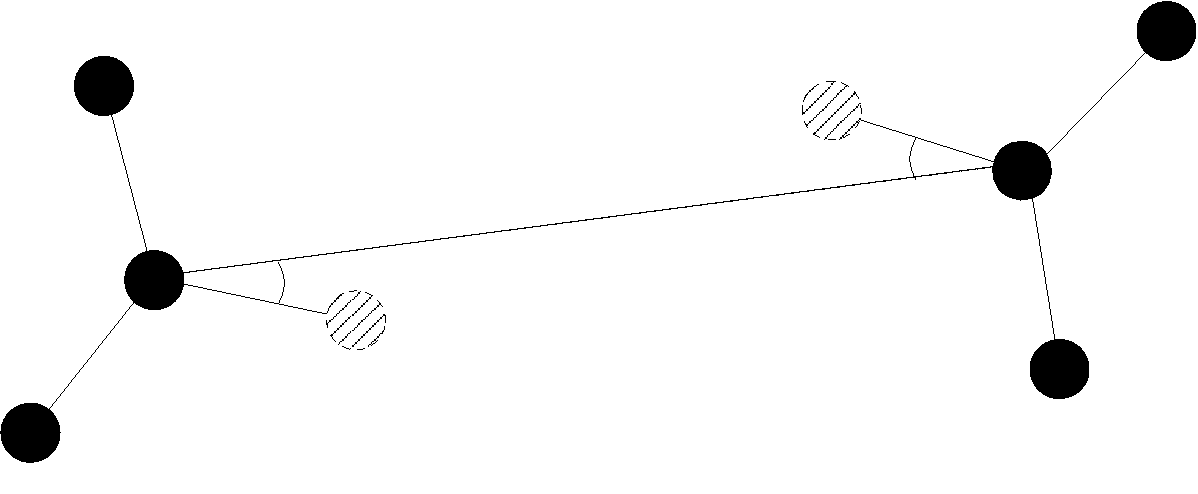
\includegraphics[height=8em]{figures/hbond}
\end{center}

specifies a 12-10 Lennard-Jones interaction with angular dependence
between particles of the types \var{type1} and
\var{type2}. These two particles need two bonded partners oriented in a symmetric way. They define an orientation for the central particle. The purpose of using bonded partners is to avoid dealing with torques, therefore the interaction does *not* need the ROTATION feature. The angular part of the potential minimizes the system when the two central beads are oriented along the vector formed by these two particles. The shaded beads on the image are virtual particles that are formed from the orientation of the bonded partners, connected to the central beads. They are used to define angles. The potential is of the form
\begin{equation}
  U(r_{ik},\theta_{jik},\theta_{ikn})=\epsilon\left[5\left(\frac{\sigma}r\right)^{12}-6\left(\frac{\sigma}{r}\right)^{10}\right]\cos^2\theta_{jik}\cos^2\theta_{ikn},
\end{equation}
where $r_{ik}$ is the distance between the two central beads, and each angle defines the orientation between the direction of a central bead (determined from the two bonded partners) and the vector $\mathbf{r_{ik}}$. Note that the potential is turned off if one of the angle is more than $\pi/2$. This way we don't end up creating a minimum for an anti-parallel configuration.

Unfortunately, the bonded partners are not seeked dynamically. One has to keep track of the relative positions of the particle IDs. This can be done by setting the parameters \var{b1_a}, \var{b1_b}, \var{b2_a}, and \var{b2_b}. Say the first bead \var{type1} has particle ID \var{n}, then one should set the simulation such as its two bonded partners have particle IDs \var{n+b1_a} and \var{n+b1_b}, respectively. On a linear chain, for example, one would typically have \var{b1_a=1} and \var{b1_b=-1} such that the central bead and its two bonded partners have position IDs \var{n}, \var{n+1}, and \var{n-1}, respectively. This is surely not optimized, but once the simulation is set correctly the algorithm is very fast. 

The force can be capped using \lit{inter ljangleforcecap}. It might turn out to be useful in some cases to keep this capping during the whole simulation. This is due to the very sharp angular dependence for small distance, compared to $\sigma$. Two beads might come very close to each other while having unfavorable angles such that the interaction is turned off. Then a change in the angle might suddenly turn on the interaction and the system will blow up (the potential is so steep that one would need extremely small time steps to deal with it, which is not very clever for such rare events). 

For instance, when modeling hydrogen bonds (N-H...O=C), one can avoid simulating hydrogens and oxygens by using this potential. This comes down to implementing a HBond potential between N and C atoms. 

NOTE : contribution to the pressure is not yet implemented.

\subsection{Smooth step interaction}
\index{smooth-step interaction|mainindex}
\index{interactions!smooth-step|mainindex}
\begin{essyntax}
  inter \var{type1} \var{type2}
  smooth-step \var{\sigma_1} \var{n} \var{\epsilon} \var{k_0}
  \var{\sigma_2} \var{r_\mathrm{cut}}
  \begin{features}
    \required{SMOOTH_STEP}
  \end{features}
\end{essyntax}
This defines a smooth step interaction between particles of the
types \var{type1} and \var{type2}, for which the potential is
\begin{equation}
  V(r)= \left(\var{\sigma_1}/d\right)^\var{n} + \epsilon/(1 + \exp\left[2k_0 (r - \sigma_2)\right])
\end{equation}
for $r<r_\mathrm{\var{cut}}$, and $V(r)=0$ elsewhere. With $n$ around 10, the
first term creates a short range repulsion similar to the Lennard-Jones
potential, while the second term provides a much softer repulsion. This
potential therefore introduces two length scales, the range of the first term,
$\sigma_1$, and the range of the second one, $\sigma_2$, where in general
$\sigma_1<\sigma_2$.

\subsection{BMHTF potential}
\index{BMHTF interaction|mainindex}
\index{interactions!BMHTF|mainindex}
\begin{essyntax}
  inter \var{type1} \var{type2}
  bmhtf-nacl \var{A} \var{B} \var{C} \var{D} \var{\sigma} \var{r_\mathrm{cut}}
  \begin{features}
    \required{BMHTF_NACL}
  \end{features}
\end{essyntax}
This defines an interaction with the {\em short-ranged part} of the
Born-Meyer-Huggins-Tosi-Fumi potential between particles of the types
\var{type1} and \var{type2}, which is often used to simulate NaCl
crystals. The potential is defined by:
\begin{equation}
  V(r)= \var{A}\exp\left[\var{B}(\var{\sigma} - \var{r})\right] -
  \var{C} \var{r}^{-6} - \var{D} \var{r}^{-8} + \epsilon_\mathrm{shift},
\end{equation}
where $\epsilon_\mathrm{shift}$ is chosen such that
$V(\var{r_\mathrm{cut}})=0$. For $r\ge \var{r_\mathrm{cut}}$, the
$V(r)=0$.

For NaCl, the parameters should be chosen as follows:

\begin{tabular}{r|l|l|l|l|l}
  types & \var{A} (\unitfrac{kJ}{mol}) & \var{B} ($\unit{\AA^{-1}}$) &
  \var{C} ($\unit{\AA^6}$\unitfrac{kJ}{mol}) & \var{D}
  $\unit{\AA^8}$\unitfrac{kJ}{mol} & \var{\sigma} (\unit{\AA}) \\
  \hline
  Na-Na & 25.4435 & 3.1546 &  101.1719 &    48.1771 & 2.34 \\
  Na-Cl & 20.3548 & 3.1546 &  674.4793 &   837.0770 & 2.755 \\
  Cl-Cl & 15.2661 & 3.1546 & 6985.6786 & 14031.5785 & 3.170 \\
\end{tabular}

The cutoff can be chosen relatively freely because the potential
decays fast; a value around 10 seems reasonable.

In addition to this short ranged interaction, one needs to add a Coulombic,
long--ranged part. If one uses elementary charges, \ie a charge of $q=+1$ for
the Na--particles, and $q=-1$ for the Cl--particles, the corresponding prefactor
of the Coulomb interaction is $\approx 1389.3549 \AA\,kJ/mol$.

\subsection{Morse interaction}
\index{Morse interaction|mainindex}
\index{interactions!Morse|mainindex}

\begin{essyntax}
  inter \var{type1} \var{type2} morse
  \var{\epsilon} \var{\alpha} \var{r_\mathrm{min}} \var{r_\mathrm{cut}}
  \begin{features}
    \required{MORSE}
  \end{features}
\end{essyntax}
This defines an interaction using the Morse potential between particles of the
types \var{type1} and \var{type2}. It serves similar purposes as the
Lennard-Jones potential, but has a deeper minimum, around which it is harmonic.
This models the potential energy in a diatomic molecule.  This potential allows
capping the force using {\tt inter morseforcecap}, see
section~\ref{sec:forcecap}.

For $r < \var{r_\mathrm{cut}}$, this potential is given by
\begin{equation}
  V(r)=\var{\epsilon}\left(\exp\left[-2 \var{\alpha} \left(r - \var{r_\mathrm{min}}\right)\right]
    - 2\exp\left[-\alpha\left(r - r_\mathrm{min}\right)\right]\right) -
  \epsilon_\mathrm{shift},
\end{equation}
where \var{\epsilon_\mathrm{shift}} is again chosen such that
$V(\var{r_\mathrm{cut}})=0$. For $r\ge \var{r_\mathrm{cut}}$, the $V(r)=0$.

\subsection{Buckingham interaction}
\index{Buckingham interaction|mainindex}
\index{interactions!Buckingham|mainindex}

\begin{essyntax}
  inter \var{type1} \var{type2} buckingham
  \var{A} \var{B} \var{C} \var{D}
  \var{r_\mathrm{cut}} \var{r_\mathrm{discont}} \var{\epsilon_\mathrm{shift}}
  \begin{features}
    \required{BUCKINGHAM}
  \end{features}
\end{essyntax}
This defines a Buckingham interaction between particles of the types
\var{type1} and \var{type2}, for which the potential is given by
\begin{equation}
  V(r)= A\exp(-B r) - Cr^{-6} - Dr^{-4} + \var{\epsilon_\mathrm{shift}}
\end{equation}
for $\var{r_\mathrm{discont}} < r < \var{r_\mathrm{cut}}$. Below \var{r_\mathrm{discont}},
the potential is linearly continued towards $r=0$, similarly to force capping,
see below. Above $r=\var{r_\mathrm{cut}}$, the potential is $0$. This potential
allows capping the force using \lit{inter buckforcecap}, see
section~\ref{sec:forcecap}.

\subsection{Soft-sphere interaction}
\index{soft-sphere interaction|mainindex}
\index{interactions!soft-sphere|mainindex}

\begin{essyntax}
  inter \var{type1} \var{type2}
  soft-sphere \var{a} \var{n} \var{r_\mathrm{cut}} \var{r_\mathrm{offset}}
  \begin{features}
    \required{SOFT_SPHERE}
  \end{features}
\end{essyntax}
This defines a soft sphere interaction between particles of the types
\var{type1} and \var{type2}, which is defined by a single power law:
\begin{equation}
  V(r)=a\left(r-r_\mathrm{\var{offset}}\right)^{-n}
\end{equation}
for $r<\var{r_\mathrm{cut}}$, and $V(r)=0$ above. There is no shift
implemented currently, which means that the potential is discontinuous
at $r=\var{r_\mathrm{cut}}$. Therefore energy calculations should be
used with great caution.

\subsection{Gay-Berne interaction}
\index{Gay-Berne interaction|mainindex}
\index{interactions!Gay-Berne|mainindex}

\begin{essyntax}
  inter \var{type1} \var{type2} gay-berne
  \var{\epsilon_0} \var{\sigma_0} \var{r_\mathrm{cutoff}}
  \var{k1} \var{k2} \var{\mu} \var{\nu}
  \begin{features}
    \required{ROTATION}
  \end{features}
\end{essyntax}
This defines a Gay-Berne potential for prolate and oblate particles
between particles of the types \var{type1} and \var{type2}. The
Gay-Berne potential is an anisotropic version of the classic
Lennard-Jones potential, with orientational dependence of the range
\var{\sigma_0} and the well-depth \var{\epsilon_0}.

Assume two particles with orientations given by the unit vectors
$\mathbf{\hat{u}}_i$ and $\mathbf{\hat{u}}_j$ and intermolecular vector
$\mathbf{r} = r\mathbf{\hat{r}}$. If $r<r_\mathrm{\var{cut}}$, then the
interaction between these two particles is given by
\begin{equation}
  V(\mathbf{r}_{ij}, \mathbf{\hat{u}}_i, \mathbf{\hat{u}}_j) = 4
  \epsilon(\mathbf{\hat{r}}_{ij}, \mathbf{\hat{u}}_i,
  \mathbf{\hat{u}}_j) \left( \tilde{r}_{ij}^{-12}-\tilde{r}_{ij}^{-6}
  \right),
\end{equation}
otherwise $V(r)=0$. The reduced radius is
\begin{equation}
  \tilde{r}=\frac{r - \sigma(\mathbf{\hat{r}},
    \mathbf{\hat{u}}_i, \mathbf{\hat{u}}_j)+\sigma_0}{\sigma_0},
\end{equation}
\begin{equation}
  \sigma( \mathbf{\hat{r}}, \mathbf{\hat{u}}_i,
  \mathbf{\hat{u}}_j) = \sigma_{0} \left\{ 1 - \frac{1}{2} \chi \left[
      \frac{ \left( \mathbf{\hat{r}} \cdot \mathbf{\hat{u}}_i +
          \mathbf{\hat{r}} \cdot \mathbf{\hat{u}}_j \right)^{2} }
      {1 + \chi \mathbf{\hat{u}}_i \cdot \mathbf{\hat{u}}_j } +
      \frac{ \left( \mathbf{\hat{r}} \cdot \mathbf{\hat{u}}_i -
          \mathbf{\hat{r}} \cdot \mathbf{\hat{u}}_j \right)^{2} }
      {1 - \chi \mathbf{\hat{u}}_i \cdot \mathbf{\hat{u}}_j}
    \right] \right\}^{-\frac{1}{2}}
\end{equation}
and
\begin{multline}
  \epsilon(\mathbf{\hat{r}}, \mathbf{\hat{u}}_i,
  \mathbf{\hat{u}}_j) = \\
  \epsilon_0 \left( 1- \chi^{2}(\mathbf{\hat{u}}_i
    \cdot \mathbf{\hat{u}}_j) \right)^{-\frac {\nu}{2}} \left[1-\frac
    {\chi'}{2} \left( \frac { (\mathbf{\hat{r}} \cdot
        \mathbf{\hat{u}}_i+ \mathbf{\hat{r}} \cdot
        \mathbf{\hat{u}}_j)^{2}} {1+\chi' \, \mathbf{\hat{u}}_i \cdot
        \mathbf{\hat{u}}_j }+ \frac {(\mathbf{\hat{r}} \cdot
        \mathbf{\hat{u}}_i-\mathbf{\hat{r}} \cdot
        \mathbf{\hat{u}}_j)^{2}} {1-\chi' \, \mathbf{\hat{u}}_i \cdot
        \mathbf{\hat{u}}_j } \right) \right]^{\mu}.
\end{multline}
The parameters $\chi = \left(k_1^{2} - 1\right)/\left(k_1^{2} +
  1\right)$ and $\chi' = \left(k_2^{1/\mu} -
  1\right)/\left(k_2^{1/\mu} + 1\right)$ are responsible for the
degree of anisotropy of the molecular properties.  \var{k_1} is the
molecular elongation, and \var{k_2} is the ratio of the potential well
depths for the side-by-side and end-to-end configurations.  The
exponents \var{\mu} and \var{\nu} are adjustable parameters of the
potential.  Several Gay-Berne parametrizations exist, the original one
being $\var{k_1} = 3$, $\var{k_2} = 5$, $\var{\mu} = 2$ and $\var{\nu}
= 1$.

\subsection{Tabulated interaction}
\index{tabulated interaction|mainindex}
\index{interactions!tabulated|mainindex}
\label{sec:tabnonbonded}

\begin{essyntax}
  inter \var{type1} \var{type2} tabulated \var{filename}%
  \begin{features}
    \required{TABULATED}
  \end{features}
\end{essyntax}

This defines an interaction between particles of the types \var{type1} and
\var{type2} according to an arbitrary tabulated pair potential. \var{filename}
specifies a file which contains the tabulated forces and energies as a function
of the separation distance. The tabulated potential allows capping the force
using {\tt inter tabforcecap}, see section~\ref{sec:forcecap}.

At present the required file format is simply an ordered list separated by
whitespace. The data reader first looks for a {\tt \#} character and begins
reading from that point in the file. Anything before the {\tt \#} will be
ignored.

The first three parameters after the {\tt \#} specify the number of data points
$N_\mathrm{points}$ and the minimal and maximal tabulated separation distances
$r_\mathrm{min}$ and $r_\mathrm{max}$. The number of data points obviously should
be an integer, the two other can be arbitrary positive doubles. Take care when
choosing the number of points, since a copy of each lookup table is kept on each
node and must be referenced very frequently. The maximal tabulated separation
distance also acts as the effective cutoff value for the potential.

The remaining data in the file should consist of n data triples $r$, $F(r)$ and
$V(r)$. $r$ gives the particle separation, $V(r)$ specifies the interaction
potential, and $F(r)= -V'(r)/r$ the force (note the factor $1/r$!). The values
of $r$ are assumed to be equally distributed between $r_\mathrm{min}$ and
$r_\mathrm{max}$ with a fixed distance of
$(r_\mathrm{max}-r_\mathrm{min})/(N_\mathrm{points}-1)$; the distance values $r$ in
the file are ignored and only included for human readability.

\subsection{Capping the force during warmup}
\label{sec:forcecap}

\begin{essyntax}
  \variant{1} inter ljforcecap \var{F_\mathrm{max}}
  \variant{2} inter morseforcecap \var{F_\mathrm{max}}
  \variant{3} inter buckforcecap \var{F_\mathrm{max}}
  \variant{4} inter tabforcecap \var{F_\mathrm{max}}
  \begin{features}
    \required[\variant{1}]{LENNARD_JONES}
    \required[\variant{2}]{MORSE}
    \required[\variant{3}]{BUCKINGHAM}
    \required[\variant{4}]{TABULATED}
  \end{features}  
\end{essyntax}

Non-bonded interactions are often used to model the hard core
repulsion between particles. Most of the potentials in the section are
therefore singular at zero distance, and forces usually become very
large for distances below the particle size. This is not a problem
during the simulation, as particles will simply avoid overlapping.
However, creating an initial dense random configuration without
overlap is often difficult.

By artificially capping the forces, it is possible to simulate a
system with overlaps. By gradually raising the cap value
\var{F_\mathrm{max}}, possible overlaps become unfavorable, and the
system equilibrates to a overlap free configuration.

This command will cap the force to \var{F_\mathrm{\var{max}}}, \ie for
particle distances which would lead to larger forces than
\var{F_\mathrm{max}}, the force remains at \var{F_\mathrm{max}}.
Accordingly, the potential is replaced by replaced by $r
\var{F_\mathrm{max}}$. Particles placed exactly on top of each other
will be subject to a force of magnitude \var{F_\mathrm{max}} along
the first coordinate axis.

The force capping is switched off by setting $\var{F_\mathrm{max}}=0$.
Note that force capping always applies to all interactions of the
corresponding type (\eg all Lennard-Jones interactions) regardless of
the particle types.

\section{Bonded interactions}
\label{sec:inter-bonded}
\index{bonded interactions|mainindex}
\index{interactions!bonded|mainindex}

\begin{essyntax*}
  inter \var{bondid}
  \opt{\var{interaction}}
  \opt{\var{parameters}}
\end{essyntax*}

\index{bonded interaction type id} Bonded interactions are identified
by their \emph{bonded interaction type identificator} \var{bondid},
which is a non-negative integer.  The \lit{inter} \var{bondid} command
is used to specify the type and parameters of a bonded interaction,
which applies to all particles connected explicitely by this bond
using the \keyword{part} command (see section \vref{tcl:part}).
Therefore, defining a bond between two particles always involves two
steps: defining the interaction and applying it. Assuming that two
particles with ids 42 and 43 already exist, one can create \eg a
FENE-bond between them using
\begin{tclcode}
  inter 1 fene 10.0 2.0
  part 42 bond 1 43
\end{tclcode}
If a FENE-bond with the same interaction parameters is required between several
particles (\eg in a simple chain molecule), one can use the sampe type \var{id}:
\begin{tclcode}
  inter 1 fene 10.0 2.0
  part 42 bond 1 43; part 43 bond 1 44 
\end{tclcode}

Bonds can have more than just two bond partners. For the \keyword{inter} command
that does not play a role as it only specifies the parameters, only when
applying the bond using the \keyword{bond} particle, the number of involved
particles plays a role. The number of involved particles and their order, if
important, is nevertheless specified here for completeness.

\subsection{FENE bond}
\index{FENE bond|mainindex}
\index{interactions!FENE|mainindex}

\begin{essyntax}
  inter \var{bondid}
  fene
  \var{K} \var{\Delta r_\mathrm{max}} \opt{\var{r_0}}
\end{essyntax}
This creates a bond type with identificator \var{bondid} with a
FENE (finite extension nonlinear expander) interaction. This is a
rubber-band-like, symmetric interaction betweeen two particles with
prefactor \var{K}, maximal stretching \var{\Delta r_\mathrm{max}} and
equilibrium bond length \var{r_0}.  The bond potential diverges at a
particle distance $r=\var{r_0}-\var{\Delta r_\mathrm{max}}$ and
$r=\var{r_0}+\var{\Delta r_\mathrm{max}}$. It is given by
\begin{equation}
  V(r) = -\frac{1}{2} \var{K} \var{\Delta r_\mathrm{max}}^2\ln \left[ 1 - \left(
      \frac{r-\var{r_0}}{\var{\Delta r_\mathrm{max}}} \right)^2 \right].
\end{equation}

\subsection{Harmonic bond}
\index{harmonic bond|mainindex}
\index{interactions!harmonic|mainindex}

\begin{essyntax}
  inter \var{bondid}
  harmonic \var{K} \var{R}
\end{essyntax}
This creates a bond type with identificator \var{bondid} with a
classical harmonic potential. It is a symmetric interaction between two
particles. The potential is minimal at particle distance $r=R$, and the
prefactor is $K$. It is given by
\begin{equation}
  V(r) = \frac{1}{2} K \left( r - R \right)^2
\end{equation}

\subsection{Subtracted Lennard-Jones bond}
\index{subtracted Lennard-Jones bond|mainindex}
\index{interactions!subtracted Lennard-Jones|mainindex}

\begin{essyntax}
  inter \var{bondid}
  subt_lj
  \var{reserved} \var{R}
\end{essyntax}
This creates a ``bond'' type with identificator \var{bondid}, which
acts between two particles and actually subtracts the Lennard-Jones interaction
between the involved particles.  The first parameter, \var{reserved} is a dummy
just kept for compatibility reasons. The second parameter, \var{R}, is used as a
check: if any bond length in the system exceeds this value, the program
terminates. When using this interaction, it is worthwhile to consider
capping the Lennard-Jones potential appropriately so that round-off errors can
be avoided.

This interaction is useful when using other bond potentials which already
include the short--ranged repulsion. This often the case for force fields or in
general tabulated potentials.

\subsection{Rigid bonds}
\index{rigid bond|mainindex}
\index{interactions!rigid bond|mainindex}
\index{RATTLE}

\begin{essyntax}
  inter \var{bondid}
  rigid_bond
  \var{constrained_bond_distance} \var{positional_tolerance} 
  \var{velocity_tolerance}
\end{essyntax}
\todo{Docs}

\subsection{Bond-angle interactions}
\index{bond-angle interactions|mainindex}
\index{interactions!bond-angle|mainindex}
\label{sec:angle}

\begin{essyntax}
  inter \var{bondid}
  angle \var{K} \opt{\var{\phi_0}}
  \begin{features}
    \required{BOND_ANGLE_HARMONIC, BOND_ANGLE_COSINE or BOND_ANGLE_COSSQUARE}
  \end{features}
\end{essyntax}

This creates a bond type with identificator \var{bondid}
with an angle dependent potential. This potential is defined between
three particles. The particle for which the bond is created, is the
central particle, and the angle $\phi$ between the vectors from this
particle to the two others determines the interaction.  \var{K} is the
bending constant, and the optional parameter \var{phi_0} is the
equilibirum bond angle in radian ranging from 0 to $\pi$.  If this
parameter is not given, it defaults to $\var{\phi_0} = \pi$, which
corresponds to a stretched configuration. For example, for a bond
defined by
\begin{code}
  part \$p_2 bond 4 \$p_1 \$p_3
\end{code}
the minimal energy configurations are the following:
\begin{center}
  \setlength{\unitlength}{3000sp}
  \begin{picture}(8381,2684)(1570,-5393)
    \thinlines
    \put(2701,-4561){\circle*{450}}
    \put(3601,-4561){\circle*{450}}
    \put(4501,-4561){\circle*{450}}
    \put(7021,-4561){\circle*{450}}
    \put(7921,-4561){\circle*{450}}
    \put(7921,-3661){\circle*{450}}
    \thicklines
    \put(2701,-4561){\line( 1, 0){1800}}
    \put(7021,-4561){\line( 1, 0){900}}
    \put(7921,-4561){\line( 0, 1){900}}
    \put(5761,-2831){\line( 0,-1){2500}}

    \put(2701,-5191){\makebox(0,0)[b]{$p_1$}}
    \put(3601,-5191){\makebox(0,0)[b]{$p_2$}}
    \put(4501,-5191){\makebox(0,0)[b]{$p_3$}}
    \put(7021,-5191){\makebox(0,0)[b]{$p_1$}}
    \put(8371,-3751){\makebox(0,0)[b]{$p_3$}}
    \put(7921,-5191){\makebox(0,0)[b]{$p_2$}}
    \put(7921,-2941){\makebox(0,0)[b]{\keyword{inter 4 angle 1.0 [expr [PI]/2]}}}
    \put(3601,-2941){\makebox(0,0)[b]{\keyword{inter 4 angle 1.0 [PI]}}}
  \end{picture}%
\end{center}

For the potential acting between the three particles, different choices are
possible, which have to be activated in \texttt{myconfig.h}
\begin{itemize}
\item Harmonic bond angle potential (requires feature BOND_ANGLE_HARMONIC):\\
  A classical harmonic potential,
  \begin{equation}
    V(\phi) = \frac{K}{2} \left(\phi - \phi_0\right)^2.
  \end{equation}
  Unlike the two following variants, this potential has a kink at
  $\phi=\phi_0+\pi$ and accordingly a discontinuity in the force, and should
  therefore be used with caution.
\item Cosine bond angle potential (requires feature BOND_ANGLE_COSINE):\\
  \begin{equation}
    V(\alpha) = K \left[1 - \cos(\phi - \phi0)\right]
  \end{equation}
  Around $\phi_0$, this potenial is close to a harmonic one (both are
  $1/2(\phi-\phi_0)^2$ in leading order), but it is periodic and smooth for all
  angles $\phi$.
\item Cosine square bond angle potential (requires feature
  BOND_ANGLE_COSSQUARE):\\
  \begin{equation}
    V(\alpha) = \frac{K}{2} \left[\cos(\phi) - \cos(\phi_0)\right]^2
  \end{equation}
  This form is used for example in the GROMOS96 force field. The potential is
  $1/8(\phi-\phi_0)^4$ around $\phi_0$, and therefore much flatter than the
  two potentials before.
\end{itemize}

\subsection{Dihedral interactions}
\index{dihedral interactions|mainindex}
\index{interactions!dihedral|mainindex}
\label{sec:dihedral}

\begin{essyntax}
  inter \var{bondid} dihedral \var{n} \var{K} \var{p}
\end{essyntax}

This creates a bond type with identificator \var{bondid}
with a dihedral potential, \ie a four-body-potential. In the following,
let the particle for which the bond is created be particle $p_2$, and
the other bond partners $p_1$, $p_3$, $p_4$, in this order, \ie
\lit{part $p_2$ bond bondid $p_1$ $p_3$ $p_4$}. Then, the
dihedral potential is given by
\begin{equation}
  V(\phi) = \var{K}\left[1 - \cos(\var{n}\phi - \var{p})\right],
\end{equation}
where \var{n} is the multiplicity of the potential (number of minimas)
and can take any integer value (typically from 1 to 6), $p$ is a phase
parameter and \var{K} is the bending constant of the potential. $\phi$
is the dihedral angle between the particles defined by the particle
quadrupel $p_1$, $p_2$, $p_3$ and $p_4$, \ie the angle between the
planes defined by the particle triples $p_1$, $p_2$ and $p_3$ and
$p_2$, $p_3$ and $p_4$:
\begin{center}
  \includegraphics[height=8em]{figures/dihedral-angle}
\end{center}
Together with appropriate Lennard-Jones interactions, this potential
can mimic a large number of atomic torsion potentials.

If you enable the feature OLD_DIHEDRAL, then the old, less
general form of the potential is used:
\begin{equation}
  V(\phi) = \var{K}\left[1 + \var{p}\,\cos(\var{n}\phi)\right],
\end{equation}
where $p$ is rather a phase factor and can only take values $p=\pm 1$.

\subsection{Tabulated bond interactions}
\index{tabulated bond interactions|mainindex}
\index{interactions!tabulated bond|mainindex}

\begin{essyntax}
    \variant{1} inter \var{bondid}
    tabulated bond \var{filename}
    \variant{2} inter \var{bondid}
    tabulated angle \var{filename}
    \variant{3} inter \var{bondid}
    tabulated dihedral \var{filename}
\end{essyntax}

This creates a bond type with identificator \var{bondid} with a
two-body bond length (\variant{1}), three-body angle (\variant{2}) or four-body
dihedral (\variant{3}) tabulated potential. The tabulated forces and energies
have to be provided in a file \var{filename}, which is formatted identically as
the files for non-bonded tabulated potentials (see
section\ref{sec:tabnonbonded}).

The potential is calculated as follows:
\begin{itemize}
\item Variant~\variant{1} is a two body interaction depending on the distance of
  two particles. The force acts in the direction of the connecting vector
  between the particles. The bond breaks above the tabulated range, but for
  distances smaller than the tabulated range, a linear extrapolation based on
  the first two tabulated force values is used.
\item Variant~\variant{2} is a three-body angle interaction similar to the
  \texttt{angle} potential (see section~\ref{sec:angle}).  It is assumed that
  the potential is tabulated for all angles between 0 and $ \pi $, where 0
  corresponds to a stretched polymer, and just as for the tabulated pair
  potential, the forces are scaled with the inverse length of the connecting
  vectors. The force on particles $p_1$ and $p_3$ (in the notation of
  section~\ref{sec:angle}) acts perpendicular to the connecting vector between
  the particle and the center particle $p_2$ in the plane defined by the three
  particles. The force on the center particle $p_2$ balances the other two
  forces.
\item Variant~\variant{3} tabulates a torsional dihedral angle potential (see
  section~\ref{sec:dihedral}). It is assumed that the potential is tabulated for
  all angles between 0 and $2\pi$. \em{This potential is not tested yet! Use on
    own risk, and please report your findings and eventually necessary fixes.}
\end{itemize}

\subsection{Virtual bonds}

\begin{essyntax}
  inter \var{bondid} virtual_bond
\end{essyntax}

This creates a virtual bond type with identificator \var{bondid}, \ie
a pair bond without associated potential or force. It can used to specify
topologies and for some analysis that rely on bonds, or \eg for bonds that
should be displayed in VMD.

\section{Coulomb interaction}
\label{sec:inter-electrostatics}
\index{Coulomb interactions|mainindex}
\index{interactions!Coulomb|mainindex}

Electrostatic interactions are very computation time-intensive. \es{} features
some state-of-the-art algorithms to deal with these interactions as efficiently
as possible, but almost all of them require some knowledge to use them properly.
Uneducated use can result in completely unphysical simulations.

\begin{essyntax}
  \variant{1} inter coulomb 0.0
  \variant{2} inter coulomb \opt{\var{l_B} \var{method}} \opt{\var{parameters}}
  \variant{3} inter coulomb
\end{essyntax}

This command defines how \es deals with electrostatic interactions.

Variant \variant{1} completely disables Coulomb interactions hence
deactivating the electrostatic subsystem, while variant \variant{2}
sets up one of the methods described below to treat electrostatic
interactions. \var{l_B} denotes the Bjerrum length, which measures the
strength of the electrostatic interaction.  For a pair of particles at
distance $r$ with charge $q$ each, the interaction is given by
\begin{equation}
  U^C(r)=l_B k_B T\frac{q^2}{r}.
\end{equation}
Using the electrostatic interaction also requires to assign charges to the
particles. This is done using the \texttt{part} command to set the charge
\texttt{q}, \eg

\begin{tclcode}
  inter coulomb 1.0 p3m tune accuracy 1e-4
  part 0 q 1.0; part 1 q -1.0
\end{tclcode}

Variant \variant{3} returns the current parameters of the coulomb
interaction as a tcl-list using the same syntax as used to setup the
method, \eg
\begin{tclcode}
  {coulomb 1.0 p3m 7.75 8 5 0.1138 0.0}
  {coulomb epsilon 0.1 n_interpol 32768 mesh_off 0.5 0.5 0.5}
\end{tclcode}

\subsection{P3M}
\index{P3M method|mainindex}
\index{interactions!P3M|mainindex}

\begin{essyntax}
  inter coulomb p3m \var{r_\mathrm{cut}} \var{mesh} \var{cao} \var{alpha}
\end{essyntax}

Activates the P3M method to handle the Coulomb
interaction
\begin{equation}
  U^{C-P3M} = \ell_B k_B T \frac{q_1 q_2}{r}
\end{equation}

Here $\ell_B = e_o^2 / (4 \pi \epsilon k_B T)$ is the Bjerrum length.
Make sure that you know the relevance of the P3M parameters before
using P3M! If you are not sure, read the following references
\cite{ewald21,hockney88,kolafa92,deserno98,deserno98a,deserno00,deserno00a}.

\subsubsection{Tuning P3M}
\begin{essyntax}
  inter coulomb p3m \alt{tune \asep tunev2}
  accuracy \var{accuracy}\\
  \opt{r_cut \var{r_\mathrm{cut}}}
  \opt{mesh \var{mesh}}
  \opt{cao \var{cao}}
  \opt{alpha \var{\alpha}}
\end{essyntax}

Make sure you know how to tune p3m parameters before using the
automatic tuning feature.

The function utilizes the analytic expression of the error estimate
for the P3M method in the book of Hockney and Eastwood \cite[eqn
8.23]{hockney88} in order to obtain the rms error in the force for a
system of N randomly distributed particles in a cubic box.  For the
real space error the estimate of Kolafa and Perram\cite{kolafa92} is
used.

The two tuning methods follow different methods for determining the
optimal parameter. While the \keyword{tune} version simply tests
different values on a grid in the parameter space, the
\keyword{tunev2} version uses a bisection to determine the optimal
parameters. In general, for small systems the \keyword{tune} version
is faster, while for large systems \keyword{tunev2} is faster. The
results of \keyword{tunev2} are always at least as good as the
parameters achievable from the \keyword{tune} version, and normally
the obtained accuracy is much closer to the desired value.

During execution the tuning routines report the parameter sets tested,
the corresponding k-space and real-space errors and timings needed for
force calculations (the setmd variable \var{timings} controls the
number of test force calculations). Since the error depends on
\var{r_\mathrm{cut}}/\var{box\_l} and \var{\alpha}\var{box\_l} the
output is given in these units.

Note that any previous settings of \var{r_\mathrm{cut}}, \var{cao} and
\var{mesh} will be remembered. So if you want to retune your
electrostatics, \eg after a major system change, you should use
\begin{code}
inter coulomb \var{l_B} p3m tune accuracy \var{acc} r_cut 0 mesh 0 cao 0
\end{code}

Some additional p3m parameters have preset value
\begin{tclcode}
 epsilon = metallic
\end{tclcode}
The dielectric constant of the surrounding medium, metallic
(i.e.infinity) or some finite positive number.
\begin{tclcode}
 n_interpol = 32768
\end{tclcode}
Number of interpolation points for the charge assignment function.
When this is set to 0, interpolation is turned off.
\begin{tclcode}
 mesh_off = 0.5 0.5 0.5
\end{tclcode}
Offset of the first mesh point from the lower left corner of the
simulation box in units of the mesh constant. As soon as p3m is turned
on the additional parameters can be changed with:
\begin{code}
inter coulomb \var{parameter_name} \var{value}+
\end{code}


\subsection{Debye-H\"uckel potential}
\index{Debye-H\"uckel potential|mainindex}
\index{interactions!Debye-H\"uckel|mainindex}

\todo{How is the cutoff handled? Why is this not a normal short-raged
  potential?}
\begin{essyntax}
  inter coulomb dh \var{\kappa} \var{r_\mathrm{cut}}
\end{essyntax}

Defines the electrostatic potential by
\begin{equation}
  U^{C-DH} = \ell_B k_B T \frac{q_1 q_2 exp(-\kappa r)}{r}
\end{equation}

For $\kappa = 0$, this corresponds to the plain coulomb potential.

\subsection{MMM2D}
\index{MMM2D method|mainindex}
\index{interactions!MMM2D|mainindex}

\begin{essyntax}
 inter coulomb mmm2d \var{maximal\_pairwise\_error} \opt{\var{fixed\_far\_cutoff}}
\end{essyntax}
MMM2D coulomb method for systems with periodicity 1 1 0. Needs the
layered cell system. The performance of the method depends on the
number of slices of the cell system, which has to be tuned manually.
It is automatically ensured that the maximal pairwise error is smaller
than the given bound. The far cutoff setting should only be used for
testing reasons, otherwise you are more safe with the automatical
tuning. If you even don't know what it is, do not even think of
touching the far cutoff. For details on the MMM family of algorithms,
refer to appendix \vref{chap:mmm}.

\subsection{MMM1D}
\index{MMM1D method|mainindex}
\index{interactions!MMM1D|mainindex}

\begin{essyntax}
  \variant{1}
  inter coulomb mmm1d \var{switch\_radius}
  \opt{\var{bessel\_cutoff}} \var{maximal\_pairwise\_error}

  \variant{2}
  inter coulomb mmm1d tune \var{maximal\_pairwise\_error}
\end{essyntax}
MMM1D coulomb method for systems with periodicity 0 0 1. Needs the
nsquared cell system (see section \vref{sec:cell-systems}). The first
form sets parameters manually. The switch radius determines at which
xy-distance the force calculation switches from the near to the far
formula. If the Bessel cutoff is not explicitly given, it is
determined from the maximal pairwise error, otherwise this error only
counts for the near formula. The second, tuning form just takes the
maximal pairwise error and tries out a lot of switching radii to find
out the fastest one. If this takes too long, you can change the value
of the setmd variable \keyword{timings}, which controls the number of
test force calculations. For details on the MMM family of algorithms,
refer to appendix \vref{chap:mmm}.

\subsection{Maggs' method}
\index{Maggs' method|mainindex}
\index{interactions!Maggs' method|mainindex}

\begin{essyntax}
  inter coulomb
  maggs \var{f\_mass} \var{mesh} \var{field\_friction}
  \opt{yukawa \var{kappa} \var{r_\mathrm{cut}}}
\end{essyntax}

This is an implementation of the instantaneous 1/r Coulomb interaction
\begin{equation}
  U = \ell_B k_B T \frac{q_1 q_2}{r}
\end{equation}
as the potential of mean force between charges which are dynamically
coupled to a local electromagnetic field.

\begin{arguments}
\item[\var{f\_mass}] is the mass of the field degree of freedom and equals
  to the square root of the inverted speed of light.
\item[\var{mesh}] is the number of mesh points for the interpolation
  of the electromagnetic field.
\item[\var{field\_friction}] is the value of the friction coefficient
  for the transversal field degrees of freedom (reserved for future
  development).
\end{arguments}
Unphysical self--energies that arise as a result of the lattice
interpolation of charges, are corrected by a subtraction scheme based
either on the exact lattice Green's function or the combination of the
direct subtraction scheme plus the Yukawa subtraction scheme (second
method).

For the case of Yukawa screened simulation (second method) one has to
enter screening parameter \var{kappa} and the cut-off of the Yukawa
potential \var{r_\mathrm{cut}}.

\subsection{ELC}
\index{ELC method|mainindex}
\index{interactions!ELC method|mainindex}

\begin{essyntax}
  inter coulomb elc \var{maximal\_pairwise\_error} \var{gap\_size}
  \opt{\var{far\_cutoff}}
\end{essyntax}
This is a special procedure that converts a 3d method, \ie P3M at the
moment, to a 2d method, in computational order N. This is definitely
faster than MMM2D for larger numbers of particles (>400 at reasonable
accuracy requirements). The maximal pairwise error is the LUB error of
the force between any two charges without prefactors (see the papers).
The gap size gives the height of the empty region between the system
box and the neighboring artificial images (again, see the paper).
\es{} does not make sure that the gap is actually empty, this is the
users responsibility. The method will compute fine of the condition is
not fulfilled, however, the error bound will not be reached. Therefore
you should really make sure that the gap region is empty (e. g. by
constraints). The far cutoff finally is only intended for testing and
allows to directly set the cutoff. In this case, the maximal pairwise
error is ignored. The periodicity has to be set to 1 1 1 still, and
the 3d method has to be set to epsilon metallic, i.e.  metallic
boundary conditions. For details, see appendix \vref{chap:mmm}.

Make sure that you read the papers on ELC before using it !!!
\todo{references}

\section{Other interaction types}
\label{sec:inter-other}

\subsection{Fixing the center of mass}
\begin{essyntax}
  inter \var{typeid1} \var{typeid1} comfixed \var{flag}
\end{essyntax}
This interaction type applies a constraint on particles of type
\var{typeid1} such that during the integration the center of mass of
these particles is fixed. This is accomplished as follows: The sum of
all the forces acting on particles of type \var{typeid1} are
calculated. These include all the forces due to other interaction
types and also the thermostat. Next a force equal in magnitude, but in
the oppositte direction is applied on the particles. This force is
divided equally on all the particles of type \var{typeid1}, since
currently there is no mass concept in \es. Note that the syntax of the
declaration of comfixed interaction requires the same particle type to
be input twice. If different particle types are given in the input,
the program exits with an error message. \var{flag} can be set to 1
(which turns on the interaction) or 0 (to turn off the interaction).

\subsection{Pulling particles apart}
\begin{essyntax}
  inter \var{typeid1} \var{typeid2}
  comforce \var{flag} \var{dir} \var{force} \var{fratio}
\end{essyntax}
The comforce interaction type enables one to pull away particle groups
of two different types. It is mainly designed for pulling experiments
on bundles. Within a bundle of molecules of type number \var{typeid1}
lets mark one molecule as of type \var{typeid2}. Using comforce one
can apply a force such that t2 can be pulled away from the bundle. The
\var{comforce_flag} is set to 1 to turn on the interaction, and to 0
otherwise. The pulling can be done in two different directions. Either
parallel to the major axis of the bundle ($\var{dir} = 0$) or
perpendicular to the major axis of the bundle ($\var{dir} = 1$).
\var{force} is used to set the magnitude of the force.  \var{fratio}
is used to set the ratio of the force applied on particles of
\var{typeid1} vs. \var{typeid2}. This is useful if one has to keep the
total applied force on the bundle and on the target molecule the same.
A force of magnitude \var{force} is applied on \var{typeid2}
particles, and a force of magnitude (\var{force} * \var{fratio}) is
applied on \var{typeid1} particles.

%%% Local Variables:
%%% mode: latex
%%% TeX-master: "ug"
%%% End:

\chapter{Setting up the system}
\label{chap:setup}

\section{\texttt{setmd}: Setting global variables.}
\eslabel{setmd}

\begin{essyntax}
\variant{1} setmd \var{variable}
\variant{2} setmd \var{variable} \opt{\var{value}}+
\end{essyntax}
\todo{Explain '+' in intro.}

Variant \variant{1} returns the value of the \es global variable
\var{variable}, variant \variant{2} can be used to set the variable
\var{variable} to \var{value}. The following global variables can be
set:

%% List-environment for the description of the global variables
\newenvironment{globvar}{
  \begin{list}{}{
      \setlength{\rightmargin}{1em}
      \setlength{\leftmargin}{2em}
      \setlength{\partopsep}{0pt}
      \setlength{\topsep}{1ex}
      \setlength{\parsep}{0.5ex}
      \setlength{\listparindent}{-1em}
      \setlength{\labelwidth}{0.5em}
      \setlength{\labelsep}{0.5em}
      \renewcommand{\makelabel}[1]{%
        \index{##1@\texttt{##1} (global variable)|mainindex}%
        \index{global variables!\texttt{##1}|mainindex}%
        \texttt{##1}%
      }
    }
  }{
  \end{list}
}
\newcommand{\ro}{\emph{read-only}}

\todo{Better throw some out (\eg switches)?}
\todo{Missing: lattice_switch, dpd_tgamma, n_rigidbonds}
\todo{Which commands can be used to set the \emph{read-only}
  variables?}
\begin{globvar}
\item[box_l] (double[3]) Simulation box length.
  \todo{document what happens to the particles when \keyword{box_l} is
    changed!}
\item[cell_grid] (int[3], \ro) Dimension of the inner
  cell grid.
\item[cell_size] (double[3], \ro) Box-length of a cell.
\item[dpd_gamma] (double, \ro) Friction constant for the
  DPD thermostat.
\item[dpd_r_cut] (double, \ro) Cutoff for DPD thermostat.
\item[gamma] (double, \ro) Friction constant for the
  Langevin thermostat.
\item[integ_switch] (int, \ro) Internal switch which integrator to
  use.
\item[local_box_l] (int[3], \ro) Local simulation box length of the
  nodes.
\item[max_cut] (double, \ro) Maximal cutoff of real space
  interactions.
\item[max_num_cells] (int) Maximal number of cells for the link cell
  algorithm.  Reasonable values are between 125 and 1000, or for some
  problems (\var{n_total_particles} / \var{n_nodes}).
\item[max_seen_particle] (int, \ro) Maximal identity of a particle.
  \emph{This is in general not related to the number of particles!}
\item[max_range] (double, \ro) Maximal range of real space
  interactions: \var{max_cut} + \var{skin}.
\item[max_skin] (double, \ro) Maximal skin to be used for the link
  cell/verlet algorithm. This is the minimum of \var{cell_size} -
  \var{max_range}. \todo{???}
\item[min_num_cells] (int) \todo{???} Minimal number of cells for the
  link cell algorithm. Reasonable values range in $1e-6 N^2$ to $1e-7
  N^2$. In general just make sure that the Verlet lists are not
  incredibly large. By default the minimum is 0, but for the automatic
  P3M tuning it may be wise to larger values for high particle
  numbers.
\item[n_layers] (int, \ro) Number of layers in cell structure LAYERED
  (see section \vref{sec:cell-systems}).
\item[n_nodes] (int, \ro) Number of nodes.
\item[n_total_particles] (int, \ro) Total number of particles.
\item[n_particle_types] (int, \ro) Number of particle types that were
  used so far in the \keyword{inter} command (see chapter{tcl:inter}).
\item[node_grid] (int[3]) 3D node grid for real space domain
  decomposition (optional, if unset an optimal set is chosen
  automatically).
\item[nptiso_gamma0] (double, \ro)\todo{Docs missing.}
\item[nptiso_gammav] (double, \ro)\todo{Docs missing.}
\item[npt_p_ext] (double, \ro) Pressure for NPT simulations.
\item[npt_p_inst] (double) Pressure calculated during an
  NPT_isotropic integration.
\item[piston] (double, \ro) Mass off the box when using NPT_isotropic
  integrator.
\item[periodicity] (bool[3]) Specifies periodicity for the three
  directions. If the feature PARTIAL_PERIODIC is set, this variable
  can be set to (1,1,1) or (0,0,0) at the moment.  If not it is
  readonly and gives the default setting (1,1,1).\todo{Correct?}
\item[skin] (double) Skin for the Verlet list.
\item [temperature] (double, \ro) Temperature of the
  simulation.
\item[thermo_switch] (double, \ro) Internal variable which thermostat
  to use. 
\item[time] (double) The simulation time.
\item[time_step] (double) Time step for MD integration.
\item[timings] (int) Number of timing samples to take into account if
  set.\todo{???}
\item[transfer_rate] (int, \ro) Transfer rate for VMD connection. You
  can use this to transfer any integer value to the simulation from
  VMD.
\item[verlet_flag] (bool) Indicates whether the Verlet list will be
  rebuild. The program decides this normally automatically based on
  your actions on the data.
\item[verlet_reuse] (double) Average number of integration steps the
  verlet list has been re-used.
\end{globvar}

\section{\texttt{thermostat}: Setting up the thermostat}
\eslabel{thermostat}

\begin{essyntax}
  \variant{1} thermostat off
  \variant{2} theormstat \var{method} \opt{\var{parameter}}+
\end{essyntax}
\todo{Include docs from \texttt{thermostat.h}!}
Change thermostat settings.

\section{\texttt{nemd}: Setting up non-equilibrium MD}
\eslabel{nemd}

\begin{essyntax}
  \variant{1}nemd \var{method} \var{parameter} 
  \variant{2}nemd off
  \variant{3}nemd profile
  \variant{4}nemd viscosity
\end{essyntax}
\todo{Include docs from \texttt{nemd.h}!}
\todo{Put \texttt{nemd profile|viscosity} into \texttt{analyze}?}  
Use NEMD (Non Equilibrium Molecular Dynamics) to simulate a system
under shear.

\section{\texttt{cellsystem}: Setting up the cell system}
\label{sec:cell-systems}
\eslabel{cellsystem}

This section deals with the flexible particle data organization of
\es.  Due to different needs of different algorithms, \es is able to
change the organization of the particles in the computer memory,
according to the needs of the used algorithms. For details on the
internal organization, refer to section
\vref{sec:internal-particle-organization}.

\subsection{Domain decomposition}
\index{domain decomposition}
\begin{essyntax}
  cellsystem domain_decomposition \opt{-no_verlet_list}
\end{essyntax}
This selects the domain decomposition cell scheme, using Verlet lists
for the calculation of the interactions. If you specify
\keyword{-no_verlet_list}, only the domain decomposition is used, but
not the Verlet lists.

The domain decomposition cellsystem is the default system and suits
most applications with short ranged interactions. The particles are
divided up spatially into small compartments, the cells, such that the
cell size is larger than the maximal interaction range. In this case
interactions only occur between particles in adjacent cells. Since the
interaction range should be much smaller than the total system size,
leaving out all interactions between non-adjacent cells can mean a
tremendous speed-up. Moreover, since for constant interaction range,
the number of particles in a cell depends only on the density. The
number of interactions is therefore of the order N instead of order
$N^2$ if one has to calculate all pair interactions.

\subsection{N-squared}
\begin{essyntax}
  cellsystem nsquare 
\end{essyntax}
This selects the very primitive nsquared cellsystem, which calculates
the interactions for all particle pairs. Therefore it loops over all
particles, giving an unfavorable computation time scaling of $N^2$.
However, algorithms like MMM1D or the plain Coulomb interaction in the
cell model require the calculation of all pair interactions.

In a multiple processor environment, the nsquared cellsystem uses a
simple particle balancing scheme to have a nearly equal number of
particles per CPU, \ie $n$ nodes have $m$ particles, and $p-n$ nodes
have $m+1$ particles, such that $n*m+(p-n)*(m+1)=N$, the total number
of particles. Therefore the computational load should be balanced
fairly equal among the nodes, with one exception: This code always
uses one CPU for the interaction between two different nodes. For an
odd number of nodes, this is fine, because the total number of
interactions to calculate is a multiple of the number of nodes, but
for an even number of nodes, for each of the $p-1$ communication
rounds, one processor is idle.

E.g. for 2 processors, there are 3 interactions: 0-0, 1-1, 0-1.
Naturally, 0-0 and 1-1 are treated by processor 0 and 1, respectively.
But the 0-1 interaction is treated by node 1 alone, so the workload
for this node is twice as high. For 3 processors, the interactions are
0-0, 1-1, 2-2, 0-1, 1-2, 0-2. Of these interactions, node 0 treats 0-0
and 0-2, node 1 treats 1-1 and 0-1, and node 2 treats 2-2 and 1-2.

Therefore it is highly recommended that you use nsquared only with an
odd number of nodes, if with multiple processors at all. 

\subsection{Layered cell system}
\begin{essyntax}
  cellsystem layered \var{n_layers}
\end{essyntax}

This selects the layered cell system, which is specifically designed
for the needs of the MMM2D algorithm. Basically it consists of a
nsquared algorithm in x and y, but a domain decomposition along z, i.
e. the system is cut into equally sized layers along the z axis. The
current implementation allows for the cpus to align only along the z
axis, therefore the processor grid has to have the form 1x1xN.
However, each processor may be responsible for several layers, which
is determined by \var{n\_layers}, i. e. the system is split into
N*\var{n\_layers} layers along the z axis. Since in x and y direction
there are no processor boundaries, the implementation is basically
just a stripped down version of the domain decomposition cellsystem.

%%% Local Variables: 
%%% mode: latex
%%% TeX-master: "ug"
%%% End: 

\chapter{Running the simulation}
\label{chap:run}

\section{\texttt{integrate}: Running the simulation}
\newescommand{integrate}

\begin{essyntax}
  \variant{1} integrate \var{steps}
  \variant{2} integrate set \var{method} \opt{\var{parameter}}\dots
\end{essyntax}

\todo{Docs missing!}
\todo{Which integrators do exist?}

\section{\texttt{change_volume}: Changing the box volume}
\newescommand[change-volume]{change_volume}

\begin{essyntax}
  \variant{1} change_volume \var{V_\mathrm{new}} 
  \variant{2} change_volume \var{L_\mathrm{new}} \alt{x \asep y \asep z \asep xyz}
\end{essyntax}
Changes the volume of either a cubic simulation box to the new volume
\var{V_\mathrm{new}} or its given x-/y-/z-/xyz-extension to the new
box-length \var{L_\mathrm{new}}, and isotropically adjusts the
particles coordinates as well. The function returns the new volume of
the deformed simulation box.

\section{Stopping particles}
\newescommand{stopParticles}
\newescommand[stop-particles]{stop_particles}

\begin{essyntax}
  \variant{1} stopParticles
  \variant{2} stop_particles
\end{essyntax}
Halts all particles in the current simulation, setting their
velocities and forces to zero. Variant \variant{2} does not provide
feedback on the execution status.

\section{\texttt{velocities}: Setting the velocities}
\newescommand{velocities}
\begin{essyntax}
  velocities \var{v_\mathrm{max}} 
  \opt{start \var{pid}} 
  \opt{count \var{N}}
\end{essyntax}
Sets the velocities of the particles with particle IDs between
\var{pid} and $\var{pid}+\var{N}$ to a random vector with a length
less than \var{v_\mathrm{max}}, and returns the absolute value of the
total velocity assigned. By default, all particles are affected.

\section{\texttt{invalidate_system}}
\newescommand[invalidate-system]{invalidate_system}
\begin{essyntax}
  invalidate_system
\end{essyntax}
\todo{Documentation not up to date!}

Forces a system re-init which, among others, causes the integrator to
also update the forces at its beginning (instead of re-using the
values from the previous integration step).  This is particularly
necessary to ensure continuity after setting a checkpoint:
\texttt{integrate} - \texttt{set_checkpoint} - \texttt{integrate} has
only one call to \todo{???}???, while \texttt{read_checkpoint} -
\texttt{integrate} has two at the beginning of the 2nd integrate
(because loading a new system from disk typically requires
re-initializing the system), and since ??? also uses the thermostat
which in turn draws random numbers, the two situations do not end up
at the same segment of the random number sequence, all random events
will therefore slightly differ.  To prevent this, simply include a
call to invalidate_system upon setting the checkpoint (this is being
done automatically if using tcl_checkpoint_set and
tcl_checkpoint_read beginning with v1.1 of \es{}), because in that
case both scenarios will call ??? twice at the beginning of the second
integration phase thus having their random number sequences in total
sync.

\section{Parallel tempering}
\newescommand[parallel-tempering]{parallel_tempering}
\begin{essyntax}
  parallel_tempering::main
  -rounds \var{N}
  -swap \var{swap}
  -perform \var{perform}
  \opt{-init \var{init}}
  \opt{-values \var{\{T_i\}}}
  \opt{-connect \var{master}}
  \opt{-port \var{port}}
  \opt{-load \var{j_\mathrm{node}}}
  \opt{-resrate \var{N_\mathrm{reset}}}
  \opt{-info \var{info}}
\end{essyntax}

This command can be used to run a parallel tempering simulation. Since the simulation routines and
the calculation of the swap probabilities are provided by the user, the method is not limited to
sampling in the temperature space. However, we assume in the following that the sampled values are
temperatures, and call them accordingly. It is possible to use multiple processors via TCP/IP
networking, but the number of processors can be smaller than the number of temperatures.

\begin{arguments}
\item[\var{swap}] specifies the name of the routine calculating the
  swap probability for a system. The routine has to accept three
  parameters: the \var{id} of the system to evaluate, and two
  temperatures \var{T_1} and \var{T_2}. The routine should return a
  list containing the energy of the system at temperatures \var{T_1}
  and \var{T_2}, respectively.
\item[\var{perform}] specifies the name of the routine performing the
  simulation between two swap tries. The routine has to accept two
  parameters: the \var{id} of the system to propagate and the
  temperature \var{T} at which to run it. Return values are ignored.
\item[\var{init}] specifies the name of a routine initializing a
  system. This routine can for example create the particles, perform
  some intial equilibration or open output files.  The routine has to
  accept two parameters: the \var{id} of the system to initialize and
  its initial temperature \var{T}. Return values are ignored.
\item[\var{R}] specifies the number of swap trial rounds; in each
  round, neighboring temperatures are tried for swapping
  alternatingly, i.e. with four temperatures, The first swap trial
  round tries to swap $1\leftrightarrow 2$ and $3\leftrightarrow 4$,
  the second round $2\leftrightarrow 3$, and so on.
\item[\var{master}] the name of the host on which the
  parallel_tempering master node is running.
\item[\var{port}] the TCP/IP port on which the parallel_tempering
  master should listen. This defaults to 12000.
\item[\var{j_\mathrm{node}}] specifies how many systems to run per
  \es{}-instance. If this is more than 1, it is the user's
  responsibility to manage the storage of configurations, see below
  for examples.  This defaults to 1.
\item[\var{R_\mathrm{reset}}] specifies after how many swap trial
  rounds to reset the counters for the acceptance rate statistics.
  This defaults to 10.
\item[\var{info}] specifies which output the parallel tempering code
  should produce:
  \begin{itemize}
  \item[\texttt{none}] parallel tempering will be totally quiet,
    except for fatal errors
  \item[\texttt{comm}] information on client activities, such as
    connecting, is printed to stderr
  \item[\texttt{all}] print lots of information on swap energies and
    probabilities to stdout. This is useful for debugging and quickly
    checking the acceptance rates.
  \end{itemize}
  This defaults to \texttt{all}.
\end{arguments}

\subsubsection{Introduction}

The basic idea of parallel tempering is to run $N$ simulations with configurations $C_i$ in
parallel at different temperatures $T_1<T_2<\hdots<T_N$, and exchange configurations between
neighboring temperatures. This is done according to the Boltzmann rule, \ie the swap probability
for two configurations A and B at two different parameters $T_1$ and $T_2$ is given by
\begin{equation}
  \label{eq:ptacceptance}
  \min\left(1,\exp -\left[\beta(T_2)U_\text{A}(T_2) + \beta(T_1)U_\text{B}(T_1) -
    \beta(T_1)U_\text{A}(T_1) - \beta(T_2)U_\text{B}(T_2)\right]\right),
\end{equation}
where $U_C(T)$ denotes the potential energy of configuration $C$ at parameter $T$ and $\beta(T)$
the corresponding inverse temperature. If $T$ is the temperature, $U_C$ is indepedent of $T$, and
$\beta(T)=1/(k_BT)$. In this case, the swap probability reduces to the textbook result
\begin{equation}
  \min(1,\exp -\left[\left(1/T_2 - 1/T_1\right)\left(U_\text{A} - U_\text{B}\right)/k_B\right].
\end{equation}
However, $T$ can also be chosen to be any other parameter, for example the Bjerrum length, \ie the
the strength of the electrostatic interaction. In this case, $\beta(T)=\beta$ is a constant, but
the energy $U_C(T)$ of a configuration $C$ depends on $T$, and one needs the full
expression~\eqref{eq:ptacceptance}. \es{} always uses this expression.

In practice, one does not swap configurations, but temperatures, simply because exchanging
temperatures requires much less communication than exchanging the properties of all particles.

Th \es{} implementation of parallel tempering repeatedly propagates all configurations $C_i$ and
tries to swap neighboring temperatures. After the first propagation, the routine attempts to swap
temperatures $T_1$ and $T_2$, $T_3$ and $T_4$, and so on. After the second propagation, swaps are
attempted between temperatures $T_2$ and $T_3$, $T_4$ and $T_5$, and so on.  For the propagation,
parallel tempering relies on a user routine; typically, one will simply propagate the configuration
by a few 100 MD time steps.

\subsubsection{Details on usage and an example}

The parallel tempering code has to be loaded explicitely by {\tt source
  "scripts/parallel_tempering.tcl"} from the Espresso directory. To make use of the parallel
tempering tool, one needs to implement three methods: the propagation, the energy calculation and
an initialization routine for a configuration. A typical initialization routine will look roughly
like this:
\begin{verbatim}
proc init {id temp} {
  # create output files for temperature temp
  set f [open "out-$temp.dat" w]; close $f
  init_particle_positions
  thermostat langevin $temp 1.0
  equilibration_integration
  global config
  set config($id) "{[part]} [setmd time]"
}
\end{verbatim}
The last two lines are only necessary if each instance of \es{} handles more than one
configuration, \eg if you have 300 temperatures, but only 10 \es{} processes
(\ie {\tt -load 30}).  In this case, all
user provided routines need to save and restore the configurations. Saving the time is not
necessary because the simulation tine across swaps is not meaningful anyways; it is however
convenient for investigating the (temperature-)history of individual configurations.

A typical propagation routine accordingly looks like this
\begin{verbatim}
proc perform {id temp} {
  global config
  foreach p [lindex $config($id) 0] { eval part $p }
  setmd time [lindex $config($id) 1]
  thermostat langevin $temp 1.0
  set f [open "out-$temp.dat" a];
  integrate 1000
  puts $f "[setmd time] [analyze energy]"
  close $f
  set config($id) "{[part]} [setmd time]"
}
\end{verbatim}
Again, the saving and storing of the current particle properties in the config array are only
necessary if there is more than one configuration per process. In practice, one will rescale the
velocities at the beginning of perform to match the current temperature, otherwise the thermostat
needs a short time to equilibrate. The energies necessary to determine the swap probablility are
calculated like this:
\begin{verbatim}
proc swap {id temp1 temp2} {
  global config
  foreach p $config($id) { eval part $p }
  set epot [expr [analyze energy total] - [analyze energy kinetic]]
  return "[expr $epot/$temp1] [expr $epot/$temp2]"
}
\end{verbatim} % make emacs happy: $
Note that only the potential energy is taken into account. The temperature enters only indirectly
through the inverse temperature prefactor, see Eqn.~\eqref{eq:ptacceptance}.

The simulation is then started as follows. One of the processes runs the command
\begin{verbatim}
for {set T 0} {$T < 3} {set T [expr $T + 0.01]} {
    lappend temperatures $T }
parallel_tempering::main -load 30 -values $temperatures -rounds 1000 \
    -init init -swap swap -perform perform
\end{verbatim}
This command turns the \es instance executing it into the master part of the parallel tempering
simulation. It waits until a sufficient number of clients has connected. This are additional \es{}
instances, which are identical to the master script, except that they execute
\begin{verbatim}
parallel_tempering::main -connect $host -load 30 \
    -init init -swap swap -perform perform
\end{verbatim} % make emacs happy: $
Here, {\tt host} is a variable containing the TCP/IP hostname of the computer running the master
process. Note that the master process waits until enough processes have connected to start the
simulation. In the example, there are 300 temperatures, and each process, including the master
process, will deal with 30 of them. Therefore, 1 master and 9 slave processes are required. For a
typical queueing system, a starting routine could look like this:
\begin{verbatim}
master=
for h in $HOSTS; do
  if [ "$master" == "" ]; then
    ssh $h "cd run; ./pt_test.tcl"
    master=$h;
  else
    ssh $h "cd run; ./pt_test.tcl -connect $host"
  fi
done
\end{verbatim}
where {\tt pt_test.tcl} passes the {\tt -connect} option on to {\tt parallel_tempering::main}.

\subsubsection{Sharing data}

\begin{essyntax}
  parallel_tempering::set_shareddata \var{data}
\end{essyntax}

can be used at any time {\em by the master process} to specify additional data that is available on
all processes of the parallel_tempering simulation. The data is accessible from all processes as
{\tt parallel_tempering::shareddata}.

%%% Local Variables: 
%%% mode: latex
%%% TeX-master: "ug"
%%% End: 

\chapter{Analysis}
\label{chap:analysis}
\index{analysis}
\newescommand{analyze}

\todo{Intro: \lit{analyze} can measure observables, but also define
  topologies and store configurations}
\section{Measuring observables}

The \keyword{analyze}-command provides online-calculation of local and
global observables.

\todo{Missing: 
  \keyword{radial_density_map}, 
  \keyword{modes2d},
  \keyword{get_lipid_orients},
  \keyword{get_folded_positions},
  \keyword{bilayer_set},
  \keyword{bilayer_density_profile},
  \keyword{lipid_orient_order},
  \keyword{cell_gpb},
  \keyword{Vkappa}
}

\subsection{Minimal distances between particles}
\label{analyze:mindist}
\label{analyze:distto}
\analyzeindex{minimal particle distance}
\analyzeindex{particle distance}

\begin{essyntax}
  \variant{1} analyze mindist \opt{\var{type\_list\_a} \var{type\_list\_b}}
  \variant{2} analyze distto \var{pid}
  \variant{3} analyze distto \var{x} \var{y} \var{z}
\end{essyntax}

Variant \variant{1} returns the minimal distance between two particles
in the system. If the type-lists are given, then the minimal distance
between particles of only those types is determined.

\keyword{distto} returns the minimal distance of all particles to
particle \var{pid} (variant \variant{2}), or to the coordinates
(\var{x}, \var{y}, \var{z}) (Variant \variant{3}).

\subsection{Particles in the neighbourhood}
\label{analyze:nbhood}
\analyzeindex{particles in the neighbourhood}

\begin{essyntax}
 \variant{1} analyze nbhood \var{pid} \var{r\_catch}
 \variant{2} analyze nbhood \var{x} \var{y} \var{z}
 \var{r_catch}
\end{essyntax}
Returns a Tcl-list of the particle ids of all particles within a given
radius \var{r\_catch} around the position of the particle with number
\var{pid} in variant \variant{1} or around the spatial coordinate
(\var{x}, \var{y}, \var{z}) in variant \variant{2}.

\subsection{Particle distribution}
\label{analyze:distribution}
\analyzeindex{particle distribution}

\begin{essyntax}
  analyze distribution \var{part\_type\_list\_a} \var{part\_type\_list\_b}
  \opt{\var{rmin} \opt{\var{rmax} \opt{\var{rbins} 
        \opt{\var{log\_flag} \opt{\var{int\_flag}}}}}}
\end{essyntax}
Returns its parameters and the distance distribution of particles with
types specified in \var{part\_type\_list\_a} around particles with
types specified in \var{part\_type\_list\_b} with distances between
\var{rmin} and \var{rmax}, binned into \var{rbins} bins. The
bins are either equidistant (if $\var{log\_flag} = 0$) or
logarithmically equidistant (if $\var{log_flag} \geq 1$). If an
integrated distribution is required, use $\var{int_flag}=1$. The
distance is defined as the \emph{minimal} distance between a particle
of one group to any of the other group.

\minisec{Output format} 

The output corresponds to the blockfile format (see section
\vref{sec:structured-file-format}):
\begin{code}
\{ \var{parameters} \} 
\{ 
  \{ \var{r} \var{dist(r)} \} 
  \vdots 
\}
\end{code}

\subsection{Radial distribution function}
\label{analyze:rdf}
\label{analyze:<rdf>}
\analyzeindex{radial distribution function $g(r)$}

\begin{essyntax}
  analyze \alt{rdf \asep <rdf>} 
  \var{part\_type\_list\_a} \var{part\_type\_list\_b} 
  \opt{\var{rmin} \var{rmax} \var{rbins}}
\end{essyntax}
Returns its parameters and the radial distribution function (rdf) of
particles with types specified in \var{part\_type\_list\_a} around
particles with types specified in \var{part\_type\_list\_b}. The range
is given by \var{rmin} and \var{rmax} and is divided into
\var{rbins} equidistant bins.

\minisec{Output format}

The output corresponds to the blockfile format (see section
\vref{sec:structured-file-format}):
\begin{code}
\{ \var{parameters} \} 
\{ 
  \{ \var{r} \var{rdf(r)} \} 
  \vdots
\}
\end{code}

\subsection{Structure factor}
\label{analyze:structurefactor}
\analyzeindex{structure factor $S(q)$}

\begin{essyntax}
  analyze structurefactor \var{type} \var{order}
\end{essyntax}

Returns the spherically averaged structure factor $S(q)$ for particles
of a given type \var{type}. The $S(q)$ is calculated for all possible
wave vectors, $\frac{2\pi}{L} <= q <= \frac{2\pi}{L}\var{order}$. Do
not chose parameter \var{order} too large, becase the number of
calculations grows as $\var{order}^3$. 


\minisec{Output format} 

The output corresponds to the blockfile format (see section
\vref{sec:structured-file-format}):
\begin{code}
\{ \var{q\_value} \var{S(q)\_value} \} 
\vdots
\end{code}

\subsection{Van-Hove autocorrelation function $G(r,t)$}
\label{analyze:vanhove}
\analyzeindex{van Hove autocorrelation function $G(r,t)$}
\begin{essyntax}
  analyze vanhove \var{type} \var{rmin} \var{rmax} \var{rbins}
\end{essyntax}
Returns the van Hove auto correlation function $G(r,t)$ and the mean
square displacement $msd(t)$ for particles of type \var{ptype} for the
configurations stored in the array configs. This tool assumes that the
configurations stored with \codebox{analyze append} (see section
\vref{sec:stored-configs}) are stored at equidistant time intervals.
$G(r,t)$ is calculated for each multiple of this time intervals. For
each time t the distribution of particle displacements is calculated
acoording to the specification given by \var{rmin}, \var{rmax} and
\var{rbins}. If the particles perform a random walk (\ie a normal
diffusion process) $G(r,t)/r^2$ is a gaussian distribution for all
times.  Deviations of this behavior hint on another diffusion process
or on the fact that your system has not reached the diffusive regime.
In this case it is also very questionable to calculate a diffusion
constant from the mean square displacement via the Stokes-Einstein
relation. 

\minisec{Output format}
The output corresponds to the blockfile format (see section
\vref{sec:structured-file-format}):
\begin{code}
\{ msd \{ \var{msd(0)} \var{msd(1)} \dots \} \} 
\{ vanhove \{ \{ \var{G(0,0)} \var{G(1,0)} \dots \} 
            \{ \var{G(0,1)} \var{G(1,1)} \dots \}
\vdots
          \}
\}
\end{code}

The $G(r,t)$ are normalized such that the integral over space always
yields $1$.

\subsection{Center of mass}
\label{analyze:centermass}
\analyzeindex{center of mass}
\begin{essyntax}
  analyze centermass \var{part_type}
\end{essyntax}
Returns the center of mass of particles of the given type.

\subsection{Moment of intertia matrix}
\label{analyze:momentofinteratiamatrix}
\label{analyze:find-principal-axis}
\analyzeindex{moment of inertia matrix}
\analyzeindex{principal axis of the moment of inertia}

\begin{essyntax}
  \variant{1} analyze momentofinertiamatrix { \var{typeid} } 
  \variant{2} analyze find_principal_axis \var{typeid}
\end{essyntax}
Variant \variant{1} returns the moment of inertia matrix for particles
of given type \var{typeid}. The output is a list of all the elements
of the 3x3 matrix. Variant \variant{2} returns the eigenvalues and
eigenvectors of the matrix.

\subsection{Aggregation}
\label{analyze:aggregation}
\analyzeindex{aggregation}

\begin{essyntax}
  analyze aggregation \var{dist\_criteria} \var{s\_mol\_id}
  \var{f\_mol\_id} \opt{\var{min\_contact} \opt{\var{charge\_criteria}}}
\end{essyntax}
Returns the aggregate size distribution for the molecules in the
molecule id range \var{s\_mol\_id} to \var{f\_mol\_id}. If any
monomers in two different molecules are closer than
\var{dist\_criteria} they are considered to be in the same aggregate.
One can use the optional \var{min\_contact} parameter to specify a
minimum number of contacts such that only molecules having at least
\var{min\_contact} contacts will be considered to be in the same
aggregate. The second optional parameter \var{charge\_criteria}
enables one to consider aggregation state of only oppositely charged
particles.

\subsection{Identifying pearl-necklace structures}
\label{analyze:necklace}
\analyzeindex{pearl-necklace structures}

\begin{essyntax}
 analyze necklace \var{pearl\_treshold} \var{back\_dist} \var{space\_dist}
\var{first} \var{length} 
\end{essyntax}
Algorithm for identifying pearl necklace structures for
polyelectrolytes in poor solvent \citep{limbach03a}. The first three
parameters are tuning parameters for the algorithm:
\var{pearl\_treshold} is the minimal number of monomers in a pearl.
\var{back\_dist} is the number of monomers along the chain backbone
which are excluded from the space distance criterion to form clusters.
\var{space\_dist} is the distance between two monomers up to which
they are considered to belong to the same clusters. The three
parameters may be connected by scaling arguments. Make sure that your
results are only weakly dependent on the exact choice of your
parameters. For the algorithm the coordinates stored in partCfg are
used. The chain itself is defined by the identity first of its first
monomer and the chain length length.  Attention: This function is very
specific to the problem and might not give useful results for other
cases with similar structures.

\subsection{Finding holes}
\label{analyze:holes}
\analyzeindex{finding holes}

\begin{essyntax}
  analyze holes \var{typeid_\mathrm{probe}} \var{mesh\_size} 
\end{essyntax}
Function for the calculation of the unoccupied volume (often also
called free volume) in a system. Details can be found in
\citet{schmitz00a}.  It identifies free space in the simulation box
via a mesh based cluster algorithm.  Free space is defined via a probe
particle and its interactions with other particles which have to be
defined through LJ interactions with the other existing particle types
via the inter command before calling this routine. A point of the mesh
is counted as free space if the distance of the point is larger than
LJ_cut+LJ_offset to any particle as defined by the LJ interaction
parameters between the probe particle type and other particle types.\
How to use this function:\ Define interactions between all (or the
ones you are interested in) particle types in your system and a
fictious particle type.  Practically one uses the van der Waals radius
of the particles plus the size of the probe you want to use as the
Lennard Jones cutoff. The mesh spacing is the box length divided by
the \var{mesh_size}.

\minisec{Output format}
\begin{code}
\{ \var{n\_holes} \var{mean\_hole\_size} \var{max\_hole\_size} \var{free\_volume\_fraction} 
    \{ \var{sizes} \}
    \{ \var{surfaces} \} 
    \{ \var{element\_lists} \} 
\} 
\end{code}

A hole is defined as a continous cluster of mesh elements that belong
to the unoccupied volume. Since the function is quite rudimentary it
gives back the whole information suitable for further processing on
the script level. \var{sizes} and \var{surfaces} are given in number
of mesh points, which means you have to calculate the actual size via
the corresponding volume or surface elements yourself. The complete
information is given in the element_lists for each hole. The element
numbers give the position of a mesh point in the linear representation
of the 3D grid (coordinates are in the order x, y, z). Attention: the
algorithm assumes a cubic box. Surface results have not been tested.
Requires the feature LENNARD_JONES.  \todo{I think there is still a
  bug in there (Hanjo)}.

\subsection{Energies}
\label{analyze:energy}
\analyzeindex{energies}

\begin{essyntax}
  \variant{1} analyze energy
  \variant{2} analyze energy \alt{total \asep kinetic \asep coulomb}
  \variant{3} analyze energy bonded \var{bondid}
  \variant{4} analyze energy nonbonded \var{typeid1} \var{typeid2}
\end{essyntax}
\todo{Describe the different energies components returned by the
  different commands!}
Returns the energies of the system. Variant \variant{1} returns all
the contributions to the total energy. Variant \variant{2} returns the
numerical value of the total energy or its kinetic or Coulomb
contributions only. Variants \variant{3} and \variant{4} return the
energy contributions of the bonded resp. non-bonded interactions.

\minisec{Output format (variant \variant{1})}
\begin{code}
\{ energy \var{value} \} \{ kinetic \var{value} \} \{ interaction \var{value} \} \dots 
\end{code}


\subsection{Pressure}
\label{analyze:pressure}
\analyzeindex{pressure}

\begin{essyntax}
  \variant{1} analyze pressure
  \variant{2} analyze pressure total
  \variant{3} analyze pressure \alt{totals \asep ideal \asep coulomb
    \asep \\tot_nonbonded_inter \asep tot_nonbonded_intra}
  \variant{4} analyze pressure bonded \var{bondid}
  \variant{5} analyze pressure nonbonded \var{typeid1} \var{typeid2}
  \variant{6} analyze pressure nonbonded_intra \opt{\var{typeid}}
  \variant{7} analyze pressure nonbonded_inter \opt{\var{typeid}}
\end{essyntax}

Computes the pressure and its contributions in the system. Variant
\variant{1} returns all the contributions to the total pressure.
Variant \variant{2} will return the total pressure only.  Variants
\variant{3}, \variant{4} and \variant{5} return the corresponding
contributions to the total pressure.

\todo{Document arguments nb_inter, nb_intra, tot_nb_inter and
  tot_nb_intra}

\todo{Description of how electrostatic contribution to Pressure is calculated}

The pressure is calculated (if there are no electrostatic interactions) by 
\begin{equation}
  p = \frac{2E_{kinetic}}{Vf} + \frac{\sum_{j>i} {F_{ij}r_{ij}}}{3V}
\end{equation}
where $f$ is the number of degrees of freedom of each particle, $V$
is the volume of the system, $E_{kinetic}$ is the kinetic energy, $F_{ij}$ the force between
particles i and j, and $r_{ij}$ is the distance between them.  The kinetic energy divided by the
degrees of freedom is
\begin{equation}
\frac{2E_{kinetic}}{f} = \frac{1}{3}\sum_{i} {m_{i}v_{i}^{2}}
\end {equation}
when the ROTATION option is turned off and
\begin{equation}
\frac{2E_{kinetic}}{f} = \frac{1}{6}\sum_{i}{(m_{i}v_{i}^{2} + I_{i}w_{i}^{2})})
\end{equation}
 when the ROTATION option is compiled in.  $I_{i}$ is the moment of inertia of the particle and
 $w_{i}$ is the angular velocity.

Care should be taken when using constraints of any kind, since these are not accounted for
in the pressure calculations.

The command is implemented in parallel.

\minisec{Output format (variant \variant{1})}

\begin{code}
\{ \{ pressure \var{total\_pressure} \}
   \{ ideal \var{ideal\_gas\_pressure} \} 
   \{ \{ \var{bond\_type} \var{pressure} \}
      \vdots
   \}
   \{ \{ \var{nonbonded\_type} \var{pressure} \}
      \vdots
   \}
   \{ coulomb \var{pressure} \}
\}
\end{code}
specifying the pressure, the ideal gas pressure, the
contributions from bonded interactions, the contributions from
non-bonded interactions and the electrostatic contributions.


\subsection{Stress Tensor}
\label{analyze:stresstensor}
\analyzeindex{stress tensor}

\begin{essyntax}
  \variant{1} analyze stress_tensor
  \variant{2} analyze stress_tensor total
  \variant{3} analyze stress_tensor \alt{totals \asep ideal \asep coulomb
    \asep \\tot_nonbonded_inter \asep tot_nonbonded_intra}
  \variant{4} analyze stress_tensor bonded \var{bond_type}
  \variant{5} analyze stress_tensor nonbonded \var{typeid1} \var{typeid2}
  \variant{6} analyze stress_tensor nonbonded_intra \opt{\var{typeid}}
  \variant{7} analyze stress_tensor nonbonded_inter \opt{\var{typeid}}
\end{essyntax}

Computes the stress tensor of the system.  The various options are equivalent to those described by
\keyword{analyze pressure} in \vref{analyze:pressure}. It is called a stress tensor but the sign
convention follows that of a pressure tensor.

The stress tensor is calculated by 
\begin{equation}
  p^{(kl)} = \frac{\sum_{i} {m_{i}v_{i}^{(k)}v_{i}^{(l)}}}{V} + \frac{\sum_{j>i}{F_{ij}^{(k)}r_{ij}^{(l)}}}{V}
\end{equation}
where the notation is the same as for \keyword{analyze pressure} in \vref{analyze:pressure} and the
superscripts $k$ and $l$ correspond to the components in the tensors and vectors.  Note that the
angular velocities of the particles are not included in the calculation of the stress tensor.  This
means that when the ROTATION option is compiled in the instantaneous pressure calculated with
\keyword{analyze pressure} will be different from the pressure implied by
the stress tensor.  However, the time averages should be in agreement.

If the P3M and MMM1D electostatic methods are used, these interactions are not included in the
stress tensor.  The DH and RF methods, in contrast, are included.

Care should be taken when using constraints of any kind, since these are not accounted for
in the stress tensor calculations.

The command is implemented in parallel.

\minisec{Output format (variant \variant{1})}

\begin{code}
\{ \{ pressure \var{total\_pressure\_tensor} \}
   \{ ideal \var{ideal\_gas\_pressure\_tensor} \} 
   \{ \{ \var{bond\_type} \var{pressure\_tensor} \}
      \vdots
   \}
   \{ \{ \var{nonbonded\_type} \var{pressure\_tensor} \}
      \vdots
   \}
   \{ coulomb \var{pressure\_tensor} \}
\}
\end{code}
specifying the pressure tensor, the ideal gas pressure tensor, the
contributions from bonded interactions, the contributions from
non-bonded interactions and the electrostatic contributions.

\subsection{Local Stress Tensor}
\label{analyze:localstresstensor}
\analyzeindex{local stress tensor}

\begin{essyntax}
  analyze local_stress_tensor \var{periodic\_x} \var{periodic\_y} \var{periodic\_z} \var{range\_start\_x} \var{range\_start\_y} \var{range\_start\_z} \var{range\_x} \var{range\_y} \var{range\_z}  \var{bins\_x} \var{bins\_y} \var{bins\_z}
\end{essyntax}

Computes local stress tensors in the system.  A cuboid is defined starting at the coordinate
(\var{range\_start\_x},\var{range\_start\_y},\var{range\_start\_z}) and going to the coordinate
(\var{range\_start\_x}+\var{range\_x}, \var{range\_start\_y}+\var{range\_y},
\var{range\_start\_z}+\var{range\_z}).  This cuboid in divided into \var{bins\_x} bins in the x
direction, \var{bins\_y} bins in the y direction and \var{bins\_z} bins in the z direction such that
the total number of bins is \var{bins\_x}*\var{bins\_y}*\var{bins\_z}.  For each of these bins a stress
tensor is calculated using the Irving Kirkwood method.  That is, a given interaction contributes
towards the stress tensor in a bin proportional to the fraction of the line connecting the two
particles that is within the bin.

If the P3M and MMM1D electostatic methods are used, these interactions are not included in the
local stress tensor.  The DH and RF methods, in contrast, are included.

Care should be taken when using constraints of any kind, since these are not accounted for
in the local stress tensor calculations.

The command is implemented in parallel.

\minisec{Output format (variant \variant{1})}

\begin{code}
\{ \{ LocalStressTensor \}
   \{ \{ \var{x\_bin} \var{y\_bin} \var{z\_bin} \} \{ \var{pressure\_tensor} \} \}
      \vdots
\}
\end{code}
specifying the local pressure tensor in each bin.

\section{Topologies}
\analyzeindex{topologies}
\label{analyze:set}

\todo{Topologies intro}

The \lit{analyze set} command defines the structure of the current
system to be used with some of the analysis functions.

\begin{essyntax}
  \variant{1} analyze set chains \opt{\var{chain\_start} \var{n\_chains}
    \var{chain\_length}}
  \variant{2} analyze set chains
\end{essyntax}

\todo{Update documentation for set_topology}

Variant \variant{1} defines a set of \var{n\_chains} chains of equal
length \var{chain\_length} which start with the particle with particle
number \var{chain\_start} and are consecutively numbered (\ie the last
particle in that topology has number $\var{chain\_start} +
\var{n\_chains}*\var{chain\_length}$). Variant \variant{2} will return
the chains currently stored.

\subsection{Chains}
\analyzeindex{chains}

All analysis functions in this section require the topology of the
chains to be set correctly.  The topology can be provided upon
calling. This (re-)sets the structure info permanently, \ie it is only
required once.

\subsubsection{End-to-end distance}
\analyzeindex{end-to-end distance of a chain}

\begin{essyntax}
  analyze \alt{re \asep <re>} 
  \opt{\var{chain\_start} \var{n\_chains} \var{chain\_length}}
\end{essyntax}
Returns the quadratic end-to-end-distance and its root averaged over
all chains.  If \lit{<re>} is used, the distance is averaged over all
stored configurations (see section \vref{sec:stored-configs}).

\minisec{Output format}
\begin{code}
\{ \var{re} \var{error\_of\_re} \var{re2} \var{error\_of\_re2} \}
\end{code}

\subsubsection{Radius of gyration}
\analyzeindex{radius of gyration of a chain}

\begin{essyntax}
  analyze \alt{rg \asep <rg>} 
  \opt{\var{chain\_start} \var{n\_chains} \var{chain\_length}}
\end{essyntax}
\todo{Reference?}
Returns the radius of gyration averaged over all chains.  If
\lit{<rg>} is used, the radius of gyration is averaged over all stored
configurations (see section \vref{sec:stored-configs}).

\minisec{Output format}
\begin{code}
\{ \var{rg} \var{error\_of\_rg} \var{rg2} \var{error\_of\_rg2} \}
\end{code}

\subsubsection{Hydrodynamic radius}
\analyzeindex{hydrodynamic radius of a chain}
\begin{essyntax}
  analyze \alt{rh \asep <rh>} 
  \opt{\var{chain\_start} \var{n\_chains} \var{chain\_length}}
\end{essyntax}
\todo{Reference?}
Returns the hydrodynamic radius averaged over all chains.  If
\lit{<rh>} is used, the hydodynamic radius is averaged over all stored
configurations (see section \vref{sec:stored-configs}).
\minisec{Output format}
\begin{code}
\{ \var{rh} \var{error\_of\_rh} \}
\end{code}

\subsubsection{Internal distances}
\analyzeindex{internal distances within a chain}
\begin{essyntax}
 analyze \alt{internal_dist \asep <internal_dist>} 
 \opt{\var{chain\_start} \var{n\_chains} \var{chain\_length}}
\end{essyntax}
Returns the averaged internal distances within the chains.  If
\lit{<internal_dist>} is used, the values are averaged over all stored
configurations (see section \vref{sec:stored-configs}).
\minisec{Output format}
\begin{code}
\{ \var{idf(0)} \var{idf(1)} \dots \var{idf(chain\_length-1)} \}
\end{code}
The index corresponds to the number of beads between the two monomers
considered (0 = next neighbours, 1 = one monomer in between, \dots).

\subsubsection{Bond distances}
\analyzeindex{bond distances}
\begin{essyntax}
  analyze \alt{bond_dist \asep <bond_dist>} \opt{index \var{index}} 
  \opt{\var{chain\_start} \var{n\_chains} \var{chain\_length}}
\end{essyntax}
In contrast to \lit{analyze internal_dist}, it does not average over
the whole chain, but rather takes the chain monomer at position
\var{index} (default: $0$, \ie the first monomer on the chain) to be
the reference point to which all internal distances are calculated. If
\lit{<bond_dist>} is used, the values will be averaged over all stored
configurations (see section \vref{sec:stored-configs}).

\minisec{Output format}
\begin{code}
\{ \var{bdf(0)} \var{bdf(1)} \dots \var{bdf(chain\_length-1-index)} \}
\end{code}

\subsubsection{Bond lengths}
\analyzeindex{bond lengths}
\begin{essyntax}
  analyze \alt{bond_l \asep <bond_l>} 
  \opt{\var{chain\_start} \var{n\_chains} \var{chain\_length}}
\end{essyntax}

Analyses the bond lengths of the chains in the system.  Returns its average, the
standard deviation, the maximum and the minimum.  If you want to look
only at specific chains, use the optional arguments, \ie $\var{chain\_start} =
2*\var{MPC}$ and $\var{n\_chains} = 1$ to only include the third
chain's monomers. If \lit{<bond_l>} is used, the value will be
averaged over all stored configurations (see section
\vref{sec:stored-configs}).

\minisec{Output format}
\begin{code}
\{ \var{mean} \var{stddev} \var{max} \var{min} \}
\end{code}

\subsubsection{Form factor}
\analyzeindex{form factor of a chain}
\begin{essyntax}
  analyze \alt{formfactor \asep <formfactor> } 
  \var{qmin} \var{qmax} \var{qbins}\\
  \opt{\var{chain\_start} \var{n\_chains} \var{chain\_length}}
\end{essyntax}

\todo{Check this!}
Computes the spherically averaged form factor of a single chain, which
is defined by
\begin{equation}
  S(q) = \frac{1}{\var{chain\_length}} \sum_{i,j=1}^{\var{chain\_length}}
  \frac{\sin(q r_{ij})}{q r_{ij}}
\end{equation}
of a single chain, averaged over all chains for $\var{qbin}+1$
logarithmically spaced q-vectors $\var{qmin}, \dots ,\var{qmax}$ where
$\var{qmin}>0$ and $\var{qmax}>\var{qmin}$.  If \lit{<formfactor>} is
used, the form factor will be averaged over all stored configurations
(see section \vref{sec:stored-configs}).

\minisec{Output format}

\begin{code}
\{
  \{ \var{q} \var{S(q)} \}
  \vdots
\}
\end{code}
with $q \in \{\var{qmin},\dots,\var{qmax}\}$.

\subsubsection{Chain radial distribution function}
\analyzeindex{radial distribution function}

\begin{essyntax}
 analyze rdfchain \var{rmin} \var{rmax} \var{rbins} 
 \opt{\var{chain_start} \var{n_chains} \var{chain_length}}
\end{essyntax}
Returns three radial distribution functions (rdf) for the chains. The
first rdf is calculated for monomers belonging to different chains,
the second rdf is for the centers of mass of the chains and the third
one is the distribution of the closest distances between the chains
(\ie the shortest monomer-monomer distances). The distance range is
given by \var{rmin} and \var{rmax} and it is divided into
\var{rbins} equidistant bins.

\minisec{Output format}
\begin{code}
\{ 
  \{\var{r} \var{rdf1(r)} \var{rdf2(r)} \var{rdf3(r)} \}
  \vdots
\}
\end{code}

\subsubsection{g123}
\label{analyze:<g1>}
\label{analyze:<g2>}
\label{analyze:<g3>}
\label{analyze:g123}

\todo{Title?}
\begin{essyntax}
  \variant{1} analyze \alt{<g1>\asep<g2>\asep<g3>} 
  \opt{\var{chain_start} \var{n_chains} \var{chain_length}}
  \variant{2} analyze g123 \opt{-init} 
  \opt{\var{chain_start} \var{n_chains} \var{chain_length}}
\end{essyntax}

Variant \variant{1} returns 
\todo{What's the difference between g2 and g3???}
\begin{itemize}
\item the mean-square displacement of the beads in the
  chain (\lit{<g1>})
\item the mean-square displacement of the beads in the center of
  mass of the chain (\lit{<g2>})
\item or the motion of the center of mass (\lit{<g3>})
\end{itemize}
averaged over all stored configurations (see section
\vref{sec:stored-configs}).

Variant \variant{2} returns all of these observables for the current
configuration, as compared to the reference configuration. The
reference configuration is set, when the option \lit{-init} is used.

\minisec{Output format (variant \variant{1})}
\begin{code}
  \{ \var{gi(0*dt)} \var{gi(1*dt)} \dots \}
\end{code}

\minisec{Output format (variant \variant{2})}
\begin{code}
  \{ \var{g1(t)} \var{g2(t)} \var{g3(t)} \}
\end{code}

\section{Storing configurations}
\label{sec:stored-configs}
\index{stored configurations}

Some observables (\ie non-static ones) require knowledge of the
particles' positions at more than one or two times. Therefore, it is
possible to store configurations for later analysis.  Using this
mechanism, the program is also able to work quasi-offline by
successively reading in previously saved configurations and storing
them to perform any analysis desired afterwards.

Note that the time at which configurations were taken is not
stored.  The most observables that work with the set of stored
configurations do expect that the configurations are taken at
equidistant timesteps.

Note also, that the stored configurations can be written to a file and
read from it via the \lit{blockfile} command (see section
\vref{tcl:blockfile}).

\subsection{Storing and removing configurations}
\label{analyze:append}
\label{analyze:push}
\label{analyze:replace}
\label{analyze:remove}

\begin{essyntax}
  \variant{1} analyze append
  \variant{2} analyze remove \opt{\var{index}}
  \variant{3} analyze replace \var{index} 
  \variant{4} analyze push \opt{\var{size}}
  \variant{5} analyze configs \var{config}
\end{essyntax}

Variant \variant{1} appends the current configuration to the set of
stored configurations.  Variant \variant{2} removes the \var{index}th
stored configuration, or all, if \var{index} is not specified.  Variant
\variant{3} will replace the \var{index}th configuration with the
current configuration.

Variant \variant{4} will append the current configuration to the set
of stored configuration and remove configurations from the beginning
of the set until the number of stored configurations is equal to
\var{size}. If \var{size} is not specified, only the first
configuration in the set is removed.

Variants \variant{1} to \variant{4} return the number of currently
stored configurations.

Variant \variant{5} will append the configuration \var{config} to the
set of stored configurations. \var{config} has to define coordinates
for all configurations in the format:
\begin{code}
 \{\var{x1} \var{y1} \var{z1} \var{x2} \var{y2} \var{z2} \dots \}
\end{code}

\subsection{Getting the stored configurations}
\label{analyze:configs}
\label{analyze:stored}
\begin{essyntax}
  \variant{1} analyze configs
  \variant{2} analyze stored 
\end{essyntax}

Variant \variant{1} returns all stored configurations, while variant
\variant{2} returns only the number of stored configurations.

\minisec{Output format (variant \variant{1})}
\begin{code}
\{
  \{\var{x1} \var{y1} \var{z1} \var{x2} \var{y2} \var{z2} \dots \}
  \vdots
\}
\end{code}

\section{Statistical analysis and plotting}

\todo{Make this an appendix?}


\subsection{Plotting}

\begin{essyntax}
  plotObs \var{file} \{ \var{x1}:\var{y1} \var{x2}:\var{y2} \dots \}
  \opt{titles \{ \var{title1} \var{title2} \dots \}}
  \opt{labels \{ \var{xlabel} \opt{\var{ylabel}} \}} 
  \opt{scale \var{gnuplot-scale}}
  \opt{cmd \var{gnuplot-command}} 
  \opt{out \var{filebase}}
\end{essyntax}
Uses \textsc{gnuplot} to create plots of the data in \var{file} and
writes it to the file \var{filebase}\lit{.ps} (default:
\var{file}\lit{.ps}). The data in \var{file} should be stored
column-wise. $\var{x1}, \var{x2} \dots$ and $\var{y1}, \var{y2} \dots$
denote the columns used for the data of the x- and y-axis,
respectively.

\begin{arguments}
\item[\opt{titles \{ \var{title1} \var{title2} \dots \}}] can be used
  to specify the titles of the different plots
\item[\opt{labels \{ \var{xlabel} \opt{\var{ylabel}} \}}] will define the
  labels of the axis. If \var{ylabel} is omitted, the filename
  \var{file} is used as label for the y-axis.
\item[\opt{scale \var{gnuplot-scale}}] will define the scaling of the
  axis (\eg \lit{scale logscale xy}) (default: \lit{nologscale xy})
\item[\opt{cmd \var{gnuplot-command}}] allows to pass any other
  commands to gnuplot. For example, use
  \codebox{plotObs \dots cmd "set key left"} to adjust the titles on
  the left side.
\item[\opt{out \var{filebase}}] can be used to change the output
  file. By default, the plot will be written to \var{file}\lit{.ps}.
\end{arguments}

\subsection{Joining plots}
\begin{essyntax}
  plotJoin \{ \var{source1} \var{source2} \dots \} \var{final}
\end{essyntax}
Joins the plot files $\var{source1}, \var{source2}, \dots$ into a
single file \var{final}, while placing any two files on one page.
Note that the resulting files may be huge and therefore hard to print!


\subsection{Computing averages and errors}

\begin{essyntax}
  \variant{1} calcObAv \var{file} \var{index} \opt{\var{start}}
  \variant{2} calcObErr \var{file} \var{index} \opt{\var{start}}
  \variant{3} calcObsAv \var{file} \{ \var{i1} \var{i2} \dots \} \opt{\var{start}}
  \variant{4} nameObsAv \var{file} \{ \var{name1} \var{name2} \dots \} \opt{\var{start}}
  \variant{5} findObsAv \var{val} \var{what}
\end{essyntax}

These commands will compute mean values or errors of the data in file
\var{file}. The data in \var{file} should be stored column-wise. If
\var{start} is specified, the first \var{start} lines will be ignored.

Variant \variant{1} returns the mean value of the column with index
\var{index} in \var{file}, variant \variant{2} returns the error of
its mean value. Variant \variant{3} computes mean values and errors of
the observables with index $\var{i1}, \var{i2}, \dots$ in
\var{file}. It expects the first line of \var{file} to contain the
names of the columns, which it will also return.

In variant \variant{4}, the names used in the first line of \var{file}
can be used to specify which column is to be used.  The mean value and
its error are computed for each of the columns.

\todo{????}  Variant \variant{5} extracts the values whose names are
given in the tcl-list \var{val} at their respective positions in
\var{what}, where \var{what} has the list-format as returned by
variant \variant{3}, returning just these values as tiny tcl-list.

\minisec{Output format (variant \variant{3})}

\begin{code}
\{
  \var{#samples} 
  \{ \var{name1} \var{name2} \dots \}
  \{ \var{mean1} \var{mean2} \dots \} 
  \{ \var{error1} \var{error2} \dots \}
\}
\end{code}

\minisec{Output format (variant \variant{4})}

\begin{code}
\{
  \var{#samples} 
  \var{mean1} \var{mean2} \dots
  \var{error1} \var{error2} \dots
\}
\end{code}

\section{\lit{uwerr}: Computing statistical errors in time series}
\newescommand{uwerr}

\begin{essyntax}
  \variant{1} uwerr \var{data} \var{nrep} 
  \var{col} \opt{\var{a\_tau}} \opt{plot}

  \variant{2} uwerr \var{data} \var{nrep} 
  \var{f} \opt{\var{a\_tau} \opt{\var{f\_args}}} \opt{plot}
\end{essyntax}
Calculates the mean value, the error and the error of the error for an
arbitrary numerical time series accordings to \citet{wolff04a}.

\begin{arguments}
\item[\var{data}] is a matrix filled with the primary estimates
  $a_\alpha^{i,r}$ from $R\/$ replica with $N_1,N_2,\ldots,N_R$
  measurements each.
  \todo{How exactly does the Tcl-list look like?}
  \begin{displaymath}
    \var{data}=\left(
      \begin{array}
        {*{4}{c}} a_1^{1,1}&a_2^{1,1}&a_3^{1,1}&\cdots\\ 
        a_1^{2,1}&a_2^{2,1}&a_3^{2,1}&\cdots\\
        \vdots&\vdots&\vdots&\vdots\\
        a_1^{{N_1},1}&a_2^{{N_1},1}&a_3^{{N_1},1}&\cdots\\
        a_1^{1,2}&a_2^{1,2}&a_3^{1,2}&\cdots\\
        \vdots&\vdots&\vdots&\vdots\\
        a_1^{{N_R},R}&a_2^{{N_R},R}&a_3^{{N_R},R}&\cdots\\
      \end{array}
    \right)
  \end{displaymath}
\item[\var{nrep}] is a vector whose elements specify the length of the
  individual replica. 
  \begin{displaymath}
    nrep=\left(N_1,N_2,\ldots,N_R\right)
  \end{displaymath}
\item[\var{f}] is a user defined Tcl function returning a double with
  first argument a vector which has as many entries as data has
  columns. If \var{f} is given instead of the column, the
  corresponding derived quantity is analyzed.

\item[\var{f\_args}] are further arguments to \var{f}.

\item[\var{s\_tau}] is the estimate $S=\tau/tau_{\textrm{int}}$ as
  explained in section (3.3) of [1]. The default is 1.5 and it is
  never taken larger than $\min_{r=1}^R{N_r}/2$.

\item[\opt{plot}] If plot is specified, you will get the plots of
  $\Gamma/\Gamma(0)$ and $\tau_{int}$ vs. $W$.  The data and gnuplot
  script is written to the current directory.
\end{arguments}


\minisec{Output format}

\begin{code}
  \var{mean} \var{error} \var{error\_of\_error} \var{act}
  \var{error\_of\_act} \opt{\var{Q}}
\end{code}

where \var{act} denotes the integrated autocorrelation time, and
\var{Q} denotes a \emph{quality measure}, \ie the probability to find
a $\chi^2$ fit of the replica estimates.

The function returns an error message if the windowing failed or if
the error in one of the replica is to large.

%%% Local Variables: 
%%% mode: latex
%%% TeX-master: "ug"
%%% End: 

\chapter{Input / Output}
\label{cha:io}

\section{\texttt{blockfile}: Using the structured file format}
\label{sec:structured-file-format}
\newescommand{blockfile}

\es uses a standardized ASCII block format to write structured files
for analysis or storage. Basically the file consists of blocks in
curled braces, which have a single word title and some data. The data
itself may consist again of such blocks. An example is:
\begin{tclcode}
{file {Demonstration of the block format}
{variable epsilon {_dval_ 1} } 
{variable p3m_mesh_offset {_dval_ 5.0000000000e-01
   5.0000000000e-01 5.0000000000e-01 } } 
{variable node_grid {_ival_ 2 2 2 } } 
{end} 
\end{tclcode}

\index{whitespace}
Whitespace will be ignored within the format (space, tab and return).

The keyword variable should be used to indicate that a variable
definition follows in the form \var{name} \var{data}. \var{data}
itself is a block with title \lit{_ival_} or \lit{_dval_} denoting
integer rsp. double values, which then follow in a whitespace
separated list.  Such blocks can be read in conveniently using
\lit{block_read_data} and written using \lit{block_write_data}.

\todo{Sampe C-code doesn't work, as \es-library has been removed!}
% An example C-code generating the example above is:
% \begin{tclcode}
% // This file is part of the ESPResSo distribution
%    (http://www.espresso.mpg.de).
% // It is therefore subject to the ESPResSo license agreement which
%    you accepted upon receiving the distribution
% // and by which you are legally bound while utilizing this file in
%    any form or way.
% // There is NO WARRANTY, not even the implied warranty of
%    MERCHANTABILITY or FITNESS FOR A PARTICULAR PURPOSE.
% // You should have received a copy of that license along with this
%    program;
% // if not, refer to http://www.espresso.mpg.de/license.html where its
%    current version can be found, or
% // write to Max-Planck-Institute for Polymer Research, Theory Group,
%    PO Box 3148, 55021 Mainz, Germany.
% // Copyright (c) 2002-2006; all rights reserved unless otherwise
%    stated.
% #include "blockfile.h"

% /*
%   Demonstration of the use of the blockfile interface.
%   Build using gcc -Wall -o test test.c -LLinux -lEspresso.
% */
% int main()
% {
%   double epsilon = 1;
%   double p3m_mesh_offset[3] = {.5, .5, .5};
%   int    node_grid[3] = {2, 2, 2};

%   FILE *f = fopen("demofile","w");
%   block_writestart(f, "file");
%   fprintf(f, "{Demonstration of the block format}\\n");

%   /* variable epsilon */
%   block_writestart(f, "variable");
%   fprintf(f, "epsilon ");
%   block_write_data(f, TYPE_DOUBLE, 1, &epsilon);
%   block_writeend(f);
%   fprintf(f, "\\n");

%   /* variable p3m_mesh_offset */
%   block_writestart(f, "variable");
%   fprintf(f, "p3m_mesh_offset ");
%   block_write_data(f, TYPE_DOUBLE, 1, p3m_mesh_offset);
%   block_writeend(f);
%   fprintf(f, "\\n");

% \end{tclcode}
% \begin{tclcode}
%   /* variable node_grid */
%   block_writestart(f, "variable");
%   fprintf(f, "node_grid ");
%   block_write_data(f, TYPE_DOUBLE, 1, node_grid);
%   block_writeend(f);
%   fprintf(f, "\\n");

%   /* end tag */
%   block_writestart(f, "end");
%   block_writeend(f);

%   block_writeend(f);
%   fclose(f);
%   return 0;
% }
% \end{tclcode}

\subsection{Writing \es's global variables}
\index{global variables}

\begin{essyntax}
  \variant{1} blockfile \var{channel} 
  write variable \{\var{varname1} \var{varname2} \dots \}
  \variant{2} blockfile \var{channel} write variable all
\end{essyntax}

Variant \variant{1} writes the global variables \var{varname1}
\var{varname2} \dots (which are known to the \lit{setmd} command (see
section \vref{tcl:setmd}) to \var{channel}. Variant \variant{2} will
write all known global variables.

Note, that when the block is read, all variables with names listed in
the Tcl variable \lit{blockfile_variable_blacklist} are ignored.

\subsection{Writing Tcl variables}
\index{Tcl global variables}

\begin{essyntax}
  \variant{1} blockfile \var{channel} write tclvariable \{
  \var{varname1} \var{varname2} \dots \}
  \variant{2} blockfile \var{channel} write tclvariable all
  \variant{2} blockfile \var{channel} write tclvariable reallyall
\end{essyntax}

These commands will write Tcl global variables to \var{channel}.
Global variables are those declared in the top scope of the Tcl
script, or those that were explicitly declared global.  When reading
the block, all variables with names listed in the Tcl variable
\lit{blockfile_tclvariable_blacklist} are ignored.

Variant \variant{1} writes the Tcl global variables \var{varname1},
\var{varname2}, \dots to \var{channel}. Variant \variant{2} will write
all Tcl variables to the file, with the exception of the internally
predefined globals from Tcl (\lit{tcl_version}, \lit{argv},
\lit{argv0}, \lit{argc}, \lit{tcl_interactive}, \lit{auto_oldpath},
\lit{errorCode}, \lit{auto_path}, \lit{errorInfo}, \lit{auto_index},
\lit{env}, \lit{tcl_pkgPath}, \lit{tcl_patchLevel}, \lit{tcl_libPath},
\lit{tcl_library} and \lit{tcl_platform}). Variant \variant{3} will
even write those.

\subsection{Writing particles, bonds and interactions}
\begin{essyntax}
  \variant{1} blockfile \var{channel} write particles 
  \var{what} \alt{\var{range} \asep all}
  \variant{2} blockfile \var{channel} write bonds \var{range}
  \variant{3} blockfile \var{channel} write interactions
\end{essyntax}

\todo{How is a Tcl-range specified?}  Variant \variant{1} writes
particle information in a standardized format to \var{channel}.
\var{what} can be any list of parameters that can be specified in
\codebox{part \var{part_id} print}, except for \lit{bonds}.  Note that
\lit{id} and \lit{pos} will automatically be added if missing.
\var{range} is a Tcl list of ranges which particles to write.  The
keyword \keyword{all} denotes all known particles.

Variant \variant{2} writes the bond information in a standardized
format to \var{channel}. The involved particles and bond types must
exist and be valid.

Variant \variant{3} writes the interactions in a standardized format
to \var{channel}.

\subsection{Writing the random number generator states}
\index{random number generators}
\index{random seed}
\begin{essyntax}
  \variant{1} blockfile \var{channel} write random
  \variant{2} blockfile \var{channel} write bit_random
  \variant{3} blockfile \var{channel} write seed
  \variant{4} blockfile \var{channel} write bitseed
\end{essyntax}

Variants \variant{1} and \variant{2} write the full information on the
current states of the respecitve random number generators (see section
\vref{sec:rng}) on any node to \var{channel}.  Using this information,
it is possible to recover the exact states of the generators.

Variants \variant{3} and \variant{4} write only the seed(s) which were
used to initialize the random number generators. Note that this
information is not sufficient to restore the full state of a random
number generator, because the internal state might contain more
information.

\subsection{Writing all stored configurations}
\label{sec:blockfile:configs}
\index{stored configurations}
\begin{essyntax}
  blockfile \var{channel} write configs
\end{essyntax}

This command writes all configurations currently stored for off-line
analysis (see section \vref{sec:stored-configs}) to \var{channel}.

\subsection{Writing arbitrary blocks}
\index{blocks}

\begin{essyntax}
  \variant{1} blockfile \var{channel} write start \var{tag}
  \variant{2} blockfile \var{channel} write end
  \variant{3} blockfile \var{channel} write \var{tag} \opt{\var{arg}}\dots
\end{essyntax}

\var{channel} has to be a Tcl channel. Variant \variant{1} starts a
block and gives it the title \var{tag}, variant \variant{2} ends the
block. Between two calls to the command, arbitrary data can be written
to the channel.  When variant \variant{3} is used, the function
\lit{blockfile_write_}\var{tag} is called with all of the commands
arguments. This function should then write the data.

\minisec{Example}

\begin{tclcode}
set file [open "data.dat" w]
blockfile $file write start "mydata"
puts $file "{This is my data!}"
blockfile $file write end
\end{tclcode}
%$
will write 
\begin{tclcode}
{mydata {This is my data!}}
\end{tclcode}
to the file \lit{data.dat}.


\subsection{Reading blocks}

\begin{essyntax}
  \variant{1} blockfile \var{channel} read start 
  \variant{2} blockfile \var{channel} read toend 
  \variant{3} blockfile \var{channel} read \alt{particles \asep
    interactions \asep bonds \asep variable \asep seed \asep random
    \asep bitrandom \asep configs}
  \variant{4} blockfile \var{channel} read auto 
\end{essyntax}

Variants \variant{1} and \variant{2} are the low-level block-reading
commands. Variant \variant{1} reads the start part of a block and
returns the block title, while variant \variant{2} reads the block
data and returns it.

\todo{Needs to be rewritten!}
Variants \variant{3} and \variant{4} read whole blocks.  Variant
\variant{3} reads the beginning of one block, checks wether it
contains data of the given type and reads it. Variant \variant{4}
reads in one block and does the following:
\begin{enumerate}
\item if a procedure \keyword{blockfile_read_auto_\var{tag}} exists,
  this procedure takes over (\var{tag} is the first expression in the
  block). For most block types, at least all mentioned above, \ie
  \keyword{particles}, \keyword{interactions}, \keyword{bonds},
  \keyword{seed}, \keyword{random}, \keyword{bitrandom},
  \keyword{configs}, and \keyword{variable}, the corresponding
  procedure will overwrite the current information with the
  information from the block.
\item if the procedure does not exist, it returns 
  \begin{code}
    \{ \var{usertag} \var{rest\_of\_block} \}
  \end{code}
\item if the file is at the end, it returns \lit{eof}
\end{enumerate}

Variant \variant{3} checks for a block with tag \var{block} and then
again executes the corresponding \lit{blockfile_read_auto_\var{tag}},
if it exists.

In the contrary that means that for a new blocktype you will normally
implement two procedures:
\begin{essyntaxbox}
  blockfile_write_\var{tag} \var{channel} \var{write} \var{tag} \var{arg}\dots
\end{essyntaxbox}
which writes the block including the header and enclosing braces and
\begin{essyntaxbox}
  blockfile_read_auto_\var{tag} \var{channel} \var{read} \var{auto}
\end{essyntaxbox}
which reads the block data and the closing brace. The parameters
\var{write}, \var{read}, \var{tag} and \var{auto} are regular
parameters which will always have the specified value. They occur just
for technical reasons.

In a nutshell: The blockfile command is provided for saving and
restoring the current state of \es, \eg for creating and using
checkpoints. Hence you can transfer all accessible information from
files to \es and vice versa.

\begin{tclcode}
set out [open "|gzip -c - > checkpoint.block.gz" "w"]
blockfile $out write variable all
blockfile $out write interactions
blockfile $out write random
blockfile $out write bitrandom
blockfile $out write particles "id pos type q v f" all
blockfile $out write bonds all
blockfile $out write configs
close $out 
\end{tclcode}

This example writes all global variables, all interactions, the full
current state of the random number generator, all information (\ie id,
position, type-number, charge, velocity, forces, bonds) of all
particles, and all stored particle configurations to the file
\lit{checkpoint.block.gz} which is compressed on-the-fly.  If you want
to be able to read in the information using \es, note that
interactions must be stored before particles before bonding
information, as for the bonds to be set all particles and all
interactions must already be known to \es.

\begin{tclcode}
set in [open "|gzip -cd checkpoint.block.gz" "r"]
while { [blockfile $in read auto] != "eof" } {}
close $in 
\end{tclcode}
This is basically all you need to restore the information in the
blockfile, overwriting the current settings in \es.


\section{Checkpointing}
\newescommand[checkpoint-set]{checkpoint_set}
\newescommand[checkpoint-read]{checkpoint_read}

The following procedures may be used to save and restore checkpoints
to minimize the hassel involved when your simulations crashes after
long runs.

\subsection{Creating a checkpoint}

\begin{essyntax}
  checkpoint_set \var{destination} 
  \opt{\var{num_configs}
    \opt{\var{tclvar} 
      \opt{\var{ia_flag}
        \opt{\var{var_flag}
          \opt{\var{ran_flag}}}}}}
\end{essyntax}
Creates a checkpoint with path/filename \var{destination} (compressed
if \var{destination} ends with '.gz'), saving the last \var{\# of
  configs} which have been appended using analyze\_append (defaults to
'all'), adds all tcl-embedded variables specified in the tcl-list
\var{tclvar} (defaults to '-'), all interactions (The inter command) /
\es{}-variables (The setmd command) / random-number-generator
informations (The t\_random command etc.) unless their respective
flags \var{ia\_flag} / \var{var\_flag} / \var{ran\_flag} are set to
'-'; you may however choose to only include certain \es{}-variables
(The setmd command) by providing their names as a tcl-list in place of
\var{var\_flag}.  When you're reading this, tcl\_checkpoint\_set will
be using The invalidate\_system command automatically; therefore
continuing an integration after setting a checkpoint or restarting it
there by reading one should make absolutely no difference anymore,
since the current state of the random number generator(s) is/are
completely (re)stored to (from) the checkpoint and the integrator is
forced to re-init the forces (incl. thermostat) no matter what.  It
may be a good choice to use filenames such as
'kremer\_checkpoint.[eval format 05 \$integration\_step]' or
'kremer\_checkpoint.029.gz' for \var{destination} because the command
stores all the names of checkpoints set to a file derived from
\var{destination} by replacing the very last suffix plus maybe '.gz'
with '.chk' (in the above examples: 'kremer\_checkpoint.chk') which is
used by tcl\_checkpoint\_read to restore all checkpoints.  Although
'checkpoint\_set \var{destination}' without the optional parameters
will store a complete checkpoint sufficient for re-starting the
simulation later on, you may run out of memory while trying to save a
huge number of timesteps appended (analyze\_append). Hence one should
rather only save those configurations newly added since the last
checkpoint, i.e. if a checkpoint is created every 100,000 steps while
a configuration is appended every 500 steps you may want to use
'checkpoint\_set \var{destination} 200' which saves the current
configuration, all interactions, all bonds, the precise state of the
random number generator(s), and the last 200 entries appended to
configs since the last checkpoint was created. Since
tcl\_checkpoint\_read reads in successively the checkpoints given in
the '.chk'-file, the configs-array will nevertheless be completely
restored to its original state although each checkpoint-file contains
only a fraction of the whole array.

\subsection{Reading a checkpoint}
\begin{essyntax}
  checkpoint_read \var{source}
\end{essyntax}
Restores all the checkpoints whose filenames are listed in
\var{source} in the order given therein, consequently putting the
simulation into the state it was in when \lit{checkpoint_set} was
called. If parts of the configs array are given in the files listed in
\var{source}, it is assumed that they represent a fraction of the
whole array.

\subsection{Writing a checkpoint 2}
\begin{essyntax}
  \variant{1} polyBlockWrite \var{path} 
  \alt{\var{param_list} \asep all} \var{part_list}
\end{essyntax}
\todo{Title!}
\todo{Clean up. Describe arguments in argument env.}  

Variant \variant{1} writes out the current \es-configuration as a
blockfile, including parameters, interactions, particles, and bonds.
\var{path} should contain the filename including the full path to it.
\var{param_list} gives a tcl-list of the \es-parameters to be saved;
if an empty list \verb!{}! is supplied, no parameters are written.  If
\lit{all}, all global variables are written. This defaults to
\lit{all}. \var{part_list} gives a list of the particle-properties
(out of \lit{pos}, \lit{type}, \lit{q}, \lit{v}, \lit{f}) to be saved
to disk; if an empty list \verb!{}! is provided, no particles, no
bonds, and no interactions are written.  Defaults to all particle
properties.  If the suffix of \var{path} is \lit{.gz}, the output will
be compressed.

\subsection{Writing a checkpoint 3}
\begin{essyntax}
  \variant{2} polyBlockWriteAll \var{destination} 
  \optlong{\alt{\var{tclvar} \asep all} 
    \optlong{\alt{\var{whatever} \asep -}
      \opt{\alt{state \asep seed \asep -}}}}
  
\end{essyntax}
\todo{Title!}
\todo{Clean up. Describe arguments in argument env.}  

Variant \variant{2} saves all current interactions, particles, bonds,
and global variables to \var{destination}, but in addition it also
saves the tcl-variables specified by \var{tclvar} (if \lit{all}, then
all the variables in the active script are stored), it saves all the
stored configurations if \var{whatever} is whatever, but \lit{-}.
Furthermore, it saves the state (\lit{state}) or the seed (\lit{seed})
of the random number generator.  With this one can set real
checkpoints which should reproduce the script-state as precisely as
possible.

\section{Writing PDB/PSF files}
The PDB (Brookhaven Protein DataBase) format is a widely used format
for describing atomistic configurations. PSF is a format that is used
by VMD to describe the topology of a PDB file. You need the PDB and
PSF files for example for IMD.

\subsection{\lit{writepsf}: Writing the topology}
\newescommand{writepsf}

\begin{essyntax}
  writepsf \var{file} \opt{-molecule} \var{N_P} \var{MPC} \var{N_CI}
  \var{N_pS} \var{N_nS}
\end{essyntax}
Writes the current topology to the file \var{file} (here, \var{file}
is not a channel, since additional information cannot be written
anyway).  \var{N\_P}, \var{MPC} and so on are parameters describing a
system consisting of equally long charged polymers, counterions and
salt.  This information is used to set the residue name and can be
used to color the atoms in VMD. If you specify \lit{-molecule}, the
residue name is taken from the molecule identity of the particle. Of
course different kinds of topologies can also be handled by modified
versions of \lit{writepsf}.


\subsection{\lit{writepdb}: Writing the coordinates}
\newescommand{writepdb}
\newescommand{writepdbfoldchains}
\newescommand{writepdbfoldtopo}

\begin{essyntax}
  \variant{1} writepdb \var{file}
  \variant{2} writepdbfoldchains \var{file} \var{chain_start}
  \var{n_chains} \var{chain_length} \var{box_l}
  \variant{3} writepdbfoldtopo \var{file} \var{shift}
\end{essyntax}

Variant \variant{1} writes the corresponding particle data. 

Variant \variant{2} writes folded particle data where the folding is performed
on chain centers of mass rather than single particles. In order to
fold in this way the chain topology and box length must be specified.
Note that this method is outdated. Use variant \variant{3} instead.

Variant \variant{3} writes folded particle data where the folding is
performed on chain centers of mass rather than single particles. This
method uses the internal box length and topology information from
espresso. If you wish to shift particles prior to folding then supply
the optional shift information. \var{shift} should be a three member
tcl list consisting of x, y, and z shifts respectively and each number
should be a floating point (ie with decimal point).

\section{Writing VTF files}
%\quickrefheading{Handling of VTF files}

There are two commands in \es{} that support writing files in the VMD
formats VTF, VSF and VCF.\footnote{A description of the format and a
  plugin to read the format in VMD is found in the subdirectory
  \texttt{vmdplugin/} of the \es{} source directory.} The commands can
be used to write the structure (\texttt{writevsf}) and coordinates
(\texttt{writevcf}) of the system to a single trajectory file (usually
with the extension \texttt{.vtf}), or to separate files (extensions
\texttt{.vsf} and \texttt{.vtf}).

\subsection{\texttt{writevsf}: Writing the topology}
\newescommand{writevsf}

\begin{essyntax}
  writevsf \var{channelId} 
  \opt{\alt{short \asep verbose}}
  \opt{radius \alt{\var{radii} \asep auto}} 
  \opt{typedesc \var{typedesc}}
\end{essyntax}
Writes a structure block describing the system's structure to the
channel given by \var{channelId}. \var{channelId} must be an
identifier for an open channel such as the return value of an
invocation of \keyword{open}. The atom ids used in the file are not
necessarily identical to \es's particle ids. To get the atom id used
in the vtf file from an \es particle id, use the command
\keyword{vtfpid} described below. This makes it easy to write
additional structure lines to the file, e.g. to specify the
\texttt{resname} of particle compounds, like chains.  The output of
this command can be used for a standalone VSF file, or at the
beginning of a trajectory VTF file that contains a trajectory of a
whole simulation.

\begin{arguments}
\item[\opt{\alt{short \asep verbose}}]
  Specify, whether the output is in a human-readable, but somewhat
  longer format (\keyword{verbose}), or in a more compact form
  (\keyword{short}). The default is \keyword{verbose}.
  
\item[\opt{radius \alt{\var{radii} \asep auto}}] 
  Specify the VDW radii of the atoms. \var{radii} is either
  \keyword{auto}, or a Tcl-list describing the radii of the different
  particle types. When the keyword \keyword{auto} is used and a
  Lennard-Jones interaction between two particles of the given type is
  defined, the radius is set to be $\frac{\sigma_{LJ}}{2}$ plus the LJ
  shift.  Otherwise, the radius $0.5$ is substituted. The default is
  \keyword{auto}.\\
  Example: \verb!writevsf $file radius {0 2.0 1 auto 2 1.0}!
\item[\opt{typedesc \var{typedesc}}]
  \var{typedesc} is a Tcl-list giving additional VTF atom-keywords to
  specify additional VMD characteristics of the atoms of the given type.
  If no description is given for a certain particle type, it defaults to
  \texttt{name \textit{name} type \textit{type}}, where \textit{name}
  is an atom name and \textit{type} is the type id.\\
  Example: \verb!writevsf $file typedesc {0 "name colloid" 1 "name pe"}!
\end{arguments}

\subsection{\texttt{writevcf}: Writing  the coordinates}
\newescommand{writevcf}

\begin{essyntax}
  writevcf \var{channelId} 
  \opt{\alt{short \asep verbose}}
  \opt{\alt{folded \asep absolute}}
  \opt{pids \alt{\var{pids} \asep all}}
\end{essyntax}
Writes a coordinate (or timestep) block that contains all coordinates
of the system's particles to the channel given by \var{channelId}.
\var{channelId} must be an identifier for an open channel such as the
return value of an invocation of \keyword{open}.

\begin{arguments}
\item[\opt{\alt{short \asep verbose}}] Specify, whether the output is
  in a human-readable, but somewhat longer format (\keyword{verbose}),
  or in a more compact form (\keyword{short}). The default is
  \keyword{verbose}.
  
\item[\opt{\alt{folded \asep absolute}}] Specify whether the particle
  positions are written in absolute coordinates (\keyword{absolute})
  or folded into the central image of a periodic system
  (\keyword{folded}). The default is \keyword{absolute}.
  
\item[\opt{pids \alt{\var{pids} \asep all}}] Specify the coordinates
  of which particles should be written. If \keyword{all} is used, all
  coordinates will be written (in the ordered timestep format).
  Otherwise, \var{pids} has to be a Tcl-list specifying the pids of
  the particles. The default is \keyword{all}.\\
  Example: \verb!pids {0 23 42}!
  
\end{arguments}

\subsection{\texttt{vtfpid}: Translating \es particles ids to VMD
  particle ids}
\begin{essyntax}
  vtfpid \var{pid}
\end{essyntax}
If \var{pid} is the id of a particle as used in \es, this command
returns the atom id used in the VTF, VSF or VCF formats.

\section{Online-visualisation with VMD}
IMD (Interactive Molecular Dynamics) is the protocol that VMD uses to
communicate with a simulation. Tcl\_md implements this protocol to
allow online visual analysis of running simulations.

In IMD, the simulation acts as a data server. That means that a
simulation can provide the possibility of connecting VMD, but VMD need
not be connected all the time. You can watch the simulation just from
time to time.

In the following the setup and usage of IMD is described.

\subsection{\texttt{imd}: Using IMD in the script}
\newescommand{imd}

\begin{essyntax}
  \variant{1} imd connect \opt{\var{port}}
  \variant{2} imd positions \opt{\alt{-unfolded \asep -fold_chains}}
  \variant{3} imd listen \var{seconds}
  \variant{4} imd disconnect
\end{essyntax}

In your simulation, the IMD connection is setup up using variant
\variant{1}, where \var{port} is an arbitrary port number (which
usually has to be between 1024 and 65000). By default, \es will try to
open port $10000$, but the port may be in use already by another \es
simulation. In that case it is a good idea to just try another port.

While the simulation is running, variant \variant{2} can be used to
transfer the current coordinates to VMD, if it is connected.  If not,
nothing happens and the command just consumes a small amount of CPU
time. Note, that before you can transfer coordinates to VMD, VMD needs
to be aware of the structure of the system. For that, you first need
to load a corresponding structure file (PSF or VSF) into VMD. Also
note, that the command \lit{prepare_vmd_connection} (see section
\vref{es:prepare-vmd-connection}) can be used to automatically set up
the VMD connection and transfer the structure file.

By specifying \lit{-unfolded}, the unfolded coordinates of the
particles will transferred, while \lit{-fold_chains} will fold chains
according to their centers of mass and retains bonding connectivity.
Note that this requires the chain structure to be specified first
using the analyze command.

Variant \variant{3} can be used to let the simulation wait for
\var{seconds} seconds or until IMD has connected, before the script is
continued. This is normally only useful in demo scripts, if you want
to see all frames of the simulation.

Variant \variant{4} will terminate the IMD session. This is normally
not only nice but also the operating system will not free the port for
some time, so that without disconnecting for some 10 seconds you will
not be able to reuse the port.

\subsection{Using IMD in VMD}

The PDB/PSF files created by \es via the command \lit{writepsf} and
\lit{writepdb} can be loaded into VMD. This should bring up an initial
configuration.

Then you can use the VMD console to execute the command
\begin{code}
  imd connect \var{host} \var{port}
\end{code}
where \var{host} is the host running the simulation and \var{port} is
the port it listens to. Note that VMD crashes, if you do that without
loading a structure file before.  For more information on how to use
VMD to extract more information or hide parts of configuration, see
the VMD Quick Help.

\subsection{Automatically setting up a VMD connection}
\newescommand[prepare-vmd-connection]{prepare_vmd_connection}

\begin{essyntax}
prepare_vmd_connection 
\opt{\var{filename} \opt{\var{wait} \opt{\var{start}}}}
\end{essyntax}

To reduce the effort involved in setting up the IMD connection,
starting VMD and loading the structure file, \es provides the command
\lit{prepare_vmd_connection}.  It writes out the required
PSF/PDB-files to \var{filename}.psf and \var{filename}.pdb (default
for \var{filename} is \lit{vmd}), doing some nice stuff such as
coloring the molecules, bonds and counterions appropriately, rotating
your viewpoint, and connecting your system to the visualization
server. When \var{wait} is provided, \es will wait for \var{wait}
seconds before it continues, giving VMD some time to start up and
connect.

If \var{start} is 1 (the default), it will automatically try to start
VMD and connect to the \es simulation, otherwise it writes a
corresponding script to the file \lit{vmd_start.script}, that can be
executed via VMD, either from the command line
\begin{code}
  vmd -e vmd_start.script
\end{code}
or from the Tcl console of VMD with the command
\begin{code}
  play "vmd\_start.script"
\end{code}


\section{Errorhandling}
Errors in the parameters are detected as early as possible, and
hopefully self-explanatory error messages returned without any changes
to the data in the internal data of \es. This include errors such as
setting nonexistent properties of particles or simply misspelled
commands. These errors are returned as standard Tcl errors and can be
caught on the Tcl level via
\begin{tclcode}
catch {script} err 
\end{tclcode}
When run noninteractively, Tcl will return a nice stack backtrace
which allows to quickly find the line causing the error.

However, some errors can only be detected after changing the internal
structures, so that \es is left in a state such that integration is
not possible without massive fixes by the users. Especially errors
occuring on nodes other than the primary node fall under this
condition, for example a broken bond or illegal parameter
combinations.

\todo{I do not understand this. How does the error look?}
For error conditions such as the examples given above, a Tcl error
message of the form
\begin{code}
\var{tcl\_error} background 0 \var{error\_a} \var{error\_b} 1 \var{error\_c}
\end{code}
is returned. Following possibly a normal Tcl error message, after the
background keyword all severe errors are listed node by node,
preceeded by the node number. A special error is \lit{<consent>},
which means that one of the slave nodes found exactly the same errors
as the master node. This happens mainly during the initialization of
the integrate, \eg if the time step is not set. In this case the error
message will be
\begin{code}
background\_errors 0 \{time\_step not set\} 1 <consent> 
\end{code}
In each case, the current action was not fulfilled, and possibly other
parts of the internal data also had to be changed to allow \es to
continue, so you should really know what you do if you try and catch
these errors.


%%% Local Variables: 
%%% mode: latex
%%% TeX-master: "ug"
%%% End: 

\chapter{Auxilliary commands}
\label{chap:aux}

\todo{Missing commands: 
  Probably all from \keyword{scripts/auxiliary.tcl}?
  \keyword{galileiTransformParticles},
  \keyword{system_com_vel}}

\section{Finding particles and bonds}


\subsection{\texttt{countBonds}}
\begin{essyntax}
  countBonds \var{particle_list}
\end{essyntax}
Returns a Tcl-list of the complete topology described by
\var{particle\_list}, which must have the same format as the output of
the command \lit{part} (see section \vref{tcl:part}).

The output list contains only the particle id and the corresponding
bonding information, thus it looks like \eg{}
\begin{tclcode}
{106 {0 107}} {107 {0 106} {0 108}} {108 {0 107} {0 109}} ...
{210 {0 209} {0 211}} {211 {0 210}} 212 213 ... 
\end{tclcode}
for a single chain of 106 monomers between particle 106 and 211, with
additional loose particles 212, 213, ... (\eg{} counter-ions).  Note,
that the \lit{part} command stores any bonds only with the particle of
lower particle number, which is why \codebox{[part 109]} would only
return \codebox{{... bonds {{0 110}}}}, therefore not revealing the
bond between particle 109 and (the preceding) particle 108, while
\lit{countBonds} would return all bonds particle 109 participates in.

\subsection{\texttt{findPropPos}}
\begin{essyntax}
  findPropPos \var{particle_property_list} \var{property}
\end{essyntax}
Returns the index of \var{property} within
\var{particle_property_list}, which is expected to have the same
format as \codebox{[part \var{particle_id}]}. If \var{property} is not
found, \lit{-1} is returned.

This function is useful to access certain properties of particles
without hard-wiring their index-position, which might change in future
releases of \lit{part}.

\minisec{Example}
\begin{tclcode}
[lindex [part $i] [findPropPos [part $i] type]]
\end{tclcode}
This returns the particle type id of particle \var{i} without fixing
where exactly that information has to be in the output of 
\codebox{[part \$i]}.

\subsection{\texttt{findBondPos}}
\begin{essyntax}
  findBondPos \var{particle_property_list}
\end{essyntax}

Returns the index of the bonds within \var{particle_property_list},
which is expected to have the same format as \codebox{[part
  \var{particle\_number}]}; hence its output is the same as
\codebox{[findPropPos \var{particle_property_list} bonds]}. If the
particle does not have any bonds, \lit{-1} is returned.

\subsection{\texttt{timeStamp}}
\begin{essyntax}
  timeStamp \var{path} \var{prefix} \var{postfix} \var{suffix}
\end{essyntax}
Modifies the filename contained within \var{path} to be preceded by a
\var{prefix} and having \var{postfix} before the \var{suffix}; \eg
\begin{tclcode}
  timeStamp ./scripts/config.gz DH863 001 gz
\end{tclcode}
returns \lit{./scripts/DH863_config001.gz}.  If \var{postfix} is $-1$,
the current date is used in the format \lit{\%y\%m\%d}. This would
results in \lit{./scripts/DH863\_config021022.gz} on October 22nd,
2002.

\section{Additional Tcl math-functions}
The following procedures are found in scripts/ABHmath.tcl.
\begin{itemize}
 \item
  CONSTANTS
  \begin{itemize}
   \item
\begin{code}
PI
\end{code}
    returns $\pi$ with 16 digits precision.
   \item
\begin{code}
KBOLTZ
\end{code}
Returns Boltzmann constant in Joule/Kelvin
   \item
\begin{code}
ECHARGE
\end{code}
    Returns elementary charge in Coulomb
   \item
\begin{code}
NAVOGADRO
\end{code}
    Returns Avogadro number
   \item
\begin{code}
SPEEDOFLIGHT
\end{code}
    Returns speed of light in meter/second
   \item
\begin{code}
EPSILON0
\end{code}
Returns dielectric constant of vaccum in Coulomb\^2/(Joule meter)
   \item
\begin{code}
ATOMICMASS
\end{code}
    Returns the atomic mass unit u in kilogramms
  \end{itemize}
 \item
  MATHEMATICAL FUNCTIONS
  \begin{itemize}
   \item
\begin{code}
sqr <arg>
\end{code}
    returns the square of \var{arg}.
   \item
\begin{code}
min <arg1> <arg2>
\end{code}
    returns the minimum of \var{arg1} and \var{arg2}.
   \item
\begin{code}
max <arg1> <arg2>
\end{code}
    returns the maximum of \var{arg1} and \var{arg2}.
   \item
\begin{code}
sign <arg>
\end{code}
returns the signum-function of \var{arg}, namely +1 for \var{arg}
$>0$, -1 for $<0$, and =0 otherwise.
  \end{itemize}
 \item
  RANDOM FUNCTIONS
  \begin{itemize}
   \item
\begin{code}
gauss\_random
\end{code}
returns random numbers which have a Gaussian distribution
   \item
\begin{code}
dist\_random <dist> [max]
\end{code}
returns random numbers in the interval $[0,1]$ which have a
distribution according to the distribution function p(x) \var{dist}
which has to be given as a tcl list containing equally spaced values
of p(x). If p(x) contains values larger than 1 (default value of max)
the maximum or any number larger than that has to be given \var{max}.
This routine basically takes the function p(x) and places it into a
rectangular area ([0,1],[0,max]). Then it uses to random numbers to
specify a point in this area and checks wether it resides in the area
under p(x). Attention: Since this is written in tcl it is probably not
the fastest way to do this!
   \item
\begin{code}
vec\_random [len]
\end{code}
returns a random vector of length \var{len} (uniform distribution on a
sphere) This is done by chosing 3 uniformly distributed random numbers
$[-1,1]$ If the length of the resulting vector is $<= 1.0$ the vector
is taken and normalized to the desired length, otherwise the procedure
is repeated until succes. On average the procedure needs 5.739 random
numbers per vector. (This is probably not the most efficient way, but
it works!) Ask your favorit mathematician for a proof!
   \item
\begin{code}
phivec\_random <v> <phi> [len]
\end{code}
    return a random vector at angle \var{phi} with \var{v} and length \var{len}
  \end{itemize}
 \item
  PARTICLE OPERATIONS

  Operations involving particle positions. The parameters \var{pi} can
  either denote the particle identity (then the particle position is
  extracted with the The part command command) or the particle
  position directly When the optional \var{box} parameter for minimum
  image conventions is omited the functions use the the \codebox{setmd
    box\_l} command.
  \begin{itemize}
   \item
\begin{code}
bond\_vec <p1> <p2>
\end{code}
    Calculate bond vector pointing from particles \var{p2} to \var{p1}
    return = (\var{p1}.pos - \var{p2}.pos)
   \item
\begin{code}
bond\_vec\_min <p1> <p2> [box]
\end{code}
    Calculate bond vector pointing from particles \var{p2} to \var{p1}
    return = MinimumImage(\var{p1}.pos - \var{p2}.pos)
   \item
\begin{code}
bond\_length <p1> <p2>
\end{code}
    Calculate bond length between particles \var{p1} and \var{p2}
   \item
\begin{code}
bond\_length\_min <p1> <p2> [box]
\end{code}
    Calculate minimum image bond length between particles \var{p1} and \var{p2}
   \item
\begin{code}
bond\_angle <p1> <p2> <p3> [type]
\end{code}
Calculate bond angle between particles \var{p1}, \var{p2} and
\var{p3}. If \var{type} is "r" the return value is in radiant. If it
is "d" the return value is in degree. The default for \var{type} is
"r".
   \item
\begin{code}
bond\_dihedral <p1> <p2> <p3> <p4> [type]
\end{code}
Calculate bond dihedral between particles \var{p1}, \var{p2}, \var{p3}
and \var{p4} If \var{type} is "r" the return value is in radiant. If
it is "d" the return value is in degree The default for \var{type} is
"r".
   \item
\begin{code}
part\_at\_dist <p> <dist>
\end{code}
return position of a new particle at distance \var{dist} from \var{p}
with random orientation
   \item
\begin{code}
part\_at\_angle <p1> <p2> <phi> [len]
\end{code}
return position of a new particle at distance \var{len} (default=1.0)
from \var{p2} which builds a bond angle \var{phi} for (\var{p1},
\var{p2}, p-new)
   \item
\begin{code}
part\_at\_dihedral <p1> <p2> <p3> <theta> [phi] [len]
\end{code}
return position of a new particle at distance \var{len} (default=1.0)
from \var{p3} which builds a bond angle \var{phi} (default=random) for
(\var{p2}, \var{p3}, p-new) and a dihedral angle \var{theta} for
(\var{p1}, \var{p2}, \var{p3}, p-new)
  \end{itemize}
 \item
  INTERACTION RELATED
  
  Help functions related to interactions implemented in \es.
  \begin{itemize}
   \item 
     \begin{code}
       calc_lj_shift <lj_sigma> <lj_cutoff>
     \end{code}
     returns the value needed to shift the Lennard Jones potential to zero at the cutoff.

  \end{itemize}

 \item
  VECTOR OPERATIONS

  A vector \var{v} is a tcl list of numbers with an arbitrary length
  Some functions are provided only for three dimensional vectors.
  corresponding functions contain 3d at the end of the name.
  \begin{itemize}
   \item
\begin{code}
veclen <v>
\end{code}
    return the length of a vector
   \item
\begin{code}
veclensqr <v>
\end{code}
    return the length of a vector squared
   \item
\begin{code}
vecadd <a> <b>
\end{code}
    add vector \var{a} to vector \var{b}: return = (\var{a}+\var{b})
   \item
\begin{code}
vecsub <a> <b>
\end{code}
    subtract vector \var{b} from vector \var{a}: return = (\var{a}-\var{b})
   \item
\begin{code}
vecscale <s> <v>
\end{code}
    scale vector \var{v} with factor \var{s}: return = (\var{s}*\var{v})
   \item
\begin{code}
vecdot\_product <a> <b>
\end{code}
    calculate dot product of vectors \var{a} and \var{b}: return = (\var{a}.\var{b})
   \item
\begin{code}
veccross\_product3d <a> <b>
\end{code}
calculate the cross product of vectors \var{a} and \var{b}: return =
(\var{a} x \var{b})
   \item
\begin{code}
vecnorm <v> [len]
\end{code}
    normalize a vector to length \var{len} (default 1.0)
   \item
\begin{code}
unitvec <p1> <p2>
\end{code}
    return unit vector pointing from position \var{p1} to position \var{p2}
   \item
\begin{code}
orthovec3d <v> [len]
\end{code}
return orthogonal vector to \var{v} with length \var{len} (default
1.0) This vector does not have a random orientation in the plane
perpendicular to \var{v}
   \item
\begin{code}
create\_dihedral\_vec <v1> <v2> <theta> [phi] [len]
\end{code}
create last vector of a dihedral (\var{v1}, \var{v2}, res) with
dihedral angle \var{theta} and bond angle (\var{v2}, res) \var{phi}
and length \var{len} (default 1.0). If \var{phi} is ommited or set to
rnd then \var{phi} is assigned a random value between 0 and 2 Pi.
  \end{itemize}
 \item
  TCL LIST OPERATIONS
  \begin{itemize}
   \item
\begin{code}
average <list>
\end{code}
    Returns the avarage of the provided \var{list}
   \item
\begin{code}
list\_add\_value <list> <val>
\end{code}
    Add \var{val} to each element of \var{list}
   \item
\begin{code}
flatten <list>
\end{code}
    flattens a nested \var{list}
   \item
\begin{code}
list\_contains <list> <val>
\end{code}
Checks wether \var{list} contains \var{val}. returns the number of
occurences of \var{val} in \var{list}.
  \end{itemize}
 \item
  REGRESSION
  \begin{itemize}
   \item
\begin{code}
LinRegression <l>
\end{code}
\var{l} is a list {{x1 y1} {x2 y2} ...} of points. LinRegression
returns the least-square linear fit a*x+b and the standard errors da
and db.
   \item
\begin{code}
LinRegressionWithSigma <l>
\end{code}
\var{l} is a list {{x1 y1 s1} {x2 y2 s2} ...} of points with standard
deviations. LinRegression returns the least-square linear fit a*x+b
plus the standard errors da and db, cov(a,b) and chi.
  \end{itemize}
\end{itemize}

\subsection{\texttt{t\_random}}
\begin{itemize}
 \item
   Without further arguments,
\begin{code}
t\_random
\end{code}
returns a random double between 0 and 1 using the 'ran1' random number
generator from Numerical Recipes.
 \item
\begin{code}
t\_random int <n>
\end{code}
  returns a random integer between 0 and n-1.
 \item
\begin{code}
t\_random seed
\end{code}
returns a tcl-list with the seeds of the random number generators on
each of the 'n\_nodes' nodes, while
\begin{code}
t\_random seed <seed(0)> ... <seed(n\_nodes-1)>
\end{code}
sets those seeds to the new values respectively, re-initialising the
random number generators on each node.  Note that this is
automatically done on invoking Espresso, however due to that your
simulation will always start with the same random sequence on any node
unless you use this tcl-command to reset the sequences' seeds.
\item Since internally the random number generators' random sequences
  are not based on mere seeds but rather on whole random number
  tables, to recover the exact state of the random number generators
  at a given time during the simulation run (e. g. for saving a
  checkpoint) requires knowledge of all these values. They can be
  accessed by
\begin{code}
t\_random stat
\end{code}
which returns a tcl-list with all status informations for any node (e.
g. 8 nodes $=>$ approx. 350 parameters). To overwrite those internally
in Espresso (e. g. upon restoring a checkpoint) submit the whole list
back using
\begin{code}
t\_random stat <status-list>
\end{code}
with \var{status-list} being the tcl-list mentioned above without any
braces.  Be careful! A complete recovery of the current state of the
simulation is only possible if you make sure to include a call to The
invalidate\_system command after you saved the checkpoint
(tcl\_checkpoint\_set will do this automatically for you), because the
integration algorithm re-uses the old forces calculated in the
previous time-step; if something has changed in the system (or if it
has just been read from a file) the forces are re-derived (including
application of the thermostat and its random numbers) leading to
slightly different results compared to the uninterrupted run (see The
invalidate\_system command for details)!
\end{itemize}
The C implementation is t\_random

\subsection{\texttt{The bit\_random command}}
\begin{itemize}
 \item
  Without further arguments,
\begin{code}
bit\_random
\end{code}
returns a random double between 0 and 1 using the R250 generator
XOR-ing a table of 250 linear independent integers.
 \item
\begin{code}
bit\_random seed
\end{code}
returns a tcl-list with the seeds of the random number generators on
each of the 'n\_nodes' nodes, while
\begin{code}
bit\_random seed <seed(0)> ... <seed(n\_nodes-1)>
\end{code}
sets those seeds to the new values respectively, re-initialising the
random number generators on each node.  Note that this is
automatically done on invoking Espresso, however due to that your
simulation will always start with the same random sequence on any node
unless you use this tcl-command to reset the sequences' seeds.
\item Since internally the random number generators' random sequences
  are not based on mere seeds but an array of 250 linear independent
  integers whose bits are used as matrix elements which are XOR-ed, to
  recover the exact state of the random number generators at a given
  time during the simulation run (e. g. for saving a checkpoint)
  requires knowledge of all these values. They can be accessed by
\begin{code}
bit\_random stat
\end{code}
which returns a tcl-list with all status informations for any node (e.
g. 8 nodes $=>$ approx. 2016 parameters). To overwrite those
internally in Espresso (e. g. upon restoring a checkpoint) submit the
whole list back using
\begin{code}
bit\_random stat <status-list>
\end{code}
with <status-list> being the tcl-list mentioned above without any
braces.  Be careful! A complete recovery of the current state of the
simulation is only possible if you make sure to include a call to The
invalidate\_system command after you saved the checkpoint
(tcl\_checkpoint\_set will do this automatically for you), because the
integration algorithm re-uses the old forces calculated in the
previous time-step; if something has changed in the system (or if it
has just been read from a file) the forces are re-derived (including
application of the thermostat and its random numbers) leading to
slightly different results compared to the uninterrupted run (see The
invalidate\_system command for details)!
\item Note further that the bit-wise display of integers, as it is
  used by this random number generator, is platform dependent. As long
  as you stay on the same architecture this doesn't matter at all;
  however, it wouldn't be wise to use a checkpoint including the state
  of the R250 to restart the simulation on a different platform - most
  likely, the integers will have a different bit-muster leading to a
  completely different random matrix.  So, if you're using this random
  number generator, always remain on the same platform!
\end{itemize}


\section{Checking for features of \es}

In an \es-Tcl-script, you can get information whether or not one or
some of the features are compiled into the current program with help
of the following Tcl-commands:
\begin{itemize}
 \item
\begin{code}
code\_info
\end{code}
provides information on the version, compilation status and the debug
status of the used code. It is highly recommended to store this
information with your simulation data in order to maintain the
reproducibility of your results.  Exemplaric output:
\begin{tclcode}
ESPRESSO: v1.5.Beta (Neelix), Last Change: 23.01.2004
{ Compilation status { PARTIAL_PERIODIC } { ELECTROSTATICS }
{ EXTERNAL_FORCES } { CONSTRAINTS } { TABULATED }
{ LENNARD_JONES } { BOND_ANGLE_COSINE } }
{ Debug status { MPI_CORE FORCE_CORE } }
\end{tclcode}
 \item
\begin{code}
has\_feature <feature> ...
\end{code}
tests, if \var{feature} is compiled into the \es{} kernel. A list of
possible features and their names can be found here.
\item
\begin{code}
  require\_feature <feature> ...
\end{code}
tests, if \var{feature} is feature is compiled into the \es{} kernel,
will exit the script if it isn't and return the error code 42. A list
of possible features and their names can be found here.
\end{itemize}


%%% Local Variables: 
%%% mode: latex
%%% TeX-master: "ug"
%%% End: 


\chapter{Under the hood}
\label{chap:underhood}

\begin{itemize}
\item Implementation issues that are interesting for the user
\item Main loop in pseudo code (for comparison)
\end{itemize}

\section{Internal particle organization}
\label{sec:internal-particle-organization}

Since basically all major parts of the main MD integration have to
access the particle data, efficient access to the particle data is
crucial for a fast MD code. Therefore the particle data needs some
more elaborate organisation, which will be presented here. A particle
itself is represented by a structure (Particle) consisting of several
substructures (e. g. ParticlePosition, ParticleForce or
ParticleProperties), which in turn represent basic physical properties
such as position, force or charge. The particles are organised in one
or more particle lists on each node, called Cell cells. The cells are
arranged by several possible systems, the cellsystems as described
above. A cell system defines a way the particles are stored in \es{},
i. e. how they are distributed onto the processor nodes and how they
are organised on each of them. Moreover a cell system also defines
procedures to efficiently calculate the force, energy and pressure for
the short ranged interactions, since these can be heavily optimised
depending on the cell system. For example, the domain decomposition
cellsystem allows an order N interactions evaluation.

Technically, a cell is organised as a dynamically growing array, not
as a list. This ensures that the data of all particles in a cell is
stored contiguously in the memory. The particle data is accessed
transparently through a set of methods common to all cell systems,
which allocate the cells, add new particles, retrieve particle
information and are responsible for communicating the particle data
between the nodes. Therefore most portions of the code can access the
particle data safely without direct knowledge of the currently used
cell system. Only the force, energy and pressure loops are implemented
separately for each cell model as explained above.

The domain decomposition or link cell algorithm is implemented in
\es{} such that the cells equal the \es{} cells, i. e. each cell is a
separate particle list. For an example let us assume that the
simulation box has size $20\times 20\times 20$ and that we assign 2
processors to the simulation. Then each processor is responsible for
the particles inside a $10\times 20\times 20$ box. If the maximal
interaction range is 1.2, the minimal possible cell size is 1.25 for 8
cells along the first coordinate, allowing for a small skin of 0.05.
If one chooses only 6 boxes in the first coordinate, the skin depth
increases to 0.467. In this example we assume that the number of cells
in the first coordinate was chosen to be 6 and that the cells are
cubic. \es{} would then organise the cells on each node in a $6\times
12\times 12$ cell grid embedded at the centre of a $8\times 14 \times
14$ grid. The additional cells around the cells containing the
particles represent the ghost shell in which the information of the
ghost particles from the neighbouring nodes is stored. Therefore the
particle information stored on each node resides in 1568 particle
lists of which 864 cells contain particles assigned to the node, the
rest contain information of particles from other nodes.a

Classically, the link cell algorithm is implemented differently.
Instead of having separate particle lists for each cell, there is only
one particle list per node, and a the cells actually only contain
pointers into this particle list. This has the advantage that when
particles are moved from one cell to another on the same processor,
only the pointers have to be updated, which is much less data (4 rsp.
8 bytes) than the full particle structure (around 192 bytes, depending
on the features compiled in). The data storage scheme of \es{} however
requires to always move the full particle data. Nevertheless, from our
experience, the second approach is 2-3 times faster than the classical
one.

To understand this, one has to know a little bit about the
architecture of modern computers. Most modern processors have a clock
frequency above 1GHz and are able to execute nearly one instruction
per clock tick. In contrast to this, the memory runs at a clock speed
around 200MHz. Modern double data rate (DDR) RAM transfers up to
3.2GB/s at this clock speed (at each edge of the clock signal 8 bytes
are transferred). But in addition to the data transfer speed, DDR RAM
has some latency for fetching the data, which can be up to 50ns in the
worst case. Memory is organised internally in pages or rows of
typically 8KB size. The full $2\times 200$ MHz data rate can only be
achieved if the access is within the same memory page (page hit),
otherwise some latency has to be added (page miss). The actual latency
depends on some other aspects of the memory organisation which will
not be discussed here, but the penalty is at least 10ns, resulting in
an effective memory transfer rate of only 800MB/s. To remedy this,
modern processors have a small amount of low latency memory directly
attached to the processor, the cache.

The processor cache is organised in different levels. The level 1 (L1)
cache is built directly into the processor core, has no latency and
delivers the data immediately on demand, but has only a small size of
around 128KB. This is important since modern processors can issue
several simple operations such as additions simultaneously. The L2
cache is larger, typically around 1MB, but is located outside the
processor core and delivers data at the processor clock rate or some
fraction of it.

In a typical implementation of the link cell scheme the order of the
particles is fairly random, determined e. g. by the order in which the
particles are set up or have been communicated across the processor
boundaries. The force loop therefore accesses the particle array in
arbitrary order, resulting in a lot of unfavourable page misses. In
the memory organisation of \es{}, the particles are accessed in a
virtually linear order. Because the force calculation goes through the
cells in a linear fashion, all accesses to a single cell occur close
in time, for the force calculation of the cell itself as well as for
its neighbours. Using the domain decomposition cell scheme, two cell
layers have to be kept in the processor cache. For 10000 particles and
a typical cell grid size of 20, these two cell layers consume roughly
200 KBytes, which nearly fits into the L2 cache. Therefore every cell
has to be read from the main memory only once per force calculation.



%%% Local Variables: 
%%% mode: latex
%%% TeX-master: "ug"
%%% End: 

\chapter{Getting involved}
\label{chap:devel}

\begin{itemize}
\item What to do when you want to become involved
\item How to submit a bug report
\item Reference to developer's guide
\end{itemize}

%%% Local Variables: 
%%% mode: latex
%%% TeX-master: "ug"
%%% End: 


\appendix
\chapter{\es{} quick reference}
\label{chap:quickref}

\index{quick reference of Tcl-commands}

\setcounter{essyntaxcounter}{0}
% Redefine the layout commands
\renewenvironment{essyntax}{%
  \stepcounter{essyntaxcounter}%
  \par\noindent%
  \makebox[0pt][l]{\rule[0.8\baselineskip]{\linewidth}{1pt}}
  \hspace{3em}%
  \begin{minipage}[t]{\linewidth-5em}%
    \setlength{\parindent}{-3em}%
    \ttfamily
  }{%
  \end{minipage}%
  \hfill{\small\pageref{essyntax:\arabic{essyntaxcounter}}}
}
\renewcommand{\variant}[1]{\par}

% Now input the file
\chapter{\es{} quick reference}
\label{chap:quickref}

\index{quick reference of Tcl-commands}

\setcounter{essyntaxcounter}{0}
% Redefine the layout commands
\renewenvironment{essyntax}{%
  \stepcounter{essyntaxcounter}%
  \par\noindent%
  \makebox[0pt][l]{\rule[0.8\baselineskip]{\linewidth}{1pt}}
  \hspace{3em}%
  \begin{minipage}[t]{\linewidth-5em}%
    \setlength{\parindent}{-3em}%
    \ttfamily
  }{%
  \end{minipage}%
  \hfill{\small\pageref{essyntax:\arabic{essyntaxcounter}}}
}
\renewcommand{\variant}[1]{\par}

% Now input the file
\chapter{\es{} quick reference}
\label{chap:quickref}

\index{quick reference of Tcl-commands}

\setcounter{essyntaxcounter}{0}
% Redefine the layout commands
\renewenvironment{essyntax}{%
  \stepcounter{essyntaxcounter}%
  \par\noindent%
  \makebox[0pt][l]{\rule[0.8\baselineskip]{\linewidth}{1pt}}
  \hspace{3em}%
  \begin{minipage}[t]{\linewidth-5em}%
    \setlength{\parindent}{-3em}%
    \ttfamily
  }{%
  \end{minipage}%
  \hfill{\small\pageref{essyntax:\arabic{essyntaxcounter}}}
}
\renewcommand{\variant}[1]{\par}

% Now input the file
\input{quickref.inp}

%%% Local Variables: 
%%% mode: latex
%%% TeX-master: "ug"
%%% End: 


%%% Local Variables: 
%%% mode: latex
%%% TeX-master: "ug"
%%% End: 


%%% Local Variables: 
%%% mode: latex
%%% TeX-master: "ug"
%%% End: 

\chapter{Features}
\label{chap:features}

\index{features|mainindex}

This chapter describes the features that can be activated in \es. Even
if possible, it is not recommended to activate all features, because
this will negatively effect \es's performance.

Features can be activated in the configuration header
\texttt{myconfig.h} (see section \vref{sec:myconfig}). Too activate
\texttt{FEATURE}, add the following line to the header file:
\begin{verbatim}
#define FEATURE
\end{verbatim}

\section{General features}

\begin{itemize}
\item \newfeature{PARTIAL\_PERIODIC} By default, all coordinates in \es{}
  are periodic. With \texttt{PARTIAL\_PERIODIC} turned on, the \es{}
  global variable \texttt{periodic} (see section \vref{tcl:setmd})
  controls the periodicity of the individual coordinates. Note that
  this slows the integrator down by around $10-30\%$.
\item \newfeature{ELECTROSTATICS} This switches on the various
  electrostatics algorithms, such as P3M. See section
  \vref{sec:inter-electrostatics} for details on these algorithms.
\item \newfeature{ROTATION} Switch on rotational degrees of freedom for
  the particles, as well as the corresponding quaternion integrator.
  See section \vref{sec:rotation} for details. Note, that when the
  feature is activated, every particle has three additional degrees of
  freedom, which might severely influence the temperature
  measurements.
  \todo{Docs for rotation missing}
\item \newfeature{DIPOLES} This activates the dipole support in P$^3$M.
  Currently, a mixing of dipoles and charges is not possible, \ie all
  particles have to have charge $q=0$.  Requires
  \texttt{ELECTROSTATICS} and \texttt{ROTATION}.
\item \newfeature{EXTERNAL\_FORCES} Allows to define an arbitrary
  constant force for each particle individually. Also allows to fix
  individual coordinates of particles, \eg keep them at a fixed
  position or within a plane.
\item \newfeature{CONSTRAINTS} Turns on various spatial constraints such
  as spherical compartments or walls. This constraints interact with
  the particles through regular short ranged potentials such as the
  Lennard--Jones potential. See section \vref{tcl:constraint} for
  possible constraint forms.
\item \newfeature{MASS} Allows particles to have individual masses. Note
  that some analysis procedures have not yet been adapted to take the
  masses into account correctly.
\item \newfeature{EXCLUSIONS} Allows to exclude specific short ranged
  interactions within molecules.
\item \newfeature{COMFORCE} \todo{Docs missing}
\item \newfeature{COMFIXED} \todo{Docs missing}
\item \newfeature{MOLFORCES} \todo{Docs missing}
\item \newfeature{BOND\_CONSTRAINT} Turns on the RATTLE integrator which
  allows for fixed lengths bonds between particles. \todo{How to use it?}
\end{itemize}

In addition, there are switches that enable additional features in the
integrator:
\begin{itemize}
\item \newfeature{NEMD} Enables the non-equilbrium (shear) MD support
  (see section \vref{sec:NEMD}).\todo{Docs missing}
\item \newfeature{NPT} Enables an on--the--fly NPT integration scheme
  (see section \vref{sec:NPT}).\todo{Docs missing}
\item \newfeature{DPD} Enables the dissipative particle dynamics
  thermostat (see section \vref{sec:DPD}).\todo{Docs missing}
\item \newfeature{LB} Enables the lattice-Boltzmann fluid code (see
  section \vref{sec:LB}).\todo{Docs missing}
\end{itemize}

\section{Interactions}

The following switches turn on various short ranged interactions (see section
\vref{sec:inter-nb}):
\begin{itemize}
\item \newfeature{TABULATED} Enable support for user--defined
  interactions.
\item \newfeature{LENNARD\_JONES} Enable the Lennard--Jones potential.
\item \newfeature{LJ\_WARN\_WHEN\_CLOSE} This adds an additional check to
  the Lennard--Jones potential that prints a warning of particles come
  too close so that the simulation becomes unphysical.
\item \newfeature{MORSE} Enable the Morse potential.
\item \newfeature{LJCOS} Enable the Lennard--Jones potential with a cosine--tail.
\item \newfeature{LJCOS2}
\item \newfeature{BUCKINGHAM} Enable the Buckingham potential.
\item \newfeature{SOFT\_SPHERE} Enable the soft sphere potential.
\end{itemize}

If you want to use bondangle potentials, you currently need to choose
the type by the feature (see section \vref{sec:angle}). This will
change in the near future to three independent angle potentials:
\begin{itemize}
\item \newfeature{BOND\_ANGLE\_HARMONIC}
\item \newfeature{BOND\_ANGLE\_COSINE}
\item \newfeature{BOND\_ANGLE\_COSSQUARE}
\end{itemize}

\section{Debug messages}

Finally, there are a number of flags for debugging. The most important
one are
\begin{itemize}
\item \newfeature{ADDITIONAL\_CHECKS} Enables numerous additional checks
  which can detect inconsistencies especially in the cell systems.
  This checks are however too slow to be enabled in production runs.
\item \newfeature{MEM\_DEBUG} Enables an internal memory allocation
  checking system. This produces output for each allocation and
  freeing of a memory chunk, and therefore allows to track down memory
  leaks. This works by internally replacing \texttt{malloc},
  \texttt{realloc} and \texttt{free}.
\end{itemize}

The following flags control the debug output of various sections of
Espresso. You will however understand the output very often only by
looking directly at the code.
\begin{itemize}
\item \newfeature{COMM\_DEBUG} Output from the asynchronous communication code.
\item \newfeature{EVENT\_DEBUG} Notifications for event calls, i.~e. the
  \texttt{on\_?} functions in \texttt{initialize.c}. Useful if some
  module does not correctly respond to changes of e.~g.  global
  variables.
\item \newfeature{INTEG\_DEBUG} Integrator output.
\item \newfeature{CELL\_DEBUG} Cellsystem output.
\item \newfeature{GHOST\_DEBUG} Cellsystem output specific to the
  handling of ghost cells and the ghost cell communication.
\item \newfeature{GHOST\_FORCE\_DEBUG}
\item \newfeature{VERLET\_DEBUG} Debugging of the Verlet list code of the
  domain decomposition cell system.
\item \newfeature{LATTICE\_DEBUG} Universal lattice structure debugging.
\item \newfeature{HALO\_DEBUG}
\item \newfeature{GRID\_DEBUG}
\item \newfeature{PARTICLE\_DEBUG} Output from the particle handling code.
\item \newfeature{P3M\_DEBUG}
\item \newfeature{ESR\_DEBUG} debugging of P$^3$Ms real space part.
\item \newfeature{ESK\_DEBUG} debugging of P$^3$Ms $k$--space part.
\item \newfeature{EWALD\_DEBUG}
\item \newfeature{FFT\_DEBUG} Output from the unified FFT code.
\item \newfeature{MAGGS\_DEBUG}
\item \newfeature{RANDOM\_DEBUG}
\item \newfeature{FORCE\_DEBUG} Output from the force calculation loops.
\item \newfeature{THERMO\_DEBUG} Output from the thermostats.
\item \newfeature{LJ\_DEBUG} Output from the Lennard--Jones code.
\item \newfeature{MORSE\_DEBUG} Output from the Morse code.
\item \newfeature{FENE\_DEBUG}
\item \newfeature{ONEPART\_DEBUG} Define to a number of a particle to
  obtain output on the forces calculated for this particle.
\item \newfeature{STAT\_DEBUG}
\item \newfeature{POLY\_DEBUG}
\item \newfeature{MOLFORCES\_DEBUG}
\item \newfeature{LB\_DEBUG} Output from the lattice--Boltzmann code.
\item \newfeature{ASYNC\_BARRIER} Introduce a barrier after each
  asynchronous command completion. Helps in detection of mismatching
  communication.
\item \newfeature{FORCE\_CORE} Causes \es{} to try to provoke a core dump
  when exiting unexpectedly.
\item \newfeature{MPI\_CORE} Causes \es{} to try this even with MPI errors.
\end{itemize}

%%% Local Variables: 
%%% mode: latex
%%% TeX-master: "ug"
%%% End: 

\chapter{Sample scripts}
\label{chap:samples}

In the directory \es{}/samples you find several scripts that can serve
as samples how to use \es{}.
\begin{description}
\item[lj\_liquid.tcl] Simple Lennard-Jones particle liquid. Shows the
  basic features of \es: How to set up system parameters, particles
  and interactions. How to warm up and integrate. How to write
  parameters, configurations and observables to files. How to handle
  the connection to VMD.
\item[kremerGrest.tcl] This reproduces the data of \citet{kremer90a}:
  Multiple systems with different number of neutral polymer chains of
  various lengths are simulated for very long times at melt density
  0.85 while their static and some dynamic properties are measured.
  Shows the advanced features of \es{}: How to run several simulations
  from a single script. How to use online-analysis (The analyze
  command) with comparision to expectation values. How to get averages
  of the observables. How to set/restore checkpoints (Using
  Checkpoints, saving configurations) including auto-detection of
  previously derived parts of the simulation(s). How to create
  gnuplots from within the script and combine multiple plots onto
  duplex pages (Statistical Analysis and Creating Gnuplots).  In the
  end the script will provide plots of all important quantities as
  .ps- and .pdf-files while compressing the data-files. Note however,
  that the simulation uses the original time scale, hence it may take
  quite some time to finish.
\item[pe\_solution.tcl] Polyelectrolyte solution under poor solvent
  condition. Test case for comparison with data produced by polysim9
  from M.Deserno. Note that the equilibration of this system takes
  roughly $15000 \tau$.
\item[pe\_analyze.tcl] Example for doing the analysis after the actual
  simulation run (offline analysis). Calculates the integrated ion
  distribution $P(r)$ for several different time slaps, compares them
  and presents the final result using gnuplot to generate some
  ps-files.
\item[harmonic\_oscillator.tcl] A chain of harmonic oscillators. This
  is a $T=0$ simulation to test the energy conservation.
\item[espresso\_logo.tcl] The \es-logo, the exploding espresso cup,
  has been created with this script. It is a regular simulation of a
  polyelectrolyte solution. It makes use of some nice features of the
  part command (see section \vref{tcl:part}, namely the capability to
  fix a particle in space and to apply an external force.
\item[watch.tcl] Script to visualize any of your productions. Use the
  \lit{-h} option when calling it to see how it works.
\end{description}

%%% Local Variables: 
%%% mode: latex
%%% TeX-master: "ug"
%%% End: 

\chapter{Conversion of Deserno files}
The following procedures are found in scripts/convertDeserno.tcl.

\begin{itemize}
 \item
\begin{code}
convertDeserno2MD <source_file> <destination_file>
\end{code}
converts the particle configuration stored in \var{source\_file} from
Deserno-format into blockfile-format, importing everything to \es{}
and writing it to \var{destination\_file}. The full particle
information, bonds, interactions, and parameters will be converted and
saved.  If \var{destination\_file} is "-1", the data is only loaded
into \es{} and nothing is written to disk.  If \var{destination\_file}
has the suffix \codebox{.gz}, the output-file will be compressed.  The
script uses some assumptions, e. g. on the
\var{particle\_type\_number}s of The part command for polymers,
counter-ions, or on sigma, shift, offset for Lennard-Jones-potentials
(The inter command; current defaults are 2.0, 0, 0, respectively);
these are all set by
\begin{code}
initConversion 
\end{code}
(which is automatically called by convertDeserno2MD) so have a look at
the sourcecode of \codebox{convertDeserno.tcl} in the
\codebox{scripts}-directory for a complete list of assumptions.
However, if for some reasons different values need to be set, it is
possible to bypass the initialization routine and/or override the
default values, e. g. by explicitly executing initConversion,
afterwards overwriting all variables which need to be re-set, and
manually invoking the main conversion script
\begin{code}
convertDeserno2MDmain <source_file> <destination_file> 
\end{code}
  to complete the process.
 \item
\begin{code}
convertMD2Deserno <source_file> <destination_file>
\end{code}
converts the particle configuration stored in the \es{}-blockfile
\var{source\_file} into a Deserno-compatible \var{destination\_file}.
If \var{source\_file} is "-1", the data is entirely taken from \es{}
without loading anything from disk.  If \var{source\_file} has the
suffix \codebox{.gz}, it is assumed to be compressed; otherwise it
will be treated as containing plain text.  Since Deserno stores much
more than \es{} does due to a centralized vs. a local storage policy,
it depends on correct values for the following properties, which
therefore should be contained in \var{source\_file}:
  \begin{enumerate}
  \item the \var{particle\_type\_number} used for polymers,
    counter-ions, and salt-molecules (defaults are: \codebox{set
      type\_P 0}, \codebox{set type\_CI 1}, and \codebox{set type\_S
      2}
  \item the \var{bond\_type\_number} used for FENE-interactions
    (default is: \codebox{set type\_FENE 0})
  \end{enumerate}
  As for convertDeserno2MD, the defaults are set upon initialization by
\begin{code}
initConversion 
\end{code}
(which is automatically called by convertMD2Deserno as well), but may
be overwritten the same way as explained for tcl\_convertDeserno2MD.
However, parameters stored in \var{source\_file} cannot (and will not)
be overwritten, because they were part of the system originally saved
and should not be altered initially.  Note, that some entries in a
Deserno-file cannot be determined at all, these are by default set to
\begin{code}
set prefix AA0000
set postfix 0
set seed -1
set startTime -1
set endTime -1
set integrationSteps -1
set saveResults -1
set saveConfig -1
set subbox_1D -1
set ip -1
set step -1 
\end{code}
but of course may be overwritten as well after calling initConversion
and before continuing with
\begin{code}
convertMD2DesernoMain <source_file> <destination_file>
\end{code}
the actual conversion process.  The Deserno-format assumes knowledge
of the topology, hence a respective analysis is conducted to identify
the type and structure of the polymer network. The script allows for
randomly stored polymer solutions and melts, no matter how they're
messed up; however, crosslinked networks need to be aligned to be
recognized correctly, i.e. they must be set up consecutively, such
that the first chain with \$MPC monomers corresponds to the first
\$MPC particles in [part], the 2nd one to the \$MPC following
particles, etc. etc.
\item It is now possible to save the whole state of \es{}, including
  all parameters and interactions. These scripts make use of that
  advantage by storing everything they find in the Deserno-file - but
  vice versa they also expect you to provide a blockfile containing
  all possible informations.
\end{itemize}
These conversion scripts have been tested with both polymer melts and
end-to-end-crosslinked networks in systems with or without
counterions. It should work with additional salt-molecules or neutral
networks as well, although that hasn't been tested yet - if you've
some of these systems in a Deserno-formated file, please submit them
for extensive analysis.


%%% Local Variables: 
%%% mode: latex
%%% TeX-master: "ug"
%%% End: 


%% Scientific appendices: description of algorithms
\chapter{The MMM family of algorithms}
\label{chap:mmm}

\section{Introduction}

\todo{Cleanup: References, mathematics} In the MMM family of
algorithms for the electrostatic interaction, a convergence factor
approach to tackle the conditionally convergent Coulomb sum is used
(even the authors of the original MMM method have no idea what this
acronym stands for). Instead of defining the summation order, one
multiplies each summand by a continuous factor
$c(\beta,r_{ij},n_{klm})$ such that the sum is absolutely convergent
for $\beta>0$, but $c(0,.,.)=1$. The energy is then defined as the
limit $\beta\rightarrow 0$ of the sum, i. e. $\beta$ is an artificial
convergence parameter. For a convergence factor of $e^{-\beta
  n_{klm}^2}$ the limit is the same as the spherical limit, and one
can derive the classical Ewald method quite conveniently through this
approach \citep{smith81a}. To derive the formulas for MMM, one has to
use a different convergence factor, namely
$e^{-\beta|r_{ij}+n_{klm}|}$, which defines the alternative energy

\[ \tilde{E}=\,\frac{1}{2}\lim_{\beta\rightarrow
  0}\sum_{k,l,m}{\sum_{i,j=1}^N}' \frac{q_i q_je^{-\beta|p_{ij} +
    n_{klm}|}} {|p_{ij} + n_{klm}|}
=:\,\frac{1}{2}\lim_{\beta\rightarrow 0}\sum_{i,j=1}^N
q_iq_j\phi_\beta(x_{ij}, y_{ij},z_{ij}). \]

$\phi_\beta$ is given by $ \phi_\beta(x,y,z)=\,\tilde\phi_\beta(x,y,z)
+ \frac{e^{-\beta r}}{r} $ for $(x,y,z)\neq 0$ and
$\phi_\beta(0,0,0)=\,\tilde\phi_\beta(0,0,0)$, where

\[ \tilde\phi_\beta(x,y,z)=\,\sum_{(k,l,m)\neq 0} \frac{e^{-\beta
    r_{klm}}}{r_{klm}}. \]

The limit $\tilde{E}$ exists, but differs for three dimensionally
periodic systems by some multiple of the square of the dipole moment
from the spherical limit as obtained by the Ewald
summation\citep{smith81a}. From the physical point of view the Coulomb
interaction is replaced by a screened Coulomb interaction with
screening length $1/\beta$. $\tilde{E}$ is then the energy in the
limit of infinite screening length. But because of the conditional
convergence of the electrostatic sum, this is not necessarily the same
as the energy of an unscreened system. Since the difference to the
Ewald methods only depends on the dipole moment of the system, the
correction can be calculated easily in linear time and can be ignored
with respect to accuracy as well as to computation time.

For one or two dimensionally systems, however, $\tilde{E}=E$, \ie the
convergence factor approach equals the spherical summation limit of
the Ewald sum, and MMM1D and MMM2D do not require a dipole correction.

Starting from this convergence factor approach, Strebel constructed a
method of computational order $O(N\log N)$, which is called MMM
\citep{strebel99a}. The favourable scaling is obtained, very much like
in the Ewald case, by technical tricks in the calculation of the far
formula.  The far formula has a product decomposition and can be
evaluated hierarchically similarly to the fast multipole methods.

For particles sufficiently separated in the z-axis one can Fourier
transform the potential along both x and y. We obtain the far formula
as

\[ \phi(x,y,z) =\, u_x u_y\sum_{p,q\neq 0} \frac{e^{2\pi f_{pq}z} +
  e^{2\pi f_{pq}(\lambda_z-z)}}{f_{pq} \left(e^{2\pi f_{pq}\lambda_z}
    - 1\right)} e^{2\pi i u_y q y}e^{2\pi i u_x p x} + 2\pi u_x
u_y\left(u_z z^2 - z + \frac{\lambda_z}{6}\right). \]

where $\lambda_{x,y,z}$ are the box dimensions, $ f_{pq} =\,
\sqrt{(u_x p)^2 + (u_y q)^2},\quad f_p =\, u_x p,\quad f_q =\, u_x q
$, $ \omega_p=2\pi u_x p$ and $\omega_q=2\pi u_y q$. The advantage of
this formula is that it allows for a product decomposition into
components of the particles. For example

\[ e^{2\pi f_{pq}z}=e^{2\pi f_{pq}(z_i-z_j)}=e^{2\pi
  f_{pq}z_i}e^{-2\pi f_{pq}z_j} \]

etc. Therefore one just has to calculate the sum over all these
exponentials on the left side and on the right side and multiply them
together, which can be done in $O(N)$ computation time. As can be seen
easily, the convergence of the series is excellent as long as z is
sufficiently large. By symmetry one can choose the coordinate with the
largest distance as z to optimise the convergence. Similar to the
Lekner sum, we need a different formula if all coordinates are small,
i. e. for particles close to each other. For sufficiently small
$u_y\rho$ and $u_xx$ we obtain the near formula as

\[ \begin{array}{rl} \tilde\phi(x,y,z)=\, & 2 u_x
  u_y\sum\limits_{p,q>0} \frac{\cosh(2\pi f_{pq}z)}{f_{pq}
    \left(e^{2\pi f_{pq}\lambda_z} - 1\right)} e^{2\pi i u_y q
    y}e^{2\pi i u_x p x} +\\ & 4u_x\sum\limits_{l,p>0}\left(K_0(2\pi
    u_x p\rho_l) + K_N(2\pi u_x p\rho_{-l})\right)cos(2\pi u_x p x)
  -\\ & 2u_x\sum\limits_{n\ge 1}\frac{b_{2n}}{2n(2n)!}\Re\bigl((2\pi
  u_y (z+iy))^{2n}\bigr) +\\ & u_x\sum\limits_{n\ge
    0}\left(\begin{array}{c}-\frac{1}{2}\\
      n\end{array}\right)\frac{\left( \psi^{(2n)}(1 + u_x x) +
      \psi^{(2n)}(1 - u_x x)\right)}{(2n)!}\rho^{2n} -\\ &
  2\log(4\pi). \end{array} \]

Note that this time we calculate $\tilde{\phi}$ instead of $\phi$, i.
e. we omit the contribution of the primary simulation box. This is
very convenient as it includes the case of self energy and makes
$\tilde{\phi}$ a smooth function. To obtain $\phi$ one has to add the
$1/r$ contribution of the primary box. The self energy is given by

\[ \tilde\phi(0,0,0)=\, 2 u_x u_y\sum\limits_{p,q>0} \frac{1}{f_{pq}
  \left(e^{2\pi f_{pq}\lambda_z} - 1\right)}+
8u_x\sum\limits_{l,p>0}K_N(2\pi u_x\lambda_y p l) + 2 u_x\psi^{(0)}(1)
- 2\log(4\pi). \]

Both the near and far formula are derived using the same convergence
factor approach, and consequently the same singularity in $\beta$ is
obtained. This is important since otherwise the charge neutrality
argument does not hold.

To obtain the $O(N\log N)$ scaling, some algorithm tricks are needed,
which are not used in MMM1D, MMM2D or ELC and are therefore not
discussed here. For details, see \citet{strebel99a}. MMM is not
implemented in \es.

\section{MMM2D}

In the case of periodicity only in the x and y directions, the far
formula looks like

\[ \begin{array}{rl} \phi(x,y,z) = \, & 4 u_x u_y\sum_{p,q>0}
  \frac{e^{-2\pi f_{pq}|z|}} {f_{pq}} \cos(\omega_p x)\cos(\omega_q y)
  +\\ & 2 u_x u_y\left(\sum_{q>0} \frac{e^{-2\pi f_q|z|}}{f_q}
    \cos(\omega_q y) + \sum_{p>0} \frac{e^{-2\pi f_p|z|}}{f_p}
    \cos(\omega_p x)\right) -\\ & 2\pi u_x u_y |z| \end{array} \],

and the near formula is

\[ \begin{array}{rl} \tilde\phi(x,y,z)=\, &
  4u_x\sum_{l,p>0}\left(K_0(\omega_p\rho_l) +
    K_0(\omega_p\rho_{-l})\right)\cos(\omega_p x) -\\ & 2u_x\sum_{n\ge
    1}\frac{b_{2n}}{2n(2n)!} \Re\bigl((2\pi u_y
  (z+iy))^{2n}\bigr)\,+\, \sum_{k=1}^{N_\psi-1}\left(\frac{1}{r_{k}} +
    \frac{1}{r_{-k}}\right) -\\ & u_x\sum_{n\ge
    0}\left(\begin{array}{c}-\frac{1}{2}\\n\end{array}\right)\frac{\left(
      \psi^{(2n)}(N_\psi + u_x x) + \psi^{(2n)}(N_\psi - u_x
      x)\right)}{(2n)!}(u_x\rho)^{2n} -\\ &
  2u_x\log\left(4\pi\frac{u_y}{u_x}\right). \end{array} \]

As said before, the energy obtained from these potentials is equal to
the electrostatic energy obtained by the spherical summation limit.
The deeper reason for this is that in some sense the electrostatic sum
is absolutely convergent \citep{arnold02a}.

The near formula is used for particles with a small distance along the
z axis, for all other particles the far formula is used. Below is
shown, that the far formula can be evaluated much more efficiently,
however, its convergence breaks down for small z distance. To
efficiently implement MMM2D, the layered cell system is required,
which splits up the system in equally sized gaps along the z axis. The
interaction of all particles in a layer S with all particles in the
layers S-1,S,S+1 is calculated using the near formula, for the
particles in layers $1,\dots,S-2$, and in layers $S+2,\dots,N$, the
far formula is used.

The implementation of the near formula is relatively straight forward
and can be treated as any short ranged force is treated using the link
cell algorithm, here in the layered variant. The special functions in
the formula are somewhat demanding, but for the polygamma functions
Taylor series can be achieved, which are implemented in mmm-common.h.
The Bessel functions are calculated using a Chebychev series.

The treatment of the far formula is algorithmically more complicated.
For a particle i in layer $ S_i$, the formula can product decomposed,
as in

\[ \begin{array}{rl} \sum_{j\in I_S, S < S_i - 1} q_iq_j\frac{e^{-2\pi
      f_{pq}|z_i-z_j|}}{f_{pq}} \cos(\omega_p (x_i -
  x_j))\cos(\omega_q (y_i - y_j)) = \\
  q_i\frac{e^{-2\pi f_{pq}z_i}}{f_{pq}} \cos(\omega_p
  x_i)\cos(\omega_q y_i) \sum_{j\in I_S, S < S_i - 1}q_je^{2\pi
    f_{pq}z_j} \cos(\omega_p x_j)\cos(\omega_q y_j) + \\
  q_i\frac{e^{-2\pi f_{pq}z_i}}{f_{pq}} \cos(\omega_p
  x_i)\sin(\omega_q y_i) \sum_{j\in I_S, S < S_i - 1}q_je^{2\pi
    f_{pq}z_j} \cos(\omega_p x_j)\sin(\omega_q y_j) + \\
  q_i\frac{e^{-2\pi f_{pq}z_i}}{f_{pq}} \sin(\omega_p
  x_i)\cos(\omega_q y_i) \sum_{j\in I_S, S < S_i - 1}q_je^{2\pi
    f_{pq}z_j} \sin(\omega_p x_j)\cos(\omega_q y_j) + \\
  q_i\frac{e^{-2\pi f_{pq}z_i}}{f_{pq}} \sin(\omega_p
  x_i)\sin(\omega_q y_i) \sum_{j\in I_S, S < S_i - 1}q_je^{2\pi
    f_{pq}z_j} \sin(\omega_p x_j)\sin(\omega_q y_j). \end{array} \]

This representation has the advantage, that the contributions of the
two particles are decoupled. For all particles j only the eight terms

\[ \xi^{(\pm,s/c,s/c)}_j= q_je^{\pm 2\pi f_{pq}z_j} \sin/\cos(\omega_p
x_j)\sin/\cos(\omega_q y_j) \]

are needed. The upper index describes the sign of the exponential term
and whether sine or cosine is used for $x_j$ and $y_j$ in the obvious
way. These terms can be used for all expressions on the right hand
side of the product decomposition. Moreover it is easy to see from the
addition theorem for the sine function that these terms also can be
used to calculate the force information up to simple prefactors that
depend only on p and q.

Every processor starts with the calculation of the terms
$\xi^{(\pm,s/c,s/c)}_j$ and adds them up in each layer, so that one
obtains

\[ \Xi^{(\pm,s/c,s/c)}_s= \sum_{j\in S_s}\xi^{(\pm,s/c,s/c)}_j. \]

Now we calculate

\[ \Xi^{(l,s/c,s/c)}_s=\sum_{t < s - 1}\Xi^{(+,s/c,s/c)}_t \]

and

\[ \Xi^{(h,s/c,s/c)}_s=\sum_{t > s + 1}\Xi^{(-,s/c,s/c)}_t, \]

which are needed for the evaluation of the product decomposition.
While the bottom processor can calculate $\Xi^{(l,s/c,s/c)}_s$
directly, the other processors are dependent on its results. Therefore
the bottom processor starts with the calculation of its
$\Xi^{(l,s/c,s/c)}_s$ and sends up $\Xi^{(l,s/c,s/c)}_s$ and
$\Xi^{(+,s/c,s/c)}_s$ of its top layer s to the next processor dealing
with the layers above. Simultaneously the top processor starts with
the calculation of the $\Xi^{(h,s/c,s/c)}_s$ and sends them down.
After the communicated has been completed, every processor can use the
$\Xi^{(l/h,s/c,s/c)}_j$ and the $\xi^{(\pm,s/c,s/c)}_j$ to calculate
the force rsp. energy contributions for its particles.

In pseudo code, the far formula algorithm looks like:

\begin{enumerate}
\item for each layer $s=1,\ldots,S$ 
  \begin{enumerate}
  \item $\Xi^{(\pm,s/c,s/c)}_s=0$
  \item for each particle $j$ in layer $s$
    \begin{enumerate}
    \item calculate $\xi^{(\pm,s/c,s/c)}_j$
    \item $\Xi^{(\pm,s/c,s/c)}_s += \xi^{(\pm,s/c,s/c)}_j$
    \end{enumerate}
  \end{enumerate}
\item $\Xi^{(l,s/c,s/c)}_3=\Xi^{(+,s/c,s/c)}_1$
\item for each layer $s=4,\ldots,S$
  \begin{enumerate}
  \item $\Xi^{(l,s/c,s/c)}_s=\Xi^{(l,s/c,s/c)}_{s-1} +
    \Xi^{(+,s/c,s/c)}_{s-2}$
  \end{enumerate}
\item $\Xi^{(l,s/c,s/c)}_{S-2}=\Xi^{(-,s/c,s/c)}_S$
\item for each layer $s=(S-3),...,1$ 
  \begin{enumerate}
  \item $\Xi^{(l,s/c,s/c)}_s=\Xi^{(l,s/c,s/c)}_{s+1} +
    \Xi^{(-,s/c,s/c)}_{s+2}$
  \end{enumerate}
\item for each layer $s=1,...,S$
  \begin{enumerate}
  \item for each particle $j$ in layer $s$ 
    \begin{enumerate}
    \item calculate particle interaction from
      $\xi^{(+,s/c,s/c)}_j\Xi^{(l,s/c,s/c)}_s$ and
      $\xi^{(-,s/c,s/c)}_j\Xi^{(h,s/c,s/c)}_s$
    \end{enumerate}
  \end{enumerate}
\end{enumerate}

For further details, see
\citet{arnold02a,arnold02b,arnold02c,arnold02d}.

\subsection{Dielectric contrast}

A dielectric contrast at the lower and/or upper simulation box
boundary can be included comparatively easy by using image charges.
Apart from the images of the lowest and topmost layer, the image
charges are far enough to be treated by the far formula, and can be
included as starting points in the calculation of the $\Xi$ terms. The
remaining particles from the lowest and topmost layer are treated by
direct summation of the near formula.

This means, that in addition to the algorithm above, one has to only a
few things: during the calculation of the particle and cell blocks
$\xi$ and $\Xi$, one additionally calculates the contributions of the
image charges and puts them either in a separate array or, for the
boundary layers, into two extra $\xi$ cell blocks outside the
simulation box. The entries in the separate array are then added up
over all processors and stored in the $\Xi$-terms of the
lowest/topmost layer. This are all modifications necessary for the far
formula part. In addition to the far formula part, there is an
additional loop over the particles at the boundary to directly
calculate their interactions with their images.  For details, refer to
\citet{tyagi07a}.

\section{MMM1D}

In one dimensionally periodic systems with z being the periodic
coordinate, the far formula looks like

\[ \begin{array}{rl} \phi(\rho,z) &=\, 4 u_z\sum_{p\neq 0}
  K_0(\omega\rho)\cos(\omega z) - 2u_z\log(\frac{\rho}{2\lambda_z}) -
  2u_z\gamma\\ F_\rho(\rho,z) &=\, 8\pi u_z^2\sum_{p\neq 0} p
  K_1(\omega\rho)\cos(\omega z) + \frac{2 u_z}{\rho}\\ F_z(\rho,z)
  &=\, 8\pi u_z^2 \sum_{p\neq 0} pK_0(\omega\rho)\sin(\omega z),
\end{array} \]

the near formula is

\[ \begin{array}{rl} \tilde{\phi}(\rho,z) &=\, -u_z\sum_{n\ge 0}
  \left(\begin{array}{c}-\frac{1}{2}\\n\end{array}\right)
  \frac{\left(\psi^{(2n)}(N_\psi + u_z z) + \psi^{(2n)}(N_\psi - u_z
      z)\right)}{(2n)!}(u_z\rho)^{2n} - 2u_z\gamma + \\
  &\phantom{=\,++}
  \sum_{k=1}^{N_\psi-1}\left(\frac{1}{r_k}+\frac{1}{r_{-k}}\right)\\
  \tilde{F}_\rho(\rho,z) &=\, -u_z^3 \sum_{n\ge 0}
  \left(\begin{array}{c}-\frac{1}{2}\\n\end{array}\right)
  \frac{\left(\psi^{(2n)}(N_\psi + u_z z) + \psi^{(2n)}(N_\psi - u_z
      z)\right)}{(2n)!}(u_z\rho)^{2n-1} + \\ &\phantom{=\,++}
  \sum_{k=1}^{N_\psi-1}\left(\frac{\rho}{r_k^3}+\frac{\rho}{r_{-k}^3}\right)
  \\ \tilde{F}_z(\rho,z) &=\, -u_z^2 \sum_{n\ge 0}
  \left(\begin{array}{c}-\frac{1}{2}\\n\end{array}\right)
  \frac{\left(\psi^{(2n + 1)}(N_\psi + u_z z) + \psi^{(2n + 1)}(N_\psi
      - u_z z)\right)}{(2n)!}(u_z\rho)^{2n} + \\ &\phantom{=\,++}
  \sum_{k=1}^{N_\psi-1}\left(\frac{z+k\lambda_z}{r_k^3}+\frac{z-k\lambda_z}{r_{-k}^3}\right),
\end{array} \]

where $\rho$ denotes the xy-distance of the particles. As for the two
dimensional periodic case, the obtained energy is equal to the one
dimensional Ewald sum. Algorithmically, MMM1D is uninteresting, since
neither the near nor far formula allow a product decomposition or
similar tricks. MMM1D has to be implemented as a simple NxN loop.
However, the formulas can be evaluated efficiently, so that MMM1D can
still be used reasonably for up to 400 particles on a single
processor \citep{arnold05b}.

\section{ELC}

The ELC method differs from the other MMM algorithms in that it is not
an algorithm for the calculation of the electrostatic interaction, but
rather represents a correction term which allows to use any method for
threedimensionally periodic systems with spherical summation order for
twodimensional periodicity. The basic idea is to expand the two
dimensional slab system of height h in the non-periodic z-coordinate
to a system with periodicity in all three dimensions, with a period of
$\lambda_z>h$, which leaves an empty gap of height $\delta=\lambda_z -
h$ above the particles in the simulation box.

Since the electrostatic potential is only finite if the total system
is charge neutral, the additional image layers (those layers above or
below the original slab system) are charge neutral, too. Now let us
consider the n-th image layer which has an offset of $n\lambda_z$ to
the original layer. If $n\lambda_z$ is large enough, each particle of
charge q\_j at position $(x_j,y_j,z_j+n\lambda_z)$ and its replicas in
the xy-plane can be viewed as constituting a homogeneous charged sheet
of charge density $\sigma_j = \frac{q_j}{\lambda_x\lambda_y}$. The
potential of such a charged sheet at distance z is $2\pi \sigma_j
|z|$. Now we consider the contribution from a pair of image layers
located at $\pm n\lambda_z$, n>0 to the energy of a charge q\_i at
position $(x_i,y_i,z_i)$ in the central layer. Since $|z_j - z_i| <
n\lambda_z$, we have $|z_j - z_i + n\lambda_z| = n\lambda_z + z_j -
z_i$ and $|z_j - z_i - n\lambda_z|= n\lambda_z - z_j + z_i$, and hence
the interaction energy from those two image layers with the charge
$q_i$ vanishes by charge neutrality:

\[ 2\pi q_i \sum_{j=1}^N \sigma_j(|z_j - z_i + n\lambda_z| + |z_j -
z_i - n\lambda_z|) = 4\pi q_i n\lambda_z \sum_{j=1}^N \sigma_j = 0. \]

The only errors occurring are those coming from the approximation of
assuming homogeneously charged, infinite sheets instead of discrete
charges. This assumption should become better when increasing the
distance $n\lambda_z$ from the central layer.

However, in a naive implementation, even large gap sizes will result
in large errors. This is due to the order of summation for the
standard Ewald sum, which is spherical, while the above approach
orders the cells in layers, called slab--wise summation. Smith has
shown that by adding to the Ewald energy the term

\[ E_c=2\pi M_z^2 - \frac{2\pi M^2}{3}, \]

where M is the total dipole moment, one obtains the result of a
slab--wise summation instead of the spherical limit \citep{smith81a}.
Although this is a major change in the summation order, the difference
is a very simple term. In fact, Smith shows that changes of the
summation order always result in a difference that depends only on the
total dipole moment.

Using the far formula of MMM2D, one can calculate the contributions of
the additional layers up to arbitrarily precision, even for small gap
sizes. This method is called electrostatic layer correction, ELC. The
advantage of this approach is that for the image layers, z is
necessarily large enough, so that all interactions can be represented
using the product decomposition. This allows for an order N evaluation
of the ELC term.

The electrostatic layer correction term is given by

\[ E_{lc}=\sum_{i,j=1}^Nq_iq_j\psi(p_i-p_j), \]

where

\[ \begin{array}{rl} \psi(x,y,z)=&4u_xu_y\sum_{p,q>0}\frac{\cosh(2\pi
    f_{pq}z)}{f_{pq}(e^{2\pi f_{pq}\lambda_z} - 1)} \cos(\omega_p
  x)\cos(\omega_q y) + \\ &2u_xu_y\sum_{p>0}\frac{\cosh(2\pi f_p
    z)}{f_p(e^{2\pi f_p\lambda_z} - 1)}\cos(\omega_p x)+\\
  &2u_xu_y\sum_{q>0}\frac{\cosh(2\pi f_q z)}{f_q(e^{2\pi f_q\lambda_z}
    - 1)}\cos(\omega_q y). \end{array} \]

The implementation is very similar to MMM2d, except that the
separation between slices closeby, and above and below is not
necessary.

\section{Errors}


Common to all algorithms of the MMM family is that accuracy is cheap
with respect to computation time. More precisely, the maximal pairwise
error, i.e. the maximal error of the $\psi$ expression, decreases
exponentially with the cutoffs. In turn, the computation time grows
logarithmically with the accuracy. This is quite in contrast to the
Ewald methods, for which decreasing the error bound can lead to
excessive computation time. For example, P3M cannot reach precisions
above $10^{-5}$ in general. The precise form of the error estimates is
of little importance here, for details see \citet{arnold02c,arnold02d}.

One important aspect is that the error estimates are also exponential
in the non-periodic coordinate. Since the number of closeby and far
away particles is different for particles near the border and in the
center of the system, the error distribution is highly
non--homogenous. This is unproblematic as long as the maximal error is
really much smaller than the thermal energy. However, one cannot
interpret the error simply as an additional error source.

\todo{Includ image: elc\_errordist.gif}

shows the error distribution of the ELC method for a gap size of
$10\%$ of the total system height. For MMM2D and MMM1D the error
distribution is less homogenous, however, also here it is always
better to have some extra precision, especially since it is
computationally cheap.


%%% Local Variables: 
%%% mode: latex
%%% TeX-master: "ug"
%%% End: 

\chapter{Maggs algorithm}
\label{chap:maggs}

\bibliographystyle{plainnat}
\bibliography{bibliography}

\printindex

\end{document}


%%% Local Variables: 
%%% mode: latex
%%% TeX-master: t
%%% End: 
